% =====================================================================
%  ksmech -- Documentazione tecnica
%  Struttura del programma, impostazioni, scelte progettuali,
%  risultati dei training e scoperte.
%  Compilare con: pdflatex (due passate per l'indice).
% =====================================================================
\documentclass[11pt,a4paper]{report}

\usepackage[T1]{fontenc}
\usepackage[utf8]{inputenc}
\usepackage{lmodern}
\usepackage{babel}
\babelprovide[import,main]{italian}
\usepackage[margin=2.3cm,headheight=14pt]{geometry}
\usepackage{amsmath,amssymb}
\usepackage{bm}
\usepackage{booktabs}
\usepackage{array}
\usepackage{longtable}
\usepackage{tabularx}
\usepackage{enumitem}
\usepackage{xcolor}
\usepackage{graphicx}
\usepackage{float}
\usepackage{caption}
\usepackage{fancyhdr}
\usepackage{titlesec}
\usepackage{csquotes}
\usepackage{tikz}
\usetikzlibrary{arrows.meta,positioning,calc,shapes.geometric,fit,backgrounds}
\usepackage[hidelinks]{hyperref}

\sloppy
\setlength{\emergencystretch}{3em}
\setlist{nosep,leftmargin=1.4em}
\captionsetup{font=small,labelfont=bf}
\renewcommand{\arraystretch}{1.12}

% --- colori
\definecolor{ksblu}{HTML}{1F4E79}
\definecolor{ksverde}{HTML}{2E7D32}
\definecolor{ksrosso}{HTML}{B03A2E}
\definecolor{ksgrigio}{HTML}{5F6B73}
\definecolor{ksfondo}{HTML}{F2F5F8}
\definecolor{ksgiallo}{HTML}{FFF6DA}

\titleformat{\chapter}[hang]{\normalfont\huge\bfseries\color{ksblu}}{\thechapter}{0.6em}{}
\titlespacing*{\chapter}{0pt}{-10pt}{18pt}
\titleformat{\section}{\normalfont\Large\bfseries\color{ksblu}}{\thesection}{0.6em}{}
\titleformat{\subsection}{\normalfont\large\bfseries}{\thesubsection}{0.6em}{}

\pagestyle{fancy}
\fancyhf{}
\fancyhead[L]{\small\textsc{ksmech} -- documentazione tecnica}
\fancyhead[R]{\small\nouppercase{\leftmark}}
\fancyfoot[C]{\thepage}
\renewcommand{\headrulewidth}{0.4pt}

% --- macro
\newcommand{\code}[1]{\texttt{\detokenize{#1}}}
\newcommand{\vb}[1]{\bm{#1}}
\newcommand{\occ}{\mathrm{occ}}
\newcommand{\virt}{\mathrm{virt}}
\newcommand{\pt}{\,pt}
\newcommand{\ksm}{\textsc{ksmech}}

% riquadro "scoperta" / "decisione" (non spezzabile: tenere il testo breve)
\newcommand{\scoperta}[2]{%
  \par\medskip\noindent\colorbox{ksgiallo}{\parbox{\dimexpr\linewidth-2\fboxsep\relax}{%
  \small\textbf{\color{ksrosso}Scoperta -- #1.}\ #2}}\par\medskip}
\newcommand{\decisione}[2]{%
  \par\medskip\noindent\colorbox{ksfondo}{\parbox{\dimexpr\linewidth-2\fboxsep\relax}{%
  \small\textbf{\color{ksblu}Decisione -- #1.}\ #2}}\par\medskip}

\title{%
  {\fontsize{40}{46}\selectfont\bfseries\color{ksblu} ksmech}\\[6pt]
  {\Large Previsione di meccanismi di reazione come sequenze di passi elementari\\
  con token orbitali localizzati e fisica di Klopman--Salem}\\[14pt]
  {\large Documentazione tecnica: struttura del programma, impostazioni,\\
  scelte progettuali, risultati dei training e scoperte}}
\author{Progetto \ksm\ (ChemRho)}
\date{11 novembre 2026 (seconda edizione)\\[4pt]\small Stato del codice: ramo \code{main} (\code{f57a41f}), specifica v10.1,
\code{SAMPLE_VERSION} 19;\\ risultati fino all'ablazione dei token orbitali e al modello all'indietro (10 novembre)}

\begin{document}
\maketitle
\thispagestyle{empty}

\begin{abstract}
\noindent
\ksm\ è un sistema di deep learning che predice i meccanismi delle reazioni organiche come
sequenze di passi elementari. Ogni passo non è predetto come un insieme di frecce curve, ma come
il cambiamento che produce sulla struttura di Lewis: la \emph{matrice di reazione}
$\vb{R}=\Delta\vb{B}$ di Dugundji e Ugi, cioè quali legami si formano e si rompono e dove finiscono
le coppie di elettroni. Le molecole sono calcolate con il metodo semi-empirico GFN2-xTB, i loro
orbitali sono localizzati (IBO) e rappresentati come \emph{token} accanto agli atomi; un
transformer a due tracce (token e coppie) riceve nella traccia delle coppie le grandezze
d'interazione orbitale dell'equazione di Klopman--Salem che non richiedono una geometria di
avvicinamento (il fattore spettrale di gap $G$, il suo analogo a due livelli $g_2$, l'accoppiamento
tra centri). Un decodificatore ancorato su un legame che si forma predice $\vb{R}$; il prodotto è
$\vb{B}+\vb{R}$, che viene ri-featurizzato per il passo successivo.

Questo documento descrive in dettaglio la struttura del programma (271 moduli Python e circa
64\,000 righe, di cui 38\,200 nel motore e 26\,100 nell'applicazione web), tutte le impostazioni con i loro valori di
default e il motivo di ciascuna scelta, la storia delle decisioni (dal 19 ottobre al 10 novembre
2026), i risultati di tutti i training eseguiti (83 run, su una GPU locale AMD e su pod NVIDIA in
cloud) e le scoperte fatte lungo il percorso: dalla bocciatura della geometria di contatto,
all'equivalenza tra configurazione \emph{general} e \emph{legacy}, al costo di circa 2 punti sul
dominio a guscio chiuso dell'addestramento congiunto con i passi radicalici, al confondimento
hardware scoperto nelle ablazioni, fino all'ablazione dei token orbitali (le loro colonne non servono
sul dominio di training ma portano 1--1{,}7 punti fuori distribuzione). La seconda edizione aggiunge
la rete di reazione (\code{ksmech.network}, specifica v10.1): la ricerca verso un prodotto, la catena
di Markov con lo stop termodinamico, il grafo delle specie, la retrosintesi meccanicistica, le energie
libere GFN2 con quasi-RRHO, il modello del passo precedente e il suo uso come riordinatore del beam.
\end{abstract}

\tableofcontents
% =====================================================================
\chapter{Introduzione}
\label{ch:intro}
% =====================================================================

\section{Il problema}
Un meccanismo di reazione organica è una sequenza (più precisamente una rete) di passi elementari,
ognuno dei quali attraversa un solo stato di transizione. La notazione con cui i chimici lo scrivono,
le frecce curve, descrive lo spostamento di coppie (o di singoli) elettroni. \ksm\ apprende la
distribuzione condizionata
\[
P_\theta(\vb{R}\mid\mathcal{M})
\]
di un passo elementare $\vb{R}$ dato il \emph{pool} corrente $\mathcal{M}$, cioè il multiinsieme di
tutte le specie presenti (reagenti, intermedi, sottoprodotti, spettatori) scritto come un'unica
matrice legame--elettroni $\vb{B}$. Il modello è quindi una \emph{policy}: definita su qualunque
pool, definisce l'intera rete di reazione e non una singola traiettoria. Il prodotto di un passo è
$\vb{B}'=\vb{B}+\vb{R}$; nessuna molecola viene mai generata da zero, la massa si conserva per
costruzione e la carica con un solo vincolo lineare.

Le frecce curve \emph{non} sono il bersaglio della previsione: sono una lettura di $\vb{R}$,
ricostruita dopo la previsione insieme alle coppie di orbitali che guidano il passo. Tre ragioni
motivano questa scelta (spec.\ v8, 23 ottobre 2026):
\begin{enumerate}
\item la decomposizione di $\vb{R}$ in frecce non è unica e l'ambiguità è fisica: quando un legame è
  ionico nella funzione d'onda (O--Li di un alcossido, N--P di una betaina di Mitsunobu, C--Cl di un
  intermedio tetraedrico) la coppia del legame e il doppietto dell'atomo sono lo stesso orbitale
  localizzato, quindi nessuna etichetta a livello orbitale può dire quale dei due \enquote{si è mosso};
  $\vb{R}$ è lo stesso in entrambi i casi;
\item $\vb{R}$ è ciò che il passo \emph{fa}: il prodotto è $\vb{B}+\vb{R}$ e la conservazione della
  carica è il vincolo $\sum_i R_{ii}+2\sum_{i<j}R_{ij}=0$;
\item $\vb{R}$ è sparso e piccolo: su PMechDB un passo cambia da uno a otto ordini di legame, sempre
  di $\pm1$, e gli elettroni non leganti di al più due atomi, di $\pm2$.
\end{enumerate}

\section{L'idea centrale}
L'equazione di Klopman--Salem scrive l'energia d'interazione al secondo ordine tra due frammenti
come somma su coppie di un orbitale pieno e uno vuoto: esattamente gli oggetti che una freccia curva
nomina. \ksm\ mette quindi la rappresentazione nel linguaggio della teoria delle perturbazioni:
\begin{itemize}
\item le molecole sono rappresentate come due famiglie di token, \textbf{atomi} e \textbf{orbitali
  localizzati} (IBO, calcolati da GFN2-xTB);
\item un token orbitale porta solo descrittori fisici continui (occupazione, pesi sui centri, quote
  $s/p/d$, carattere $\sigma/\pi$ come numero, popolazione di sovrapposizione, decomposizione
  spettrale sugli orbitali canonici), mai un'etichetta da chimico;
\item la \textbf{traccia delle coppie} del transformer è inizializzata con le grandezze
  d'interazione orbitale che non richiedono una geometria d'avvicinamento: il fattore spettrale di
  gap $G$ del termine pieno--vuoto, il suo analogo a due livelli $g_2$ e, dentro una molecola,
  l'accoppiamento di Wolfsberg--Helmholz tra i centri e l'allineamento stereoelettronico; ogni testa
  d'attenzione le legge come bias appreso;
\item la previsione è fatta sugli \textbf{atomi}, perché il cambiamento di una struttura di Lewis è
  definito sugli atomi ed è lo stesso a qualunque orbitale localizzato lo si attribuisca.
\end{itemize}

\section{Principi guida}
\label{sec:principi}
Lo sviluppo è governato da un piccolo numero di principi che ricorrono in tutte le decisioni
documentate in \code{docs/decisions.md}:
\begin{description}[leftmargin=1.2em,style=nextline]
\item[Nessuna tassonomia del chimico come input.] Tipi di orbitale ($\sigma$, $\pi$, doppietto,
  $\sigma^*$, \dots), ibridazione, aromaticità e gruppi funzionali sono calcolati e salvati con
  \code{model_input=False}: servono a test (\code{pytest -m diagnostic}), diagnostica di
  allineamento, interfaccia e ablazioni \enquote{aggiunte come input}, mai al modello. Il carattere
  orbitale deve generalizzare tra elementi: $\sigma^*$(C--Cl), $\sigma^*$(C--Br) e $\sigma^*$(C--I)
  devono apparire come lo stesso tipo di accettore a energie diverse.
\item[Nessuna regola arbitraria nel percorso del modello.] Ogni regola che decide cosa il modello
  vede, cosa può predire o come si costruiscono i bersagli è una di tre cose: una legge fisica o una
  contabilità esatta (conservazione di elettroni e carica, conteggi non negativi, ordini di legame
  tra 0 e 3); una grandezza calcolata dal metodo quantistico, che il modello pesa come input; oppure
  un'opzione dietro un flag di configurazione il cui default è giustificato da un'ablazione datata.
  Liste di elementi, percentili del dataset e soglie \enquote{go/no-go} sono sostituite da una delle
  tre. Questo principio è stato chiesto esplicitamente dall'utente il 28--29 ottobre 2026 (fase P0a).
\item[La cura dei dati è contata.] Le regole che tengono un passo fuori dai dati (riparazioni di
  errori di disegno, esclusioni di specie fuori dominio) sono \emph{curation}, non regole del
  modello: una legge per fenomeno, mai condizionata da elemento o parità, e ogni passo toccato è
  contato con un codice di motivo e riportato.
\item[Nessun fallimento silenzioso.] Ogni molecola saltata è registrata con un codice e contata;
  i conteggi sono riportati a fine run.
\item[Ablazione come metodo.] Ogni scelta che si afferma importante è accoppiata a un flag che la
  rimuove; il modello è riaddestrato con e senza, con tre seed, e la differenza confrontata con il
  suo rumore (test di McNemar appaiato).
\item[Provenienza e riproducibilità.] Ogni artefatto porta un'intestazione di provenienza (hash del
  codice, hash della specifica, hash degli input, configurazione); i loader rifiutano gli artefatti
  obsoleti (\code{STALE_ARTIFACT}) e training e valutazione rifiutano build da un albero sporco.
\end{description}

\section{Cronologia sintetica}
\label{sec:cronologia}
Il progetto è stato sviluppato in circa tre settimane. La tabella~\ref{tab:cronologia} riassume le
tappe principali; i capitoli successivi le descrivono in dettaglio.

\begin{longtable}{@{}p{2.2cm}p{13.2cm}@{}}
\caption{Cronologia del progetto (date del registro delle decisioni).}\label{tab:cronologia}\\
\toprule
Data & Tappa\\
\midrule
\endfirsthead
\toprule Data & Tappa\\ \midrule
\endhead
19 ott & Scaffold, livello dati (PMechDB), split per molecola, livello QM (GFN2-xTB), primi token
  orbitali (Pipek--Mezey).\\
20 ott & Descrittori continui al posto dei tipi orbitali (\enquote{Prompt 3b}); spettri completi per $G$;
  frecce come modifiche della matrice BE; modulo di fisica e \enquote{gate} di Klopman--Salem non
  addestrato; kernel di contatto orientato (fase 5b).\\
21 ott & Integrali di risonanza a livello AO, testa congelata in eV, esclusioni di dominio; revisione
  del codice (\code{docs/review_2026-10-21.md}) e piano di correzione; intestazioni di provenienza.\\
22 ott & Split per molecola come default (\code{random_leaky} per lo split per passo); chiave di
  risonanza; IBO come localizzazione di default (spec v7.2); store dei campioni a shard.\\
23 ott & Ranker LightGBM come riferimento veloce; \textbf{spec v8}: il bersaglio diventa la matrice di
  reazione, non le frecce.\\
24 ott & Etichette di edit (classe parsimoniosa), copertura 99{,}62\% dei passi di training PMechDB.\\
25 ott & Chiave sigma come identità di risonanza (spec v8.1); \textbf{spec v9}: lo \enquote{stage B} con
  geometria di contatto esce da \code{main} (archiviato in \code{archive/stage-b}); modello,
  trainer, floor fisico; tre encoder; workbench molecolare nell'app web.\\
26 ott & Primo training (flex, RunPod RTX 3090 Ti); augmentation di risonanza; classi di etichette chiuse
  per simmetria; pilota ReactMech da 10\,000 passi; dati QMugs per il pre-addestramento.\\
27 ott & Decoder dei passi nel motore (\code{ksmech-eval decode}); app web in sotto-pacchetti; client
  HTTP, CLI e server MCP; account; OCR e wiki; marchio ChemRho.\\
28 ott & PMechDB e ReactMech in un'unica checkout, run multi-sorgente; \textbf{piano open-shell}
  (fasi P0--P9) concordato.\\
29 ott & P0a: generalità e leggi di dominio unificate (\code{SAMPLE_VERSION} 18); P0b: coorte
  \code{closed_base}, confronto appaiato, preset; dataset privato su Hugging Face.\\
30 ott & Decisione P0b: GENERAL contro LEGACY; P1 (riparazioni di disegno).\\
31 ott & P2 (scansione degli stati di spin, tabelle \code{spin_theory_v1}/\code{spin_table_v1}), P2b
  (occupazioni di riferimento a plateau), P3 (open shell nei passi polari).\\
1--4 nov & \code{spin_table_v2}; P4 (record QM etichettati per spin, metalli Cu(II)/Fe(III)); P5
  (ritorni del pilota ReactMech, audit dativo).\\
5--6 nov & P6 (contabilità degli elettroni, chiave d'identità v2), P7 (SOMO donatori e lacune, $g_2$,
  canali own-pair e di ricombinazione), \textbf{spec v10 approvata}, P8 (RMechDB via FlowER, Release B,
  \code{SAMPLE_VERSION} 19), codice P9 (testa open-shell, schermo di decodifica); merge in \code{main}.\\
8 nov & Training P4 passo 7 (Release A, ablazione metalli) e P9 passo 8 (\code{pm_control},
  \code{joint}, \code{pm_v19}) su 2$\times$RTX 3090.\\
9 nov & P9 passo 9 (ablazioni, RTX 5090); importanza per permutazione; tblite su OpenBLAS e
  ottimizzatore ANC/RFO per il QM; sul ramo \code{claude/network} l'intero piano delle reti di reazione
  (elementi A--L): \code{ksmech.network}, \code{ksmech-qm thermo}, campioni all'indietro, dati di pathway.\\
10 nov & Merge di \code{claude/network}; decisioni dell'utente sui punti aperti, \textbf{spec v10.1
  approvata} (la rete di reazione); QM per le specie del benchmark umano; ri-ottimizzazione lungo i modi
  immaginari; ablazione dei token orbitali e modello all'indietro addestrati su RTX 5090; riordinamento
  del beam per andata e ritorno.\\
\bottomrule
\end{longtable}

\section{Organizzazione del documento}
Il capitolo~\ref{ch:fisica} richiama i fondamenti fisici. Il capitolo~\ref{ch:software} descrive
l'architettura del software. I capitoli~\ref{ch:dati}--\ref{ch:etichette} seguono la pipeline dei
dati: sorgenti e leggi di dominio, calcolo quantistico, token, feature di coppia, etichette. I
capitoli~\ref{ch:modello}--\ref{ch:valutazione} descrivono il modello, il training e la
valutazione, il capitolo~\ref{ch:rete} la rete di reazione costruita sopra il modello. Il capitolo~\ref{ch:risultati} raccoglie tutti i risultati sperimentali e il
capitolo~\ref{ch:scoperte} le scoperte e le lezioni apprese. Seguono l'applicazione web
(capitolo~\ref{ch:serve}), il lavoro futuro (capitolo~\ref{ch:futuro}) e le appendici (codici di
motivo, versioni, comandi).
% =====================================================================
\chapter{Fondamenti fisici}
\label{ch:fisica}
% =====================================================================
Questo capitolo riassume la teoria su cui il modello è costruito (parte~I della specifica
\code{docs/ksmech_architecture.tex}, v10). Serve a leggere le scelte dei capitoli successivi.

\section{Struttura elettronica: GFN2-xTB}
Lo stato fondamentale di una molecola a guscio chiuso è approssimato da un determinante di Slater
di orbitali molecolari (MO) $\psi_k=\sum_\mu C_{\mu k}\chi_\mu$, soluzione del problema di Roothaan
$\vb{F}\vb{C}=\vb{S}\vb{C}\vb{\epsilon}$. Due proprietà sono usate ovunque:
\begin{itemize}
\item \textbf{Koopmans}: $-\epsilon_{\mathrm{HOMO}}$ e $-\epsilon_{\mathrm{LUMO}}$ approssimano energia di
  ionizzazione e affinità elettronica, quindi le energie orbitali sono la scala naturale della forza
  di donatori e accettori;
\item \textbf{Brillouin}: a convergenza $F_{kv}=0$ tra occupati e virtuali; dentro una molecola
  convergente non resta nulla da \enquote{perturbare} al primo ordine. Per questo la teoria delle
  perturbazioni intermolecolare si applica a frammenti \emph{separati}, e il termine orbitale valutato
  dentro una molecola è identicamente nullo.
\end{itemize}
Il metodo è GFN2-xTB (Bannwarth, Ehlert, Grimme 2019), tight-binding semi-empirico con base minima di
valenza (STO-$n$G; $1s$ su H, $ns,np$ sugli elementi del gruppo principale, uno shell $d$ di
polarizzazione su Si, P, S, Cl, Br, I), elettrostatica isotropa e anisotropa, dispersione D4 e
solvatazione implicita ALPB (acqua). Poiché la base è minima, il numero di MO è pari al numero di AO
di valenza, non ci sono orbitali di core e ogni virtuale ha una lettura semplice come controparte
antilegante o vuota di un occupato. Esporta $\vb{S}$, $\vb{F}$, $\vb{C}$, $\vb{\epsilon}$, le
occupazioni, le cariche di Mulliken e la mappa AO$\to$atomo con il momento angolare di ogni AO. La
struttura dell'Hamiltoniana di ordine zero, di tipo Hückel esteso
($H^{(0)}_{\mu\nu}\propto\tfrac12K(h_\mu+h_\nu)S_{\mu\nu}$), giustifica l'approssimazione di
Wolfsberg--Helmholz usata per gli integrali di risonanza.

I gusci aperti sono calcolati \emph{ristretti}, con occupazioni frazionarie e senza polarizzazione di
spin. GFN2-xTB applica una temperatura elettronica (smearing di Fermi); per molecole con gap
HOMO--LUMO evanescente restano occupazioni $0<n_k<2$: tali molecole sono marcate
(\code{fermi_smeared}) e non forzate.

\section{Analisi di popolazione}
La popolazione di Mulliken di un singolo orbitale sull'atomo $A$ e la popolazione di sovrapposizione
tra due atomi sono
\begin{equation}
Q^{(k)}_A=\sum_{\mu\in A}\sum_\nu C_{\mu k}S_{\mu\nu}C_{\nu k},\qquad
\Pi^{(k)}_{AB}=2\sum_{\mu\in A}\sum_{\nu\in B}C_{\mu k}S_{\mu\nu}C_{\nu k}.
\end{equation}
Il segno di $\Pi$ dice se l'orbitale è legante ($\Pi>0$) o antilegante ($\Pi<0$) tra $A$ e $B$.
Queste sono le uniche grandezze usate per dire che cosa un orbitale \emph{è}.

\section{Orbitali localizzati}
Il determinante è invariante per rotazioni unitarie degli occupati tra loro (e dei virtuali tra
loro). La localizzazione sceglie, dentro lo stesso sottospazio, la rotazione che rende ogni orbitale
il più possibile locale: è un cambio di base, non un'approssimazione e non un'assunzione chimica.

Pipek--Mezey massimizza $\mathcal{P}_p=\sum_r\sum_A (Q^{(r)}_A)^p$ con $p=2$ e popolazioni di
Mulliken; ha un difetto noto che si è manifestato nel progetto: nello spazio $\pi$ di un anello
aromatico il funzionale è quasi piatto, le soluzioni tipo Kekulé e delocalizzate hanno quasi lo
stesso valore, le iterazioni raggiungono il limite e gli orbitali restituiti sono un punto
arbitrario su un plateau. Gli \emph{intrinsic bond orbitals} (IBO, Knizia 2013) lo risolvono con
popolazioni IAO ed esponente $p=4$; in una base minima di valenza come quella di GFN2-xTB le IAO si
riducono agli AO ortogonalizzati simmetricamente, $\vb{S}^{1/2}\vb{C}$, cioè popolazioni di
Löwdin. \ksm\ usa IBO ($p=4$, Löwdin) separatamente sui blocchi occupato, virtuale e singolarmente
occupato, a partire da una fattorizzazione di Cholesky con pivot della matrice densità di ciascun
blocco (deterministica e già localizzata). Il benzene converge in poche decine di sweep a tre legami
$\pi$ a due centri (una delle due strutture di Kekulé, scelta dalla partenza deterministica).

\paragraph{Decomposizione spettrale.} Un orbitale localizzato $\vb{l}_r=\sum_kU_{kr}\vb{c}_k$ non è
autofunzione di $\vb{F}$; il suo contenuto esatto sugli autostati è dato dai pesi
\begin{equation}
p_{rk}=U_{kr}^2,\qquad\sum_kp_{rk}=1,\qquad E_r=\sum_kp_{rk}\epsilon_k .
\end{equation}
Qualunque espressione di secondo ordine con un denominatore energetico si scrive come somma su coppie
canoniche pesate da $p_{rk}p_{sm}$. L'insieme delle energie canoniche non dipende dalla
localizzazione: tre LMO $\pi$ di un anello, qualunque struttura di Kekulé sia stata scelta, portano
peso totale esattamente uno su ciascuno dei tre orbitali $\pi$ canonici. È ciò che rende i sistemi
aromatici e coniugati non problematici.

\section{L'equazione di Klopman--Salem}
Per due frammenti chiusi $A$ e $B$ che si avvicinano, l'energia d'interazione al secondo ordine è
\begin{equation}
\Delta E=\underbrace{-\sum_{a,b}(q_a+q_b)\beta_{ab}S_{ab}}_{\text{(1) repulsione pieno--pieno}}
+\underbrace{\sum_{k<l}\frac{Q_kQ_l}{\varepsilon R_{kl}}}_{\text{(2) Coulomb}}
+\underbrace{\sum_{r\in\occ(A)}\sum_{s\in\virt(B)}\frac{2\big(\sum_{a,b}c_{ra}c_{sb}\beta_{ab}\big)^2}{E_r-E_s}+(A\leftrightarrow B)}_{\text{(3) interazione orbitale pieno--vuoto}} .
\end{equation}
Il termine (1) è il contenuto quantitativo dell'ingombro sterico, il (2) il controllo di carica
(domina a gap grande, reagenti \enquote{hard}), il (3) il controllo orbitale (domina a gap piccolo,
reagenti \enquote{soft}; ristretto alla sola coppia HOMO/LUMO è la teoria FMO di Fukui).
Con l'approssimazione di Wolfsberg--Helmholz $\beta_{ab}=K S_{ab}\tfrac12(H_{aa}+H_{bb})$,
$K\approx1{,}75$, e con orbitali localizzati riespansi sugli autostati, il termine (3) di una coppia
$(r,s)$ si fattorizza:
\begin{equation}
\Delta E^{(3)}_{rs}\approx\big(K\bar F_{rs}S_{rs}\big)^2\sum_{k\in\occ}\sum_{m\in\virt}
\frac{2\,p_{rk}p_{sm}}{\epsilon_k-\epsilon_m}=:\big(K\bar F_{rs}S_{rs}\big)^2\,G(r,s),
\end{equation}
il prodotto di un \emph{accoppiamento} che dipende da come i due lobi si sovrappongono alla geometria
d'avvicinamento e di un \emph{fattore spettrale di gap} $G$ che dipende solo da energie canoniche e
pesi di localizzazione.

\subsection{Perché nessuna geometria di contatto}
Dentro una molecola convergente il termine (3) è identicamente zero (Brillouin): la geometria dei
reagenti non è la geometria reattiva. Una catena che cicla deve prima ripiegarsi, esattamente come due
molecole devono diffondere insieme. In entrambi i casi la sovrapposizione che decide la reattività è
quella \emph{al contatto}, nella posa che la reazione adotta, e nessun calcolo sui reagenti separati
la fornisce. Inoltre i termini (1) e (3) sono entrambi del secondo ordine nella sovrapposizione, il
loro rapporto non ha minimo lungo la coordinata d'avvicinamento, e la distanza di contatto è fissata
dalla repulsione di scambio a corto raggio che l'espansione trascura. Un accoppiamento valutato a una
geometria di contatto è quindi un modello dell'avvicinamento, non una proprietà dei reagenti.

\scoperta{la geometria di contatto peggiora la fisica}{Il progetto ha costruito e misurato
esplicitamente la via alternativa (\enquote{stage B}, spec v8.1): energia libera di contatto
configurazionale per ogni coppia di orbitali, i tre termini KS al contatto, una testa congelata.
Non addestrati, i termini di contatto classificavano la prima freccia di un passo \emph{peggio} del
solo $G$ (PMechDB, split per molecola, test top-1: circa 3\% per la testa congelata, 14{,}3\% per
$\mathrm{KS}_3+\mathrm{KS}_2$, 20{,}4\% per $G$). Il 25 ottobre lo stage B è uscito da \code{main}
(spec v9) ed è archiviato con il suo codice nel ramo \code{archive/stage-b}.}

Il modello conserva quindi solo il fattore intrinseco alle due orbitali, $G$, per ogni coppia (intra e
intermolecolare), e i descrittori della posa dei reagenti per le coppie interne a una molecola.

\section{Descrittori della DFT concettuale}
Potenziale chimico, durezza ed elettrofilicità: $\mu\approx\tfrac12(\epsilon_H+\epsilon_L)$,
$\eta\approx\tfrac12(\epsilon_L-\epsilon_H)$, $\omega=\mu^2/2\eta$. Le funzioni di Fukui condensate
esistono in due famiglie: alle differenze finite su $N\pm1$ ($\tilde f^\pm_A$, includono il
rilassamento dell'intera densità) e a orbitali congelati ($f^+_A=Q^{(\mathrm{LUMO})}_A$,
$f^-_A=Q^{(\mathrm{HOMO})}_A$, la forma dell'orbitale di frontiera, che è la grandezza da cui dipende il
termine (3)). Il descrittore duale $\Delta f_A=f^+_A-f^-_A$ separa siti elettrofili e nucleofili.
La generalizzazione ai $K$ orbitali più vicini al gap dà i pesi di frontiera per atomo
$\omega_{A,k}=Q^{(k)}_A$ (HOMO$-1$, HOMO, LUMO, LUMO$+1$), che portano l'informazione regiochimica
(orto/para contro meta) che nessun singolo orbitale localizzato può portare.

\section{Matrici legame--elettroni}
\label{sec:be}
Una struttura di Lewis di $n$ atomi è la matrice simmetrica $\vb{B}\in\mathbb{N}^{n\times n}$
(Dugundji--Ugi): $B_{ij}$ è l'ordine di legame formale, $B_{ii}=N_i$ il numero di elettroni non
leganti dell'atomo $i$. La carica formale segue: $Z^{\mathrm{val}}_i-B_{ii}-\sum_{j\ne i}B_{ij}$. Una
freccia curva è la modifica più piccola:
\begin{itemize}
\item doppietto su $i$ $\to$ atomo $j$: $R_{ii}=-2$, $R_{ij}=R_{ji}=+1$;
\item legame $(i,k)$ $\to$ atomo $j$ con il nuovo legame su $i$: $R_{ik}=-1$, $R_{ij}=+1$;
\item legame $(i,k)$ $\to$ doppietto su $k$ (gruppo uscente): $R_{ik}=-1$, $R_{kk}=+2$.
\end{itemize}
Un passo elementare è la somma delle matrici delle sue frecce applicate insieme. $N_i$ conta anche
gli elettroni singoli: un centro radicalico ha $N_i$ dispari e il numero di elettroni spaiati $u$ di
un disegno è il numero di atomi con $N_i$ dispari (alzato solo dove la tabella delle specie la
tiene ad alto spin, mai letto dalla percezione dei radicali di RDKit, che darebbe due radicali a
[Br$^+$], [OH$^+$] o a un CH$_2$ di singoletto). Una semi-freccia sposta un elettrone: l'omolisi
di $(i,k)$ è $R_{ik}=-1$, $R_{ii}=R_{kk}=+1$. Una sorgente di passi a un elettrone scrive
$R_{ii}\in\{-2,-1,0,+1,+2\}$; le sorgenti polari mantengono $R_{ii}\in\{-2,0,+2\}$. È una regola di
etichetta della sorgente, mai un input del modello.

\paragraph{La legge del flusso elettronico (spec v10).} Le frecce spostano elettroni solo tra atomi
legati. Si uniscano in componenti connesse gli atomi il cui ordine di legame cambia. Il flusso di
$\vb{R}$ è \emph{bilanciato} quando ogni atomo il cui $N$ cambia sta su un legame cambiato e ogni
componente $K$ conserva i suoi elettroni,
\begin{equation}
\sum_{i\in K}R_{ii}+2\sum_{(i,j)\in K,\,i<j}R_{ij}=0 .
\end{equation}
Ogni passo polare è bilanciato; così ogni omolisi, ricombinazione e trasferimento di atomo. Quattro
esiti sono nominati e contati, e nessuno è un passo di training: il \emph{passo nullo}
(\code{NULL_STEP}, $\vb{R}=0$), lo \emph{spostamento non coniugato} (\code{NONCONJUGATED_SHIFT}: due
lati con la stessa chiave d'identità ma nessun flusso bilanciato), il \emph{trasferimento di singolo
elettrone} (\code{SET_STEP}, solo voci atomiche) e il \emph{trasferimento elettronico dissociativo}
(\code{DISSOCIATIVE_ET_STEP}, voci di legame con flusso sbilanciato in ogni membro della classe).

\section{Descrittori sterici}
Il termine repulsivo (1) richiede la sovrapposizione degli orbitali pieni alla geometria reattiva,
che nessun calcolo sul frammento fornisce. Il volume sepolto percentuale $V^{\mathrm{bur}}_A$ (sfera di
raggio $3{,}5$\,Å centrata sull'atomo, idrogeni inclusi) è usato come proxy geometrico: un descrittore
di input, non un prior sulla reattività.
% =====================================================================
\chapter{Architettura del software}
\label{ch:software}
% =====================================================================

\section{Organizzazione del repository}
Il progetto è un pacchetto Python (layout \code{src/}, build \code{uv_build}, Python fissato a
$\ge3.11,<3.12$ per tenere prevedibile l'insieme di wheel torch/rdkit/tblite) gestito con
\code{uv}. Directory principali: \code{src/ksmech/} (motore e app web), \code{tests/},
\code{apps/ui/} (frontend), \code{packages/} (pacchetto di visualizzazione \code{@ksmech/viz}),
\code{tools/ocr/} (ambiente isolato per l'OCR), \code{content/wiki/} (wiki), \code{scripts/}
(analisi e sonde), \code{docs/} (specifica, registro delle decisioni, schemi, piani), \code{data/}
(dati grezzi, cache, dati elaborati, modelli; non versionato).

\begin{figure}[H]
\centering
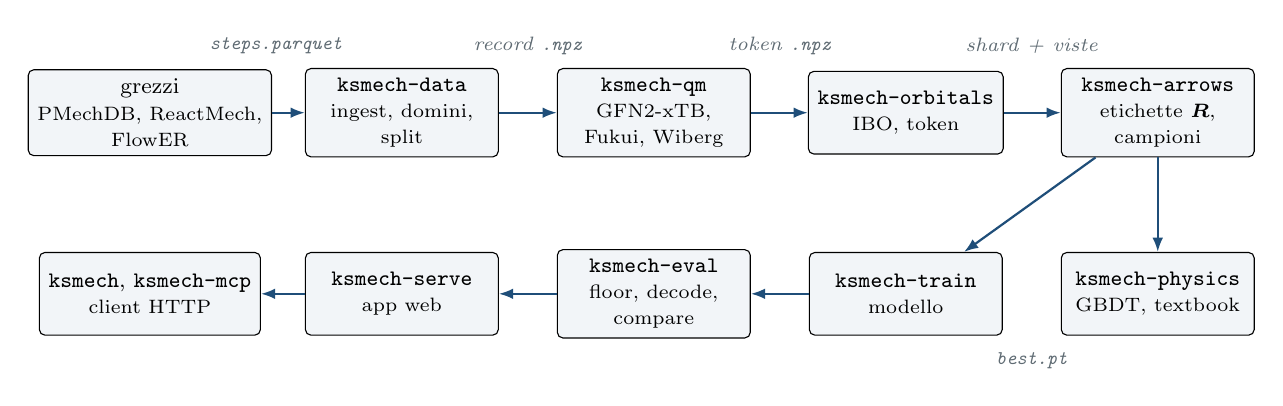
\begin{tikzpicture}[
  box/.style={draw, rounded corners=2pt, fill=ksfondo, font=\footnotesize, align=center,
              minimum width=2.45cm, minimum height=1.05cm},
  art/.style={font=\scriptsize\itshape, text=ksgrigio, align=center},
  arr/.style={-{Latex[length=1.8mm]}, thick, ksblu}]
\node[box] (raw) at (0,0) {grezzi\\\scriptsize PMechDB, ReactMech,\\\scriptsize FlowER};
\node[box] (data) at (3.2,0) {\code{ksmech-data}\\\scriptsize ingest, domini,\\\scriptsize split};
\node[box] (qm) at (6.4,0) {\code{ksmech-qm}\\\scriptsize GFN2-xTB,\\\scriptsize Fukui, Wiberg};
\node[box] (orb) at (9.6,0) {\code{ksmech-orbitals}\\\scriptsize IBO, token};
\node[box] (arr) at (12.8,0) {\code{ksmech-arrows}\\\scriptsize etichette $\vb{R}$,\\\scriptsize campioni};
\node[box] (phys) at (12.8,-2.3) {\code{ksmech-physics}\\\scriptsize GBDT, textbook};
\node[box] (train) at (9.6,-2.3) {\code{ksmech-train}\\\scriptsize modello};
\node[box] (eval) at (6.4,-2.3) {\code{ksmech-eval}\\\scriptsize floor, decode,\\\scriptsize compare};
\node[box] (serve) at (3.2,-2.3) {\code{ksmech-serve}\\\scriptsize app web};
\node[box] (cli) at (0,-2.3) {\code{ksmech}, \code{ksmech-mcp}\\\scriptsize client HTTP};
\draw[arr] (raw) -- (data); \draw[arr] (data) -- (qm); \draw[arr] (qm) -- (orb); \draw[arr] (orb) -- (arr);
\draw[arr] (arr) -- (phys); \draw[arr] (arr) -- (train); \draw[arr] (train) -- (eval);
\draw[arr] (eval) -- (serve); \draw[arr] (serve) -- (cli);
\node[art] at (1.6,0.85) {\code{steps.parquet}};
\node[art] at (4.8,0.85) {record \code{.npz}};
\node[art] at (8.0,0.85) {token \code{.npz}};
\node[art] at (11.2,0.85) {shard + viste};
\node[art] at (11.2,-3.15) {\code{best.pt}};
\end{tikzpicture}
\caption{La pipeline: ogni comando legge gli artefatti del precedente, verificandone la provenienza.}
\label{fig:pipeline}
\end{figure}

\section{Mappa dei pacchetti}
\begin{longtable}{@{}lrrp{10.2cm}@{}}
\caption{Sotto-pacchetti del motore (\code{src/ksmech}), escluso \code{serve}. Righe di codice Python.}
\label{tab:pacchetti}\\
\toprule
Pacchetto & File & Righe & Contenuto\\
\midrule
\endfirsthead
\toprule Pacchetto & File & Righe & Contenuto\\ \midrule
\endhead
\code{data} & 26 & 7\,625 & Loader delle sorgenti (\code{pmechdb}, \code{reactmech}, \code{rmechdb},
  \code{mech_uspto}, \code{qmugs}), validazione e ingest, leggi di dominio (\code{domain.py}, 955 righe:
  13 codici, 16 classi, \code{DomainPolicy}), ridisegni di spin (\code{pairing.py}), spin
  (\code{spin.py}, \code{spin_table.py}, \code{spin_theory.py}), risonanza e chiavi d'identità,
  split, audit di leakage, statistiche, indagine open-shell, provenienza; catene di pathway ReactMech
  (\code{pathways.py}) e benchmark umano (\code{human_benchmark.py}, \code{benchmark_checks.py}).\\
\code{qm} & 25 & 6\,191 & \code{QMConfig} e calcolatore GFN2, ottimizzatori (L-BFGS-B, ANC/RFO),
  embedding, batch con manifest e tombstone, record e cache, tag di spin, Fukui, indici di Wiberg,
  $V^{\mathrm{bur}}$, layout AO, preload OpenBLAS, single point QMugs, indice SQLite, rilevatore del
  gruppo puntuale (704 righe); Hessiane, termochimica quasi-RRHO, sidecar e batch termici,
  ri-ottimizzazione lungo i modi immaginari, liste di specie.\\
\code{orbitals} & 10 & 3\,262 & Localizzazione IBO/PM, descrittori, classificatore diagnostico,
  pesi di frontiera, token (\code{tokens.py}, 1\,068 righe: \code{CandidateConfig}, esclusioni,
  lacune), build del dataset, chiralità, gruppi funzionali.\\
\code{arrows} & 17 & 5\,581 & Frecce come modifica BE, allineamento diagnostico, \code{ReactionMatrix}
  ed etichette (\code{delta_be.py}), disegni di risonanza, chiusura per simmetria, struttura di Lewis,
  indice globale dei token, campioni (\code{steps.py}, 1\,106 righe), store a shard, collazione dei
  batch, round trip, H mobili di ReactMech, campioni all'indietro (\code{backward.py}).\\
\code{physics} & 10 & 2\,166 & Parametri (\code{K}, \code{BETA_INTER}), $G$ e $g_2$, accoppiamento WH,
  feature di coppia geometry-free, flag di coppia, statistiche, ranker LightGBM, casi da manuale.\\
\code{model} & 10 & 1\,967 & \code{ModelConfig} e preset, input non appresi, encoder denso/flex/sparse,
  decodificatore, loss, beam decoder, $\log P$ di una $\vb R$ data (\code{matrix_logp}).\\
\code{train} & 4 & 938 & \code{TrainConfig}, ciclo di training, batching a budget di celle, CLI.\\
\code{eval} & 13 & 2\,843 & Floor, decodifica, confronto appaiato, importanza per permutazione, coorti,
  pinning, traccia degli embedding come pagina HTML, esiti fratelli (\code{siblings.py}), riordinamento
  per andata e ritorno (\code{roundtrip.py}).\\
\code{network} & 24 & 4\,887 & Rete di reazione (capitolo~\ref{ch:rete}): chiavi di pool, grafo implicito
  e ricerca $k$-best, bersagli, espansore sul modello, catena di Markov, stop termodinamico, TPT,
  serbatoi, energie libere, grafo delle specie e iper-cammini, flusso atomico, retrosintesi, benchmark.\\
\code{client} & 8 & 1\,831 & Client HTTP \code{KsmechClient} e CLI \code{ksmech}.\\
\code{mcp} & 9 & 768 & Server MCP (FastMCP) sopra il client.\\
\code{processes.py} & 1 & 49 & Pool \emph{spawned} con un thread BLAS per processo.\\
\midrule
Totale motore & & 38\,192 & (l'app web \code{serve}: 113 moduli, 26\,101 righe; capitolo~\ref{ch:serve})\\
\bottomrule
\end{longtable}

\section{Comandi}
\begin{table}[H]
\centering
\caption{Punti d'ingresso (\code{[project.scripts]} di \code{pyproject.toml}).}
\label{tab:cli}
\small
\begin{tabular}{@{}lp{11.3cm}@{}}
\toprule
Comando & Sottocomandi principali\\
\midrule
\code{ksmech-data} & \code{ingest}, \code{stats}, \code{open-shell-survey}, \code{freeze-sample},
  \code{leakage-audit}, \code{provenance}, \code{pathways}, \code{human-benchmark}\\
\code{ksmech-qm} & \code{run} (anche \code{--species-from}, \code{--solvent}), \code{thermo}, \code{qmugs},
  \code{bond-index}, \code{index refresh|stats}\\
\code{ksmech-orbitals} & \code{build}, \code{show}, \code{fg-vocab}\\
\code{ksmech-arrows} & \code{roundtrip}, \code{align}, \code{samples}, \code{edit-labels}
  (entrambi con \code{--direction backward}), \code{coverage}, \code{freeze-splits}\\
\code{ksmech-physics} & \code{gbdt}, \code{textbook} (anche \code{--radical})\\
\code{ksmech-train} & \code{fit}\\
\code{ksmech-eval} & \code{floor}, \code{decode}, \code{compare} (\code{--metric own|any}),
  \code{importance}, \code{pin}, \code{cohort}, \code{embedding}, \code{roundtrip}\\
\code{ksmech-network} & \code{search}, \code{evaluate}, \code{predict}, \code{species}, \code{retro},
  \code{retro-eval}\\
\code{ksmech-serve} & server web e amministrazione (utenti, OCR, re-key, export)\\
\code{ksmech} / \code{ksmech-mcp} & client HTTP / server MCP\\
\bottomrule
\end{tabular}
\end{table}

\section{Dipendenze e ambienti}
Dipendenze del motore: \code{rdkit}, \code{numpy}, \code{scipy}, \code{pandas}, \code{pyarrow},
\code{tblite}, \code{morfeus-ml}, \code{tqdm}, \code{rich}, \code{lightgbm>=4.7.0} (aggiunto su
richiesta esplicita dell'utente quando il GBDT in numpy fu ucciso per memoria; la regola
\enquote{preferire numpy} è stata poi allentata dall'utente il 29 ottobre). \code{hydra-core} è
dichiarato ma inutilizzato: ogni configurazione è una dataclass congelata esposta via argparse.
Gruppi: \code{dev} (pytest, ruff, pre-commit, pytest-xdist), \code{serve} (FastAPI, uvicorn, SQLModel,
pydantic\dots), \code{client}, \code{mcp}, \code{rocm} (default: torch 2.14.1+rocm7.2 con triton-rocm
3.8.0) e \code{cuda} (torch 2.14.1 cu130), in conflitto tra loro. Il lock copre solo linux x86\_64.

\paragraph{Hardware.} Sviluppo e piccoli training su una AMD Radeon RX 6600 XT (8\,GB, gfx1032) con
ROCm 7.2: gfx1032 non ha kernel rocBLAS propri e serve \code{HSA_OVERRIDE_GFX_VERSION=10.3.0} (i kernel
gfx1030); senza, \code{torch.cuda.is_available()} è vero ma il primo kernel va in segmentation fault
(exit 139), quindi \code{ksmech-train} imposta l'override da sé quando rileva un target RDNA2 senza
kernel. Prodotti di matrici: 5{,}6 TFLOPS in float32, 8{,}0 in float16. I training di confronto girano
su pod NVIDIA noleggiati (RunPod, vast.ai): RTX 3090 Ti, RTX 5080, RTX 5090, 2$\times$RTX 3090. CPU
locale Ryzen 7 2700X (16 thread), 16\,GB di RAM dopo la rimozione di un modulo difettoso; regola: al
più 15 processi pesanti.

\section{Regole d'ingegneria}
\begin{itemize}
\item Mai inventare una colonna di dataset: aprire il file reale e documentarne lo schema in
  \code{docs/data_schema.md}.
\item Ogni funzione di featurizzazione ha un test sulle 10 molecole fisse (etano, etanolo, acetone,
  acetaldeide, acetato di metile, clorometano, metilammina, acetonitrile, benzene, acroleina) e, se una
  fase open-shell la cambia, sulla lista \code{OPEN_SHELL} (radicali, superossido, anione radicale del
  benzene, O$_2$ tripletto, Br$^\bullet$, $^\bullet$OH, NO, Cl[C]Cl, [C]=O, [N]=[N], ozono, CuCl$_2$,
  FeBr$_4^-$).
\item Nessun fallimento silenzioso; cache QM su disco; \code{pytest} prima di dichiarare finito un
  lavoro; ogni scelta non ovvia in \code{docs/decisions.md} con la data; funzioni sotto le 60 righe.
\item Ruff (lunghezza di riga 100, regole \code{E,F,I,UP,B,SIM,NPY}); hook di pre-commit: ruff, poi la
  suite non-realdata in 14 processi (pytest-xdist), poi i test su dati reali uno alla volta, ciascuno
  in 14 processi \emph{spawned}. Da 37 minuti su un core a pochi minuti: la regola del filtro dei
  candidati in forma chiusa ha portato il test di allineamento da 1\,441\,s a 11{,}7\,s.
\end{itemize}

\section{Test}
165 file \code{tests/test_*.py} (48 dell'app web), circa 1\,770 funzioni di test e 34\,300 righe;
l'ultima esecuzione (11 novembre, \code{f57a41f}) ha dato 2\,877 test di unità superati in 6 minuti e 23
secondi con 14 processi (12 saltati, 2 \emph{xfail} documentati); i test su dati reali erano 67 all'ultimo
commit verificato dall'hook. Marcatori: \code{realdata} (file grezzi reali, saltati se assenti; 22 file),
\code{slow} (ottimizzazioni GFN2), \code{diagnostic} (etichette del classificatore), \code{serve}
(app web con chimica sintetica o stub, mai xTB), \code{e2e} (Playwright, solo con \code{KSMECH_E2E=1}).
Test notevoli: invarianza per rotazione delle feature di coppia; nessun tensore di input del modello
contiene un tipo orbitale; la configurazione \code{pair_cells='valid'} riproduce bit per bit un batch
v17 (\code{test_legacy_reproduction.py}); stabilità degli split congelati; confine motore/app web
(\code{test_engine_boundary.py}: il motore non importa mai \code{ksmech.serve}).

\scoperta{l'hook di commit e le variabili di git}{Due \code{git commit --only} fallivano con
\enquote{files were modified by this hook}: git esporta un indice temporaneo come
\code{GIT_INDEX_FILE}, e un test che eseguiva \code{git init/add/commit} in un repository di prova
scriveva in quell'indice (una copia dell'indice reale passò da 154 file a 1). Da allora
\code{provenance.git_env()} toglie tutte le variabili \code{GIT_*} per i comandi git interni e per i
test.}
% =====================================================================
\chapter{Dati: sorgenti, ingest e leggi di dominio (\texttt{ksmech.data})}
\label{ch:dati}
% =====================================================================

\section{Le sorgenti}
\begin{longtable}{@{}p{2.6cm}p{12.6cm}@{}}
\caption{Sorgenti di dati e loro ruolo.}\label{tab:sorgenti}\\
\toprule
Sorgente & Ruolo e caratteristiche\\
\midrule
\endfirsthead
\toprule Sorgente & Ruolo e caratteristiche\\ \midrule
\endhead
PMechDB & Passi polari curati a mano, con frecce come indici di mappe atomiche. Set di sviluppo.
  Si ingeriscono i 13\,104 record \code{mc_only} della release PMechRP (\code{fold0/raw/*.txt}; ogni
  fold e lo split per scaffold sono permutazioni dello stesso insieme); gli split \enquote{mixed}
  aggiungono 10\,000 trasferimenti di protone generati combinatorialmente e sono esclusi. Nessuna
  classe, pathway, ordine dei passi o condizione: ogni passo è isolato. \code{step_id} =
  \code{"pmechdb-"} + i primi 16 caratteri dello SHA-1 del testo grezzo.\\
ReactMech & 67 classi di reazione, passi mappati \emph{senza frecce}; l'etichetta è la differenza
  dei due lati (capitolo~\ref{ch:etichette}). Usato per split fuori distribuzione; pilota da 10\,000
  passi (licenza CC BY 4.0).\\
RMechDB (\code{rmechdb}) & Passi radicalici (a un elettrone): per ora le righe RS/RC di FlowER,
  in futuro il CSV ufficiale. 4\,535 passi dopo la deduplicazione; split \code{rc_molecule} (RC per
  molecola, RS in training). Licenza CC-BY-NC-ND: artefatti solo locali, nel dataset privato e sui pod,
  mai pubblici.\\
FlowER & Circa 2{,}14 milioni di righe con suffisso numerico (train+val+test), generate da template
  su USPTO-Full. Destinato allo scale-up; le sue righe RS/RC sono ingerite come rmechdb, PM e PC mai.\\
mech-USPTO-31K & Benchmark tenuto da parte, mai usato in training. Una riga per reazione con una
  lista piatta di frecce, senza confini tra passi: \code{load} solleva \code{NotImplementedError},
  perché una conversione parziale produrrebbe falsi passi elementari.\\
QMugs & Circa 665\,000 molecole drug-like; per il pre-addestramento dell'encoder sono previsti
  single point GFN2-xTB alle geometrie di QMugs (batch di 100\,000 avviato, solo locale).\\
\bottomrule
\end{longtable}

\section{Canonicalizzazione e schema}
\begin{itemize}
\item Le molecole sono lette con \code{removeHs=False} (gli H mappati sono estremi di frecce) e
  sanitizzate con \code{SANITIZE_ALL ^ SANITIZE_SETAROMATICITY}: niente percezione dell'aromaticità,
  perché PMechDB è scritto in forma di Kekulé e le frecce nominano legami singoli e doppi specifici.
  Verificato: 0 delle 26\,182 stringhe canoniche di PMechDB porta atomi aromatici.
\item La stringa canonica è \code{MolToSmiles(..., kekuleSmiles=True)} sull'intero lato
  multi-frammento, mappe incluse (due forme di Kekulé danno stringhe diverse, di proposito);
  l'identità di molecola per statistiche e scaffold usa una chiave separata senza mappe.
\item Una freccia è salvata \emph{come disegnata} (coda: doppietto, legame o radicale; testa: atomo o
  legame); \code{Arrow.destination()} ne deriva la destinazione. La rappresentazione è senza perdite.
\item Ordine di validazione: parsing $\to$ bilancio degli atomi pesanti (\code{UNBALANCED}) $\to$
  bilancio di H $\to$ bilancio di carica $\to$ unicità e biiezione delle mappe $\to$ atomi delle frecce
  mappati $\to$ legami sorgente presenti (\code{BOND_NOT_FOUND}) $\to$ \textbf{replay delle frecce}: le
  frecce applicate come un'unica modifica della matrice BE devono riprodurre i prodotti modulo
  risonanza (\code{ARROWS_MISMATCH}; decisione dell'utente del 20 ottobre).
\item Re-ingest di PMechDB: 13\,104 record $\to$ 13\,090 accettati, 14 rifiutati (12
  \code{SANITIZE_FAILED}: complessi \emph{ate} ipervalenti come \code{Br[Br-]Br}; 1
  \code{MAP_NOT_BIJECTIVE}; 1 \code{ARROWS_MISMATCH}, un Na dativo che sparisce senza freccia). Round
  trip delle frecce del dataset: 100\% dei passi di training.
\end{itemize}

\section{Il dominio: esclusioni e riparazioni contate}
\label{sec:dominio}
Ogni motivo per cui un passo non è un campione di training è un codice contato in \code{stats.json};
la frazione coperta è riportata accanto a ogni accuratezza. La storia di queste regole è istruttiva.

\paragraph{Prima versione (21--24 ottobre).} Un frammento con numero di elettroni dispari senza
elettroni radicalici in RDKit non è calcolabile a guscio chiuso. Un'indagine su tutti i 14\,382
frammenti unici di PMechDB ne trovò 100 (non solo i 20 \code{SPIN_PARITY} già incontrati dal batch),
tutti tranne uno con un metallo. Regole: \code{METAL_PLACEHOLDER} (metallo non alcalino con al più un
vicino: catalizzatori di Lewis disegnati senza leganti, \code{C=[O+][Ti]}), \code{CHARGE_REPAIRED}
(R1: si toglie un $-1$ da un atomo del gruppo 14 tetravalente; R2: legame onio$\to$accettore
d$^0$/d$^{10}$ letto come dativo), \code{OPEN_SHELL_METAL} (soprattutto addotti di Cu(II) e Fe(III)),
\code{CHARGE_UNREPAIRED}. Il 24 ottobre si aggiunse \code{RADICAL_DRAWN}: 51 passi con atomi radicalici
in RDKit, quasi tutti errori di disegno (metili scritti \code{[C:20]} senza H, letti come quartetti).

\paragraph{Leggi unificate (P0a, 29 ottobre).} Il principio \enquote{nessuna regola arbitraria} ha
sostituito le regole condizionate da elemento e parità con una legge per fenomeno:
\begin{description}[style=nextline]
\item[Legge dativa (\code{D dative onium->M})] un onio (non metallo positivo diverso da C) legato a un
  metallo o a B è un donatore dativo; l'accettore è ricaricato del massimo $j$ che lascia pari il
  numero di elettroni del frammento, la carica netta del lato $\ge0$ e i totali dei due lati uguali;
  poi il passo è rivalidato. La forma letterale (\enquote{il metallo prende $-1$ per onio}) è stata
  scartata dopo la misura: avrebbe ricaricato a torto 101 passi PMechDB e 58 ReactMech. Un audit dello
  stato di ossidazione su 20 casi (\code{scripts/probes/dative_audit.py}) li ha trovati tutti corretti.
\item[Legge del segnaposto] un metallo fuori dal blocco $s$ con esattamente un vicino e carica $\le0$ è
  un catalizzatore disegnato senza leganti, a qualunque parità (\code{METAL_PLACEHOLDER}), tranne
  quando compensa un donatore onio (ML$_1$, \code{[Pd-][P+]R3}); ioni liberi e MX$^+$ sono specie
  definite.
\item[\code{METAL_SUSPECT}] un frammento pari con un metallo 3d lasciato d$^1$--d$^9$ dalla
  contabilità degli stati di ossidazione: un flag, mai un'esclusione.
\end{description}
Effetti misurati: su PMechDB la legge dativa cambia 0 passi, quella del segnaposto ne rimuove 24 e gli
8 passi con Sn passano da \code{RADICAL_DRAWN} a \code{METAL_PLACEHOLDER} (passi di training 12\,464
$\to$ 12\,442); sul pilota ReactMech 49 passi sono ricaricati (25 Ni, 24 Pd) e 205 passi esclusi tornano
nel dominio (109 Pd(0) L$_1$, 96 \code{OPEN_SHELL_METAL}).

\paragraph{Riparazioni di disegno (P1, 30 ottobre).} Applicate prima delle altre leggi, conservate
solo se il passo si rivalida e solo su atomi disegnati allo stesso modo nei due lati:
V1 (un C neutro con 3 elettroni radicalici e un vicino riceve 3 H; il C-2 dell'imidazolo di CDI
riconosciuto per topologia riceve un H), A1 (un atomo alcalino neutro nudo riceve $+1$), \code{BL_NAMED}
(l'unico azoto $\beta$-lattamico di PMechDB disegnato senza H, riparazione nominata di un singolo
passo). Su PMechDB: 9 metili, 4 K/Na nudi, 1 $\beta$-lattame; \code{RADICAL_DRAWN} 44 $\to$ 30. Su
ReactMech: 62 passi CDI.

\paragraph{Stato attuale di PMechDB} (\code{data/processed/pmechdb/stats.json}): 13\,090 passi, 482
passi di risonanza, \textbf{12\,512 passi di training}. Esclusioni: \code{RESONANCE_STEP} 482,
\code{METAL_PLACEHOLDER} 56, \code{MULTIPLICITY_AMBIGUOUS} 36, \code{RADICAL_DRAWN} 5,
\code{SPIN_NOT_CONSERVED} 2, \code{CHARGE_UNREPAIRED} 1; 15 riparazioni di carica conservate (V1 9,
A1 4, R1 1, BL 1). Classi di dominio ammesse: \code{CARBENE_SINGLET} 12, \code{OSM_CU2} 23,
\code{OSM_FE3} 19, \code{RADICAL_SPECTATOR} 11. Frecce per passo: 1 (2\,401), 2 (8\,570), 3 (1\,960), 4
(156), 5 (3). Frammenti reagenti 29\,404 (10\,683 unici, 2{,}25 per passo); atomi pesanti per passo:
mediana 16, media 20{,}5, massimo 220.

\section{Identità di risonanza}
\label{sec:risonanza}
Prodotti ed etichette sono confrontati modulo risonanza. La chiave d'identità ha avuto quattro
generazioni:
\begin{enumerate}
\item \textbf{chiave enumerata con mappe} (20 ottobre): lo SMILES canonico minimo sulle strutture di
  \code{ResonanceMolSupplier}, al più 1\,000; dipendeva dall'ordine degli atomi (il fenossido dava due
  chiavi) e veniva troncata nel 7\% dei lati;
\item \textbf{chiave enumerata senza mappe} con H congelati (22 ottobre), test per intersezione di
  insiemi invece che per uguaglianza dei minimi (RDKit enumera C=N--X da C$^+$--N$^-$--X ma non il
  contrario);
\item \textbf{chiave sigma} (25 ottobre, \enquote{opzione B} scelta dall'utente): lo SMILES canonico
  senza mappe dello scheletro $\sigma$ (ogni legame singolo, niente aromaticità né stereochimica),
  con il numero di H di ogni atomo congelato, cariche ed elettroni spaiati azzerati, seguito dalla
  carica totale. Due strutture di Lewis a guscio chiuso con la stessa chiave hanno gli stessi atomi,
  legami $\sigma$, H e carica totale, quindi lo stesso numero di elettroni: sono forme di risonanza.
  Non enumera nulla, quindi è esatta e mai troncata;
\item \textbf{chiave d'identità v2} (P6, 4 novembre): per un disegno senza elettroni spaiati è la chiave
  sigma (ogni chiave a guscio chiuso resta invariata); per un guscio aperto vi aggiunge il multiinsieme
  ordinato di (SMILES sigma del frammento, carica, numero di spaiati). Separa un radicale dal suo ione e
  D$^\bullet$+A da D$^+$+A$^{\bullet-}$, mentre \code{[C]=O} e \texttt{[C-]\#[O+]} restano una specie.
\end{enumerate}

\scoperta{RDKit non è un test di appartenenza alla risonanza}{La chiave enumerata concordava tra le
forme di risonanza di un prodotto solo nel 59\% dei prodotti campionati di PMechDB (l'InChI con H fissi
nel 58\%); la chiave sigma nel 100\%. Inoltre, dal reagente disegnato RDKit raggiunge il prodotto
disegnato solo in 147 delle 471 coppie di risonanza di PMechDB, perché non enumera a partire da centri
con ottetto incompleto; e \code{ResonanceMolSupplier} restituisce \enquote{non forme}: rideriva gli H
degli atomi non tra parentesi (un O del nitro diventa \code{[OH2+]}) e restituisce strutture
radicaliche (l'azide come N=N--N con due radicali). Le forme usate per le classi di etichette e per
l'augmentation sono quindi quelle di RDKit con H congelati, filtrate per stesso numero di H per atomo,
carica totale ed elettroni spaiati.}

\paragraph{Passi di risonanza e coppie.} Un passo i cui due lati hanno la stessa chiave d'identità
con le mappe conservate e un flusso elettronico bilanciato non cambia legami $\sigma$, H, carica o spin
di alcun atomo: è un'interconversione di risonanza, esce dal bersaglio di training ed è conservato come
\emph{coppia di risonanza} (\code{resonance_pairs.parquet}; 482 dei 13\,090 passi PMechDB accettati,
548 dei 10\,000 del pilota ReactMech). Lati identici sono \code{NULL_STEP}, stessa chiave senza flusso
bilanciato \code{NONCONJUGATED_SHIFT}: entrambi contati, nessuno è una coppia di risonanza. Gli
\textbf{scambi degeneri} (stesse molecole, atomi che cambiano partner: scambio tiolo--disolfuro,
scambio di protone tiolato/tiolo, shift cationico degenere in una gabbia simmetrica) sono passi reali e
restano (3 su PMechDB; decisione dell'utente del 25 ottobre: \enquote{un meccanismo segue gli atomi}).

\section{Split, snapshot congelati e coorti}
\label{sec:split}
\paragraph{Split per molecola (default).} Due passi che condividono una molecola non banale (SMILES
canonico senza mappe con stereochimica, più di 3 atomi pesanti; acqua, H$_3$O$^+$, OH$^-$, alogenuri,
ioni metallici, MeOH e NH$_3$ ignorati), \textbf{nei reagenti o nei prodotti}, finiscono nella stessa
parte. Contare solo i reagenti lasciava attraversare le parti al 32\% dei collegamenti tra passi
(X$\to$Y e Y$\to$Z non condividono reagenti), quanto uno split casuale; con i prodotti, 0. Il costo:
i reagenti comuni (HSO$_4^-$, H$_2$SO$_4$, AcO$^-$, AcOH, TsO$^-$, Et$_3$NH$^+$, TFA$^-$, piridina)
legano il 78\% dei passi in un unico gruppo che va in training; validazione e test vengono dal 22\%
restante e sono quindi fuori distribuzione per costruzione. Lo split per passo è stato rinominato
\code{random_leaky} (con lo stesso seed, 457 passi di test avevano il reagente più grande in training)
e si costruisce solo se nominato; il vecchio nome \code{random} solleva un errore.

\paragraph{Altri split.} \code{scaffold} (scaffold del frammento reagente più grande; lo scaffold
aciclico è un gruppo del 37{,}5\% che va in training), \code{loco} (leave-one-class-out, per sorgenti
con classi: su ReactMech le classi acid-halide, anhydride, carbamic-halide, haloformate, sul-halide),
\code{loco_all} (la classe tenuta fuori come test, i passi senza classe in train e val),
\code{rc_molecule} e \code{flower_given} per rmechdb.

\paragraph{Snapshot congelati (U1).} Gli split sono \emph{append-only}: uno snapshot di ogni split,
con uno schema proprio (\code{FROZEN_SPLIT_SCHEMA}) che nessuna versione dei campioni invalida, tiene
ogni passo esistente nella sua parte quando si aggiungono passi o si ricostruiscono i dati. Un gruppo
che contiene passi congelati mantiene la loro parte, un gruppo nuovo è piazzato con un hash della sua
chiave, e un passo nuovo che unisce gruppi congelati in due parti diverse è lasciato fuori e contato
(\code{SPLIT_CONFLICT}). Uno snapshot si sostituisce solo a mano (come in P4, quando i passi con Cu
hanno unito gruppi e lo snapshot per molecola di PMechDB è stato esteso).

\paragraph{Coorti.} Una coorte è un insieme fissato di id di passi; ogni numero è riportato per
coorte. \code{closed_base} (fissata il 29 ottobre, codice \code{d1b869b}) è l'insieme dei campioni
PMechDB dello split per molecola dopo P0a: train 9\,979, val 1\,238, test 1\,182 (12\,399), con digest
per colonna di ogni campione (64 colonne, ciascuna un SHA-256 troncato a 64 bit, 18{,}7\,MB); i
cambiamenti successivi sono verificati confrontando questi digest per contenuto. I dati aggiunti
formano coorti proprie e non sono mai mescolati in un numero di riferimento: \code{added} (13 passi
riparati in P1), \code{open_shell} (9), \code{carbene_singlet} (10), \code{open_shell_metal} (38),
\code{p5_returns}, e le coorti di leakage di rmechdb (\code{leak_guard_joint},
\code{rc_heldout_overlap}, \code{rc_heldout_shared}, \code{closed_base_rmechdb_overlap}).

\section{Provenienza degli artefatti}
\label{sec:provenance}
Ogni artefatto ha un'intestazione \code{Provenance} (\code{kind}, \code{schema_version},
\code{code_git_hash}, \code{code_dirty} e \code{code_diff_sha256}, \code{spec_sha256} della specifica,
\code{inputs} con lo SHA-256 di ogni input, \code{config}, \code{built_at}, \code{content_sha256}); nei
\code{.npz} è il membro \code{__provenance__}, nei JSON la chiave \code{provenance}. Le catene: record
QM (input: SMILES canonico; config: metodo, solvatazione, conformero) $\to$ file di token (input: il
record; config: \code{DescriptorConfig} e parametri di localizzazione) $\to$ shard dei campioni (parquet,
token) $\to$ indice $\to$ vista per split $\to$ checkpoint e report. I loader confrontano schema, config
e input e rifiutano un artefatto obsoleto (\code{STALE_ARTIFACT}); training e valutazione rifiutano
build da un albero sporco (\code{require_clean}; l'hash copre \code{git diff HEAD} più i file non
tracciati sotto \code{src/}). Hash del codice, della specifica e data sono solo tracciamento, così un
commit da solo non invalida le cache. \code{ksmech-data provenance <artefatto>} stampa la catena e dice
se è obsoleta.

\scoperta{modificare file tracciati durante una build}{Poiché il flag di albero sporco copre
\code{git diff HEAD}, modificare un file tracciato (anche la specifica o un test) mentre una build gira
rende i suoi output rifiutati. È successo una volta durante P4 (modifiche ai test, annullate in pochi
minuti, nessun record risultato sporco); da allora la regola è non toccare file tracciati durante una
build.}

\section{Dataset privato}
I dati derivati (store dei campioni, 20\,885 file di token e altrettanti sidecar di Wiberg impacchettati
in 17 archivi tar da circa 500\,MB) sono su un dataset Hugging Face privato (\code{rhoMech-data}): la
versione v18 occupava 210 file e 9{,}63\,GB (upload 73 minuti, download 20); la revisione attuale
contiene lo store 19 delle tre sorgenti più la sovrapposizione \code{release_a/} (store 18 per P4).
Privato per i termini di PMechDB (via PMechRP, non stabiliti) e la licenza NC-ND di RMechDB; un pod
riceve un token di sola lettura cancellato dopo il download.
% =====================================================================
\chapter{Il piano open-shell (fasi P0--P9)}
\label{ch:openshell}
% =====================================================================
Il piano per portare i gusci aperti in \ksm\ (\code{docs/open_shell_plan.md}) è stato concordato il
28 ottobre con 23 decisioni (U1--U23). La sua filosofia: i gusci aperti non erano mai stati rifiutati
da una decisione unica, ma rimandati regola per regola (\code{RADICAL_DRAWN},
\code{OPEN_SHELL_METAL}, \code{SPIN_PARITY}, \code{METAL_PLACEHOLDER}, la maschera
\code{fermi_smeared}). Nessuno dei 290 passi esclusi di PMechDB e del pilota ReactMech era un passo
radicalico: quasi tutti erano errori di disegno. Il piano lavora \enquote{dall'esterno verso
l'interno}: prima generalità e riferimento, poi i gusci aperti nei passi polari (Release A), poi la
contabilità elettronica e i passi radicalici (Release B), infine il modello.

\begin{table}[H]
\centering
\caption{Fasi del piano open-shell.}
\label{tab:fasi}
\small
\begin{tabular}{@{}lp{2.1cm}p{10.6cm}@{}}
\toprule
Fase & Data & Contenuto\\
\midrule
P0 & 28 ott & Infrastruttura: snapshot di split congelati, coorti, versioni di floor e decoder.\\
P0a & 29 ott & Generalità: tutte le celle di coppia con flag, extra orbitali, finestra di frontiera
  esatta, etichette ReactMech dal Kekulé più vicino, caps per sorgente, leggi di dominio unificate
  (\code{SAMPLE_VERSION} 18, token schema 10, spec v9.1).\\
P0b & 29--30 ott & Coorte \code{closed_base}, confronto appaiato, preset; GENERAL contro LEGACY su pod.\\
P1 & 30 ott & Riparazioni di disegno V1, A1, \code{BL_NAMED}.\\
P2 & 31 ott & Ogni molteplicità derivata due volte (scansione spGFN2 e teoria) e combinata:
  \code{spin_theory_v1}, \code{spin_table_v1}.\\
P2b & 31 ott & Occupazioni di riferimento a plateau, frontiera radicalica, \code{atom_fukui}
  (spec v9.2).\\
P3 & 31 ott & Gusci aperti nei passi polari di PMechDB, ammessi da tre leggi contate.\\
v2 & 1 nov & \code{spin_table_v2}: dialocarbeni e difenilvinilidene decisi.\\
P4 & 3 nov & Spin da \code{data.spin.assign}, record QM etichettati, tabella dei metalli (Cu(II),
  Fe(III)), coorte dei metalli.\\
P5 & 4 nov & Ritorni del pilota ReactMech (riparazioni dative), audit dativo, ri-valutazioni per
  fetta. Fine della \textbf{Release A}.\\
P6 & 4 nov & Contabilità elettronica: $u$ dal disegno, legge del flusso, chiave d'identità v2,
  codici \code{SET_STEP}/\code{DISSOCIATIVE_ET_STEP}, \code{SAMPLE_VERSION} 19.\\
P7 & 5 nov & SOMO donatori e lacune, popolazione SOMO, $G$ pesato per occupazione, $g_2$, canali
  own-pair e di ricombinazione, floor \code{own_break}.\\
P8 & 5--6 nov & RMechDB via FlowER, un'unica legge di spin e dominio, build della \textbf{Release B};
  spec v10 approvata.\\
P9 & 6--9 nov & Testa atomica a cinque classi, schermo di decodifica, preset \code{open_shell};
  training (passi 8 e 9).\\
\bottomrule
\end{tabular}
\end{table}

\section{La regola di tolleranza U20}
Ogni anello della catena di confronti (Release A contro P0b GENERAL; \code{pm_control} contro Release
A; \code{joint} contro \code{pm_control}) usa la stessa regola, unilaterale sul top-1 full-R di
\code{closed_base} val: il braccio A fallisce quando la sua media è più bassa di più di
$\max(2\times$ deviazione standard combinata delle 6 run dell'anello$,\ 1$ punto$)$. Accanto si riporta
il test esatto di McNemar unilaterale, $p=P(X\ge n_{ab})$ con $X\sim\mathrm{Bin}(n_{ab}+n_{ba},\tfrac12)$,
in aritmetica intera, sui \emph{hit} a maggioranza dei tre seed e sulle 9 coppie di seed
(\code{eval.paired}, \code{ksmech-eval compare}). Il confronto rifiuta bracci decodificati su campioni,
parti, coorti, beam, caps o versioni del decoder diversi. Regola di default di P9 passo 9: una regola
(maschera o filtro) è attiva di default solo se il test appaiato la mostra migliore ($p<0{,}05$) senza
cali su \code{closed_base}; un input fisicamente motivato resta se è migliore o non inferiore entro la
tolleranza.

\section{Spin: tabelle e leggi}
\label{sec:spin}
\paragraph{Due derivazioni indipendenti (P2).} Su richiesta dell'utente (\enquote{fai le due cose in
parallelo: il calcolo spGFN2 e le regole chimiche come la teoria del campo dei leganti, la teoria delle
rappresentazioni\dots}) ogni molteplicità è derivata due volte:
\begin{description}[style=nextline]
\item[(A) calcolo] spGFN2 ottimizzato in ALPB acqua a ogni molteplicità ammessa (Fe(III) a $S=5/2,3/2,1/2$,
  Cu(II) come controllo, specie di FlowER con $u\ge3$), conclusivo quando lo stato più basso sta sotto
  ogni altro di più della barra d'errore del metodo: organici 7\,kcal/mol $=0{,}304$\,eV (spGFN2 su
  AC12), metalli di transizione 17{,}9\,kcal/mol $=0{,}776$\,eV (MAD di spGFN2 sul sottoinsieme 3d di
  TM90S, Neugebauer et al.\ 2023);
\item[(B) teoria] \code{spin_theory_v1}: conteggio d$^n$, campo dei leganti (O$_h$: d$^{1-3}$, d$^8$,
  d$^9$, d$^{10}$ esito unico; d$^{4-7}$ dipendente dal campo; T$_d$ alto spin), gruppo puntuale e
  irrep di frontiera, regola di Hund, Gleiter--Hoffmann per i carbeni; nessuna regola nomina una specie;
\item[(C) combinazione] (scelta dall'utente) A e B concordano $\to$ assegna; B indeterminata $\to$ A
  decide entro la sua barra; ogni disaccordo $\to$ \code{MULTIPLICITY_AMBIGUOUS}.
\end{description}
Su 156 specie (64 organiche, 61 Cu/Fe, 31 \code{METAL_SUSPECT}): concordi 59, B indeterminata e A
conclusiva 37, A inconclusiva 15, disaccordo 5, A fallita 40. Fe(III) ad alto spin confermato per 13 su
20 specie di Fe e mai contraddetto; Cu(II) $u=1$ per 36 su 41.

\scoperta{il punto di sella lineare dei carbeni}{ETKDG disegna Cl[C]Cl e Br[C]Br esattamente lineari
(180{,}0°). Da quel punto di sella il tripletto sembrava più basso (0{,}69/0{,}64\,eV); da una partenza
spostata di 0{,}02\,Å CCl$_2$ si piega a 112{,}9° (singoletto) e il singoletto risulta più basso di
1{,}01\,eV (CBr$_2$: 0{,}76\,eV). Da qui due leggi: ogni stato è ottimizzato da due partenze
(l'embedding e un \enquote{calcio} di 0{,}02\,Å, seed 0) e si tiene il più basso convergente; e
\code{BOND_FORMED}: una partenza fallisce se due atomi non metallici a distanza di grafo $\ge2$ finiscono
entro $1{,}2\times$ la somma dei raggi covalenti (un epossido, un biradicale di Norrish II che si chiude
a ciclobutano, lo shift di Fritsch--Buttenberg--Wiechell del Ph$_2$C=C:).}

\paragraph{\code{spin_table_v2} (1 novembre).} L'utente ha scelto quattro cambiamenti alla tabella
invece di un arbitro DFT (PySCF non installato): B riottimizza dalla partenza spostata quando questa
finisce più bassa di $10^{-5}$\,Ha; regola 4a, un vinilidene R$_2$C=C: è singoletto (Stang 1978); regola
4b, un carbene con due vicini $\pi$-donatori con doppietto è singoletto (Bourissou 2000); in A, uno
stato di carbene che forma un legame da ogni partenza prende il single point verticale alla geometria
di produzione come limite superiore. Risultato: CCl$_2$, CBr$_2$, Ph$_2$C=C: $\to$ singoletto;
\code{COC(=O)[C]C(=O)OC} $\to$ tripletto; nessun verdetto su metalli o biradicali cambia.

\paragraph{Le leggi di dominio dei gusci aperti (P3).} Una specie disegnata con elettroni spaiati in un
passo polare è nel dominio quando valgono tre leggi, ognuna con il suo codice: (u) il suo numero di
spaiati (RDKit se $\le1$, altrimenti la tabella) si conserva nel passo (\code{SPIN_NOT_CONSERVED});
(R) ogni voce atomica di $\vb{R}$ è pari, cioè un passo polare non crea, distrugge o sposta un elettrone
spaiato (\code{NOT_ELEMENTARY}); (S) la sua SOMO è intera (\code{SOMO_NOT_INTEGRAL}). Un passo ammesso è
\code{RADICAL_SPECTATOR} o \code{RADICAL_REACTIVE}. PMechDB ammette per regola, le altre sorgenti
polari escludono. Ammessi 9 campioni (una riduzione di Birch, tre deprotonazioni di perossili, quattro
perossili $\to$ superossido, una protonazione del superossido) più 2 coppie di risonanza; un file di
curation elenca 5 passi che le leggi ammettono ma una lettura del disegno rifiuta. Il dodicesimo caso,
l'addotto Et$_3$B--O$_2$ (\code{5d007b38}), resta \code{SPIN_NOT_CONSERVED}: la tabella gli assegna
$u=0$; la decisione è lasciata all'utente.

\paragraph{Metalli (P4).} \code{data.spin.assign} restituisce conteggio, sorgente
(\code{rdkit}/\code{species}/\code{metal}) e motivo. Tabella dei metalli \code{metal_v1.json}: Cu(II)
$u=1$, Fe(III) ad alto spin $u=5$ senza donatori C o P, Cu(II) con donatore H o I incompatibile (il Cu(II)
li ossida); ogni riga vale per una specie solo dove la tabella delle specie la conferma (regola C).
\code{OPEN_SHELL_METAL} 78 si divide in \code{OSM_CU2} 23, \code{OSM_FE3} 19, \code{MULTIPLICITY_AMBIGUOUS}
36 (12 Cu, 24 Fe, di cui 14 Br$_2$--FeBr$_4^-$). 49 specie calcolate con etichetta di spin (48 riuscite;
l'addotto Et$_3$B--O$_2$ fallisce come \code{BOND_FORMED}). La legge (S) legge solo i frammenti disegnati
con elettroni radicalici (decisione dell'utente: un Cu(II) con smearing resta un campione marcato).

\paragraph{Contabilità elettronica (P6).} $u$ è il numero di atomi con $N_i$ dispari nel disegno
(\code{spin_of_drawing}); la tabella lo alza, mai lo abbassa: una riga di Hund (nella v2 solo [O] e
[O][O]) vale per ogni disegno con la sua chiave, così O=O, [O][O] e [O$^+$][O$^-$] sono un unico
tripletto; le altre righe valgono solo per il disegno scansionato. $N$ è letto da ogni disegno perché la
percezione dei radicali di RDKit separerebbe \code{[C]=O} da \texttt{[C-]\#[O+]} e conterebbe male
[Br$^+$], [OH$^+$] e il CH$_2$ di singoletto. Le forme di un radicale si ottengono con un
\emph{proxy anionico}: ogni centro radicalico prende un elettrone in più, si enumerano le forme
dell'anione, e in ogni forma ogni atomo negativo del gruppo coniugato restituisce l'elettrone e porta il
radicale (benzile e fenossile 4 forme, pentadienile 3, allile 2, TEMPO 1; NO$_3^\bullet$ un disegno per O).

\paragraph{Un'unica legge di spin (P8).} Un singoletto di tabella disegnato con $N$ dispari è ridisegnato
a guscio chiuso dove gli spostamenti di elettroni lungo i legami lo raggiungono
(\code{PAIRED_DRAWING}: N\#N, ozono, Criegee; ordinamento: ottetti completi, meno cariche, minore
$\sum q\chi$ di Pauling, così il Criegee è C=[O$^+$][O$^-$], meno legami cambiati; i metalli non sono
mai ridisegnati); un caso di Hund disegnato appaiato è ridisegnato spaiato (\code{HIGH_SPIN_DRAWING}:
O=O); una specie non metallica con $u\ge2$ che non è un caso di Hund, o un singoletto che nessun disegno
a guscio chiuso raggiunge, è \code{MULTI_RADICAL_SPECIES}, salvo esenzioni contate. Il censimento di
spin prima del QM rifiuta 37 specie rmechdb (\code{SPIN_CENSUS_REFUSED}). Una sorgente di passi a un
elettrone conserva $u$ solo dove $\vb{R}$ non sposta un singolo elettrone.

\section{RMechDB via FlowER (P8)}
FlowER ha 2\,174\,470 righe, 2\,140\,367 con suffisso numerico (righe train/test: RC 1\,383/136, RS
3\,223/346, PM 12\,322/294, PC 14\,746/1\,653; nessuna validazione). Il loader \code{data.rmechdb} toglie
i gas di bagno, applica i ridisegni di spin prima di calcolare l'id (reazione canonica senza mappe) e
tiene un passo per id, RC prima di RS: 5\,088 righe $\to$ 4\,535 passi (553 \code{DUPLICATE_STEP}, 165
righe con gas di bagno). QM a 14 worker: 4\,277 specie, 4\,227 record, 13 fallimenti, 37 rifiutate.
Etichette 4\,293/4\,333 (99{,}08\%; restano 11 reazioni radicaliche dell'ozono, che la legge del flusso
rifiuta con l'ozono disegnato O=[O$^+$][O$^-$], e l'omolisi del persolfato). Split \code{rc_molecule}:
RC 950/118/120 passi + 3\,096 RS in training; campioni 3\,916/111/113. \code{flower_given}:
3\,782/106/445. Campioni totali 4\,184 (\code{SOMO_NOT_INTEGRAL} 109).

\paragraph{Audit di leakage} (\code{ksmech-data leakage-audit}, specie per chiave v2): 36 passi di
training rmechdb condividono una specie con val/test di \code{closed_base} (\code{cohort_leak_guard_joint},
tolti dal training congiunto come \code{LEAK_GUARD}); 79 passi di training PMechDB condividono una specie
con val/test RC (una fetta, mai rimossi); 26 passi val/test RC con il training di PMechDB.

\section{Release B e merge}
Store \code{SAMPLE_VERSION} 19: PMechDB 12\,469 campioni, ReactMech 9\,256, rmechdb 4\,184; rispetto
alla v18 ReactMech è identico e PMechDB differisce solo nei 9 campioni \code{RADICAL_SPECTATOR}
(lacune). Migrazione in \code{main} via reflink (12\,122 file nuovi, 182 sostituiti; le copie v18 in
\code{data/processed/v18_reference/}), re-key dei 1\,388 stati di pool salvati dall'app web (69
cambiati), merge \code{87d8956} (P6 con P0--P5), \code{840e481} (P7), \code{5417210} (P8), poi il codice
P9 (\code{73fb691}); niente è stato pubblicato sul remoto. Il controllo di provenienza su 438\,802 file
ne ha trovati 432\,251 validi e 211 obsoleti (run e decodifiche vecchie).

\section{P9: il modello open-shell}
\begin{itemize}
\item Testa atomica $\{-2,-1,0,+1,+2\}$ (preset \code{open_shell}); $-1$ richiede $N\ge1$, $-2$ richiede
  $N\ge2$; nessuna maschera a livello di pool. Un modello polare mantiene $\{-2,0,+2\}$.
\item \textbf{Schermo di decodifica a guscio chiuso}: su un pool senza elettroni spaiati ogni voce
  atomica $+1$ deve stare su un estremo di un legame con voce $-1$ (\code{ODD_OFF_BROKEN_BOND}, sempre
  attivo: con nessun elettrone spaiato e nessun salto elettronico, $N$ di un atomo diventa dispari solo
  tenendo un elettrone di un legame che perde; ammette omolisi, frammentazione azo, Cl$_2$ con RH). Il
  rifiuto di ogni voce $-1$ su tale pool non è una legge ma un'inferenza su quali passi esistono: è il
  filtro opzionale \code{--closed-minus1-filter}, spento di default dopo l'ablazione.
  \code{DECODE_VERSION} 4.
\item \code{LEAK_GUARD} automatico per pmechdb+rmechdb; \code{--val-cohort}; metriche
  \code{open_top1}, \code{open_r_exact}, \code{open_n} sui pool con un elettrone spaiato.
\item Non realizzabile al momento del batch: il braccio con la maschera dei metalli $d$ (richiede la
  ricostruzione dello store).
\end{itemize}
I risultati dei training di P4 (Release A), P9 passo 8 e passo 9 sono nel capitolo~\ref{ch:risultati}.
% =====================================================================
\chapter{Calcolo quantistico (\texttt{ksmech.qm})}
\label{ch:qm}
% =====================================================================
Ogni frammento molecolare distinto (per SMILES canonico) di ogni passo è calcolato una volta con
GFN2-xTB attraverso la libreria \code{tblite} (wheel PyPI 0.7.0). I risultati sono salvati su disco,
chiave SMILES canonico più id del conformero; la stringa del metodo fa parte della chiave.

\section{Geometria}
\begin{enumerate}
\item \textbf{Embedding}: RDKit ETKDGv3 con idrogeni espliciti, pre-rilassamento MMFF (UFF se
  mancano parametri), pruning per RMSD; il batch PMechDB usa \textbf{un conformero} per molecola
  (decisione dell'utente; \code{embed} ne genera 3 di default). L'ordine atomico è
  \code{Chem.AddHs(Chem.MolFromSmiles(smiles_canonico))}: il batch deduplica su SMILES canonico
  senza mappe e ogni passo ritrova la corrispondenza con le mappe atomiche per substructure match.
\item \textbf{Ottimizzazione}: GFN2-xTB con solvatazione implicita ALPB (acqua). L'ottimizzatore di
  default è L-BFGS-B di SciPy sulle energie e i gradienti di tblite in coordinate cartesiane
  (\code{tblite-lbfgs}), convergenza a $\max|\nabla E|\le3\cdot10^{-4}$\,Hartree/Bohr
  (\code{QMConfig.fmax}), al più 500 iterazioni, altrimenti \code{OPT_NOT_CONVERGED}. Timeout per
  molecola 900\,s (\code{SIGALRM} nel worker; il primo pilota a 300\,s perdeva steroidi da 90--100
  atomi pesanti).
\item \textbf{Controllo di connettività}: \code{CONNECTIVITY_CHANGED} scatta solo quando un legame
  dell'input si allunga oltre $1{,}3\times$ la somma dei raggi covalenti; nuovi contatti sono
  ammessi e i legami a Li, Na, Mg, K non sono controllati (contatti elettrostatici).
\item \textbf{Fallback con vincoli}: se un legame si rompe, si riottimizza dalla geometria di force
  field con un muro armonico a fondo piatto su ogni legame controllato,
  $E=k\max(0,d-1{,}2(r_i+r_j))^2$, $k=1$\,Hartree/Bohr$^2$; il single point finale è senza vincoli e
  il record riceve l'avviso \code{RESTRAINED_GEOM} (geometrie \enquote{come disegnate}, non minimi;
  meno affidabili per energie e cariche).
\end{enumerate}

\decisione{solvatazione in acqua (19 ottobre)}{ALPB acqua è usata per ogni ottimizzazione e single
point, inclusi i calcoli di Fukui a $N\pm1$. Motivo: le specie di PMechDB sono soprattutto intermedi
carichi; su un pilota di 300 molecole il rilassamento in fase gas rompeva un legame nel 19{,}7\% dei
casi (intermedi tetraedrici protonati che perdono acqua, C(O$^-$)Cl che perde Cl$^-$), ALPB acqua lo
riduce al 12{,}3\%. Il solvente fa parte della chiave di cache: stringa del metodo
\code{GFN2-xTB/ALPB-water/tblite-lbfgs}.}

Effetto cumulativo delle scelte sul pilota di 300 molecole: fase gas con grafo stretto 78{,}7\%
$\to$ ALPB acqua 86{,}0\% $\to$ test di allungamento 89{,}0\% $\to$ fallback con vincoli
\textbf{98{,}7\%} di successi.

\section{Struttura elettronica e descrittori}
Il single point finale esporta $\vb{S}$, la matrice di Fock convergente (tblite espone solo
l'Hamiltoniana di core: la Fock è ricostruita come $\vb{S}\vb{C}\,\mathrm{diag}(\vb{\epsilon})\,
\vb{C}^{\!\top}\vb{S}$, valida perché $\vb{C}^{\!\top}\vb{S}\vb{C}=\vb{I}$ a $10^{-15}$), $\vb{C}$,
$\vb{\epsilon}$, occupazioni, cariche di Mulliken. La mappa AO$\to$atomo non è esposta da tblite ed è
ricostruita dalla lista degli shell per elemento.

\scoperta{l'ordine degli shell nei metalli di transizione}{La prima mappa AO assumeva l'ordine
$s,p,d$ su ogni atomo, ma tblite ordina gli shell per elemento: da Sc a Cu, da Y ad Ag e da La ad Au
lo shell $d$ viene per primo (Ti: $3d,4s,4p$). Le matrici erano giuste, le etichette \code{ao_l}
no: 22 molecole (16 Ti, 4 Cu, 1 Fe, 1 Sc) avevano quote $s/p/d$ e la regola \enquote{tipo $d$}
sbagliate. Corretto leggendo la lista degli shell di tblite (\code{qm.ao.ao_layout}); 22 file di token
ricostruiti. Anche l'ordine dei $p$ è peculiare, $(p_y,p_z,p_x)$, fissato da un test su HF lungo
ciascun asse.}

\paragraph{Fukui.} Cariche di Mulliken $q$ (positive = povere di elettroni), stesso metodo e stessa
geometria senza riottimizzazione: $f^+=q(N)-q(N+1)$, $f^-=q(N-1)-q(N)$, duale $=f^+-f^-$ (positivo:
sito elettrofilo). Sono salvate sia le funzioni alle differenze finite sia quelle a orbitali
congelati. Su acetaldeide la $f^+$ alle differenze finite ha il massimo sull'O (0{,}34), non sul C
carbonilico (0{,}17), perché la risposta rilassata sposta carica sull'atomo elettronegativo; la forma
a orbitali congelati dà C 0{,}60 (e $f^-$ dell'N della metilammina 0{,}83). Per questo il modello usa
di default quelle congelate (\code{ModelConfig.atom_fukui='frozen'}, alternative \code{fd} e
\code{both}). Un SCF fallito a $N\pm1$ dà array NaN e l'avviso \code{FUKUI_SCF_FAIL} senza far fallire
la molecola. HOMO è il più alto MO con occupazione $\ge0{,}5$.

\paragraph{Pesi di frontiera.} Popolazione di Mulliken sull'atomo dei blocchi HOMO$-1$, HOMO, LUMO,
LUMO$+1$; un blocco somma i livelli canonici entro 0{,}05\,eV (finestra \enquote{legacy}) così che i
pesi non dipendano dalla mescolanza arbitraria dentro un livello degenere (gli e$_{1g}$/e$_{2u}$ del
benzene danno pesi simmetrici sull'anello). Un secondo insieme somma solo i livelli degeneri a
$10^{-4}$\,eV (\code{frontier_blocks='exact'}): la finestra di 0{,}05\,eV unisce livelli non degeneri
nel 22\% delle molecole PMechDB, perciò è un flag deciso da ablazione. Esempi: HOMO dell'anisolo ipso
0{,}165, orto 0{,}110/0{,}141, meta 0{,}048/0{,}020, para 0{,}239; LUMO del nitrobenzene orto
0{,}084, meta 0{,}001, para 0{,}094. Per un guscio aperto HOMO e LUMO sono il \emph{gruppo aperto}
(ogni livello con occupazione di riferimento strettamente tra 0 e 2), HOMO$-1$ il più alto livello a
occupazione 2 e LUMO$+1$ il più basso a 0 (convenzione radicalica, P2b).

\paragraph{Sterica.} \code{morfeus} con densità 0{,}004 invece di 0{,}001: 4{,}5 volte più veloce su
una molecola di 33 atomi, $V^{\mathrm{bur}}$ cambia meno di 0{,}15 punti. Dal 9 novembre il calcolo usa
una griglia condivisa (vedi sotto).

\section{Spin e molteplicità}
La carica totale è la somma delle cariche formali RDKit. Il numero di elettroni spaiati \emph{non} è
più letto dalla percezione dei radicali di RDKit: dal piano open-shell (P2--P8) lo decide un modulo
(\code{data.spin}) con due tabelle versionate, descritto nella sezione~\ref{sec:spin}. Una specie il
cui conteggio differisce da quello di RDKit (un carbene di singoletto, CO disegnato con due elettroni
radicalici, un addotto di Cu(II) o Fe(III)) è calcolata a quel conteggio con un'etichetta di metodo
propria (\code{+spin-v1-u<u>}), così ogni altra chiave di cache resta invariata. La sua geometria è
ottimizzata dall'embedding e dall'embedding spostato di un \enquote{calcio} fisso di 0{,}02\,Å (un
embedding simmetrico, il CCl$_2$ lineare, può essere un punto di sella del singoletto); un ottimo che
forma un legame che il disegno non ha (due atomi non legati più vicini di $1{,}2$ volte i raggi
covalenti) è lo stato di un'altra molecola e viene scartato (\code{BOND_FORMED}). Una specie senza
riga in tabella con un numero dispari di elettroni fallisce come \code{SPIN_PARITY}. I gusci aperti
sono calcolati ristretti, con occupazioni frazionarie.

\section{Batch, cache e indice}
\begin{itemize}
\item \code{ksmech-qm run --source S --workers N} calcola i record mancanti in processi
  \emph{spawned} con \code{OMP_NUM_THREADS=1}; un crash del pool riesegue i task in volo uno alla
  volta per isolare la molecola (\code{WORKER_CRASH}). I file di cache sono \code{fsync}-ati prima
  della rinomina atomica, un \code{.npz} di lunghezza zero non è un hit, le run sono riprendibili.
\item \textbf{Retry}: \code{--timeout}, \code{--maxiter}, \code{--scf-maxiter} allentano la
  convergenza per i fallimenti senza cambiare la stringa del metodo; \code{--retry-reason} ritenta solo
  certi codici. Un fallimento che si ripeterebbe lascia una \emph{tombstone} \code{<key>.failed.json}:
  una run successiva con le stesse impostazioni e un budget non maggiore risponde da essa senza
  rieseguire xTB (anche l'app web).
\item \textbf{Indice SQLite} (\code{ksmech-qm index stats|refresh}): \code{<root>/index.sqlite} di
  record, tombstone, token e sidecar di Wiberg, letto dalle intestazioni dei file e aggiornato
  incrementalmente; i file restano la fonte di verità.
\item \textbf{Indici di Wiberg} (\code{ksmech-qm bond-index}): dei legami di Lewis di ogni record, in
  \code{data/cache/bond_index/}; la cache dei token ne ha bisogno.
\end{itemize}

\paragraph{Throughput.} Su 2\,241 molecole cronometrate: mediana 3{,}6\,s, media 27\,s, p90 55\,s,
massimo 905\,s (il timeout); le molecole oltre 300\,s prendono il 41\% del tempo. Un ciclo di
ottimizzazione su uno steroide di 103 atomi richiede circa 300\,s con ALPB su un core.

\scoperta{instabilità dell'host}{Durante il primo batch completo l'host (Ryzen 7 2700X, 16 thread)
si è riavviato bruscamente quattro volte, senza tracce nel journal. Una causa contingente trovata il
20 ottobre: \code{ksmech-orbitals build} non fissava i thread BLAS e un worker girava al 528\% di CPU;
da allora ogni processo figlio riceve \code{OMP/OPENBLAS/MKL_NUM_THREADS=1}. La causa di fondo erano
le impostazioni del BIOS e un bit-flip della RAM (corretto il 24 ottobre, memtest86+ superato il 25,
un modulo DIMM rimosso); da allora le run pesanti sono consentite fino a 15 processi.}

\section{Accelerazioni del 9 novembre}
Un profilo ha mostrato che l'ottimizzazione della geometria prende il 60--97\% del tempo di una
molecola, Python meno dello 0{,}2\%, e la routine LAPACK \code{dsygvd_} il 63\% di un single point; il
tempo scala come $n^{3{,}1}$ e le molecole oltre 60 atomi (17\% del totale) consumano il 75\% della CPU.

\paragraph{tblite su OpenBLAS.} tblite 0.7.0 include BLAS/LAPACK netlib 3.8.0. I worker
\emph{spawned} usano invece l'OpenBLAS seriale di sistema (0.3.29, LP64; le librerie ILP64 sono
rifiutate) tramite \code{qm.blas} (\code{KSMECH_BLAS=auto|bundled|PATH}); un OpenBLAS globale è stato
scartato perché libtorch esporta \code{sgemm_}/\code{dgemm_}. \code{--workers 1} e l'app web mantengono
la copia netlib; un pod richiede \code{libopenblas0-serial}. Single point (ms, netlib $\to$ OpenBLAS):
21 atomi 30$\to$20, 48 atomi 103$\to$54, 70 atomi 315$\to$129, 93 atomi 576$\to$244, 120 atomi
739$\to$268; da 1{,}5 a 2{,}7 volte per molecola. Risultati uguali a $10^{-9}$ a geometria fissa; piccole
differenze di percorso in L-BFGS-B (93 atomi: 0{,}013\,kcal/mol, 0{,}018\,Å). La stringa del metodo non
cambia; il fornitore BLAS è registrato nell'intestazione del record. Nella stessa modifica
$V^{\mathrm{bur}}$ è calcolato su un'unica griglia condivisa di circa 45\,000 punti (valori identici;
da 0{,}25 a 0{,}07\,s per 21 atomi, da 1{,}44 a 0{,}44\,s per 120).

\paragraph{Ottimizzatore ANC/RFO.} Candidati confrontati su 34 molecole (energie valutate / tempo):
L-BFGS-B 8\,225 / 1\,360\,s; L-BFGS-B con SCF riavviato 6\,880 / 701\,s; PreconLBFGS 5\,411 / 582\,s;
geomeTRIC 1\,797 / 1\,917\,s; il binario ANCopt di xtb 2\,660 / 510\,s. Scelta: \code{--optimizer
tblite-anc} (\code{qm.anc}), Hessiana modello di Lindh con pavimento degli autovalori 0{,}01, regione di
fiducia RFO 0{,}3\,Bohr, aggiornamento BFGS con ricostruzione della base ogni 20 passi, \code{fmax}
$3\cdot10^{-4}$, SCF riavviati, e una guardia di dissociazione ($1{,}3\times r_{\mathrm{cov}}$ per 5
geometrie di fila). End-to-end: da 8\,084 a 3\,202 energie ($2{,}5\times$), da 1\,039 a 332\,s
($3{,}1\times$; da $0{,}84\times$ a $6{,}1\times$ per molecola); una molecola di 101 atomi ora converge in
30\,s; l'energia ANC è minore o uguale in 32 casi su 33 (mediana $-0{,}21$\,kcal/mol). Il suo
\code{--maxiter} conta energie. Il default resta \code{tblite-lbfgs}: cambiarlo cambierebbe la chiave di
cache di ogni record e imporrebbe il ricalcolo completo del QM.

\section{Energie libere (\texttt{ksmech-qm thermo})}
\label{sec:thermo}
Elemento B del piano delle reti: ogni record in cache può ricevere un sidecar con le frequenze
armoniche, i momenti principali, il numero di simmetria e la molteplicità, così $G(T)$ si valuta a ogni
temperatura senza ricalcolare l'Hessiana (\code{qm.hessian}, \code{qm.thermo}, \code{qm.thermo_cache},
\code{qm.thermo_batch}).

\paragraph{Hessiana da tblite.} Differenze centrali dei gradienti analitici GFN2,
$H_k=[g(x+he_k)-g(x-he_k)]/2h$, come fa \code{xtb --hess}: $h=0{,}005$\,Bohr, accuratezza SCC 0{,}2,
simmetrizzata (avviso \code{HESSIAN_ASYMMETRIC} oltre $10^{-2}$); $6N+1$ gradienti per molecola, ogni SCF
spostato parte dalla funzione d'onda convergente del punto di riferimento. Il calcolatore è quello del
record: GFN2, il solvente ALPB del suo metodo, la carica e il numero di elettroni spaiati assegnati
(una specie che \code{qm.spin} riassegna gira al suo $u$), quindi la superficie è quella solvatata.
Traslazioni e rotazioni sono proiettate fuori dall'Hessiana pesata per le masse (sei vettori, cinque per
una molecola lineare); il numero di simmetria è il numero di rotazioni proprie del gruppo puntuale a
0{,}1\,Å (benzene $D_{6h}$ 12, etano $D_{3d}$ 6, clorometano $C_{3v}$ 3).

\paragraph{Termochimica.} In numpy con le convenzioni di xtb (verificate su \code{thermo.f90}): gas
ideale a 1\,atm, rotore rigido, vibrazioni armoniche con il quasi-RRHO di Grimme per la sola entropia,
$S=wS_{\mathrm{HO}}+(1-w)S_{\mathrm{rotore\ libero}}$, $w=1/[1+(\nu_0/\nu)^4]$, $\nu_0=50$\,cm$^{-1}$, il
momento del rotore libero ridotto con il momento medio della molecola; in più l'entropia elettronica
$R\ln(2S+1)$. Verifica: l'acqua alla geometria e alle fondamentali sperimentali dà
$S=188{,}7$\,J/(mol\,K) (188{,}83 tabulato); le frequenze GFN2 dei record di etano, benzene e clorometano
danno 54{,}4, 64{,}7, 56{,}1\,cal/(mol\,K) (misurati 54{,}85, 64{,}34, 56{,}04). Lo stato standard è
1\,M in soluzione: l'ALPB di tblite include già la solvatazione 1\,M$\to$1\,M, e $G$ riceve
$RT\ln(V_m/1\,\mathrm{L})=+1{,}894$\,kcal/mol a 298{,}15\,K.

\paragraph{Il $G$ di un pool.} $G=\sum_i n_i\mu_i$, $\mu_i=G_i(T)+RT\ln(c_i/c^\circ)$, funzione pura
(\code{qm.thermo.pool_free_energy}); una specie di serbatoio (solvente, reagente in eccesso) ha un
$\mu$ fisso (acqua come solvente: 55{,}3\,M) e un conteggio negativo indica una specie presa dal
serbatoio, così $A+\mathrm{H_2O}\to B$ si confronta come $G(B)-G(A)-\mu(\mathrm{H_2O})$.

\paragraph{Modi immaginari: ri-ottimizzazione (10 novembre).} I record sono ottimi L-BFGS-B a
\code{fmax} $3\cdot10^{-4}$ partiti da una geometria simmetrica, e alcuni sono punti di sella di una
torsione metilica (acetone $-76$\,cm$^{-1}$, butanone $-64$, metossiacetone $-59$). La regola di xtb
(invertire sopra $-20$\,cm$^{-1}$, scartare sotto) fa saltare $G$ quando un modo soffice attraversa la
soglia: per l'acetato di metile $G-E_{\mathrm{el}}$ variava di 0{,}75\,kcal/mol su sei orientazioni.
Ora (\code{qm.thermo_reopt.follow_imaginary}, \code{--reopt-threshold -10 --reopt-rounds 3}) un modo
sotto $-10$\,cm$^{-1}$ viene seguito in discesa: spostamento di 0{,}2\,Å lungo la somma dei modi
immaginari in entrambe le direzioni, ottimizzazione ANC/RFO a \code{fmax} $10^{-4}$ sulla superficie del
record, scarto di una direzione che rompe un legame disegnato ($1{,}3\times$) o forma un contatto nuovo
($1{,}2\times$), tenuta quella di energia minore, nuova Hessiana; al più tre giri. Esiti
\code{MINIMUM}, \code{REOPTIMIZED}, \code{PERSISTENT} (con codici di stop). Il record non viene
mai riscritto (i token sono costruiti sulla sua geometria): il sidecar contiene il minimo, l'energia
del record resta come \code{record_energy_ha}. Sul pilota di 58 sidecar: 47 minimi (invariati), 9
ri-ottimizzati in un giro ($\Delta G$ da $-0{,}37$ a $-1{,}80$\,kcal/mol), 2 persistenti (un'ammide
N-protonata che non è un minimo su GFN2/ALPB e un modo al livello del rumore); costo $+14\%$; la
dispersione su orientazioni dell'acetato di metile scende da 0{,}88 a 0{,}27\,kcal/mol.

\paragraph{Costo e politica.} Tempo per Hessiana $t\approx1{,}8\cdot10^{-4}N^{2{,}93}$\,s (0{,}3\,s fino a
9 atomi, 54\,s a 60--79, 932\,s a 180). Su tutti i 33\,532 record in acqua sarebbero circa 208 ore di CPU:
per decisione dell'utente la termochimica si calcola \emph{su richiesta}, per le specie che una rete
raggiunge. L'indice della cache passa alla versione 3 (tipi \code{thermo} e \code{thermo_failure}).

\scoperta{ALPB non è invariante per rotazione}{La griglia di superficie di ALPB è fissa nel sistema di
riferimento, non sulla molecola: su sei orientazioni casuali $G-E_{\mathrm{el}}$ varia di 0{,}15\,kcal/mol
per l'etanolo e 0{,}10 per il TEMPO, e i modi rigidi fino a 6\,cm$^{-1}$, qualunque sia il passo
dell'Hessiana; in fase gas la stessa dispersione è 0{,}002. Si tiene l'Hessiana solvatata (un record
ha un'orientazione sola, quindi il suo $G$ è riproducibile, e 0{,}1--0{,}2\,kcal/mol è molto sotto
l'errore di GFN2).}

\section{Liste di specie e solvente}
\code{ksmech-qm run --species-from FILE} e \code{ksmech-orbitals build --species-from FILE}
(\code{qm.species}) calcolano record e token per le specie di un file JSON invece che per i frammenti
dei passi di una sorgente: così le 1\,072 specie del benchmark umano che nessuna sorgente contiene sono
state calcolate (1\,056 riuscite, 19 tombstone, 10 novembre). Una lista non ha esenzioni dal censimento
di spin; il manifest va in \code{data/processed/species/<nome>/}. Il solvente è un parametro della run
(\code{--solvent}, uno dei 25 solventi ALPB di GFN2 con un solo nome ciascuno): un secondo solvente scrive
record accanto a quelli in acqua con altre chiavi di cache; i lettori a valle (token, campioni, app web)
usano ancora solo l'acqua.

\scoperta{la stereo E/Z degli anelli si perdeva togliendo gli idrogeni}{Due specie del benchmark umano
(un ciclodecenone e un chetone biciclico con un cicloottene) erano scritte come riuscite e poi rifiutate dal build dei
token (\code{STALE_ARTIFACT}): con gli idrogeni espliciti RDKit mette la stereo del doppio legame sugli H,
e togliendoli le direzioni rimaste su un legame di chiusura d'anello erano obsolete, così E diventava Z.
\code{chem._without_hydrogens} ora assegna le etichette dalle direzioni, toglie gli H spostando la stereo
su un vicino pesante e ridisegna le direzioni. Su tutti i 126\,068 frammenti delle quattro sorgenti la
chiave è identica a prima; nel batch un record con la chiave sbagliata è ora un fallimento contato
(\code{RECORD_KEY_MISMATCH}).}
% =====================================================================
\chapter{Token orbitali e atomici (\texttt{ksmech.orbitals})}
\label{ch:token}
% =====================================================================
\code{ksmech-orbitals build --source S --workers N} legge i record QM e scrive un file \code{.npz}
(senza pickle) per molecola e conformero sotto \code{data/cache/tokens/}, con la stessa chiave della
cache QM, più un \code{summary.json}. Il file contiene i token atomici (\code{atom_*}), i token
orbitali (\code{orb_*}), i coefficienti localizzati \code{C_loc} ($n_{\mathrm{AO}}\times
n_{\mathrm{orb}}$), $\vb{S}$, $\vb{F}$ (Hartree), la mappa AO e le statistiche di localizzazione. Una
sequenza di id: prima gli atomi, poi gli orbitali occupati per energia crescente, poi i virtuali.

\section{Localizzazione}
\subsection{Configurazione attuale}
\begin{description}[style=nextline]
\item[Metodo] IBO: Pipek--Mezey con popolazioni di Löwdin ed esponente 4
  (\code{orbitals.localize.PMConfig}); Pipek--Mezey con Mulliken ($p=2$) resta come confronto dietro
  un flag (\code{pm_mulliken}).
\item[Blocchi] occupato e virtuale localizzati separatamente; dentro l'occupato, gli orbitali doppi e
  quelli a occupazione diversa (SOMO, livelli aperti) in sotto-blocchi separati: una rotazione che
  mescola occupazioni diverse cambia la densità $\sum_kn_k|\phi_k|^2$.
\item[Partenza] fattorizzazione di Cholesky con pivot della matrice densità di ogni blocco nella base
  di Löwdin (pivot = massima diagonale residua): deterministica e già localizzata. Due
  tokenizzazioni del benzene sono identiche bit per bit.
\item[Convergenza] sweep di rotazioni di Jacobi $2\times2$ fino a $\Delta\mathcal{P}<10^{-8}$ per sweep
  o 200 sweep; un blocco non convergente è conservato e marcato (\code{pm_converged}).
\item[Vettorizzazione] uno sweep è $n-1$ round \emph{round-robin} di $n/2$ coppie disgiunte, ogni round
  vettorizzato (esatto perché l'angolo di una coppia dipende solo da $Q_{ii},Q_{jj},Q_{ij}$). Da 47\,s a
  8\,s su una molecola di 96 atomi; 0{,}07\,s su una tipica di 31. Per l'esponente 4 i coefficienti di
  Jacobi sono in forma chiusa e le somme per atomo usano \code{np.add.reduceat} (22 ottobre).
\end{description}

\subsection{Perché IBO e non Pipek--Mezey}
\scoperta{Pipek--Mezey si blocca sugli aromatici}{Con popolazioni di Mulliken e $p=2$ la mediana è di
6 sweep per blocco, ma 20 molecole su circa 1\,000 raggiungevano il limite di 200, quasi tutte piccoli
aromatici (bromobenzene, 2-metilpiridina, stilbeni): il funzionale è quasi piatto lungo le rotazioni
che mescolano gli orbitali $\pi$ dell'anello e a sweep 200 cambia ancora di $10^{-8}$--$4\cdot10^{-6}$.
Uno script diagnostico ha verificato che ogni orbitale ancora in rotazione era $\pi$/$\pi^*$
delocalizzato. Con l'esponente 4 e Löwdin (IBO, spec v7.2, 22 ottobre) il benzene converge in poche
decine di sweep a tre legami $\pi$ a due centri.}

\section{Occupazioni di riferimento e gusci aperti}
Per una specie a guscio aperto i sotto-blocchi vengono dalle occupazioni che GFN2-xTB assegna.
Percorrendo gli orbitali canonici in ordine di energia, i vicini con occupazioni uguali (a
$10^{-6}$\,e, \code{PLATEAU_TOL}: un'uguaglianza numerica, non una soglia chimica) formano un
\emph{plateau}, e l'\emph{occupazione di riferimento} di ogni orbitale è l'occupazione di aufbau
mediata sul suo plateau. Lo smearing di Fermi dà occupazioni uguali a livelli esattamente degeneri,
quindi un livello aperto degenere divide i suoi elettroni in parti uguali (Br$^\bullet$
$3\times\tfrac53$, NO $2\times\tfrac12$, la coppia $\pi^*$ del superossido $2\times\tfrac32$), senza
finestra di energia (P2b, 31 ottobre). Un centro radicalico dà quindi un token a occupazione 1 e un
livello aperto degenere un token per orbitale all'occupazione del plateau.

\paragraph{Molecole con smearing di Fermi.} Una molecola con un MO a più di 0{,}05 dalla sua
occupazione di riferimento è marcata \code{fermi_smeared} (decisione dell'utente, 20 ottobre): le
occupazioni frazionarie restano l'input continuo (non sono arrotondate) e i token con
$0{,}2<n<1{,}8$ non sono né donatori né accettori. Le prime molecole marcate avevano i quattro gap
HOMO--LUMO più piccoli di 2\,001 (C=[O$^+$][Ti$^-$] 0{,}046\,eV, un catione allilico 0{,}135\,eV, un
silicato pentacoordinato 0{,}175\,eV; gap mediano 3{,}17\,eV). Una regola letterale $0{,}05<n<1{,}95$
avrebbe marcato anche 6 radicali veri con gap di 0{,}39--6{,}1\,eV: per questo il confronto è con
l'aufbau dello stato di spin del record.

\section{Descrittori del token orbitale}
Sia $w^{(r)}_a$ la popolazione normalizzata dell'LMO $r$ sull'atomo $a$ e $\mathcal{A}_r$ l'insieme dei
\emph{centri}, gli atomi con $w^{(r)}_a\ge\tau_{\mathrm{atom}}=0{,}15$ (era 0{,}05 fino al 20 ottobre;
con 0{,}15 il $\pi$ del benzene passa da 4 a 3 centri). Input del modello (\code{orbital_features}, 23
valori continui, più l'insieme spettrale e i pesi sui centri):
\begin{itemize}
\item occupazione $n_r$ (2, 0, 1 per una SOMO, il valore di plateau, frazionaria se con smearing);
\item numero di centri e i quattro pesi maggiori (zero-padding);
\item quote $s$, $p$, $d$ della popolazione sui quattro centri principali;
\item per i due centri principali: $|\cos|$ tra il vettore $p$ e l'asse ($\sigma$ contro $\pi$ come
  numero), popolazione di sovrapposizione con segno, distanza;
\item raggio di girazione dei centri attorno al centroide pesato;
\item insieme spettrale $\{(\epsilon_k,p_{rk}):p_{rk}\ge0{,}01\}$, al più 8 voci, rinormalizzato,
  codificato da un set encoder;
\item opzionali (\code{ModelConfig.orbital_extra}, spec v9.1): l'energia $E_r$ e la frazione di peso
  spettrale che l'insieme conserva prima della rinormalizzazione.
\end{itemize}
Lo spettro completo (usato da $G$), il centroide, gli atomi dei centri e il vettore dei coefficienti
sono contabilità, non input. Un orbitale eredita gli embedding dei suoi atomi attraverso i pesi sui
centri.

\paragraph{Troncamento spettrale.} Un LMO si distribuisce su 20--40 MO canonici: l'insieme di 8 voci
raggiunge il limite nell'88\% dei token e conserva in media 0{,}77 del peso di un occupato e 0{,}83 di
un virtuale (mediana 0{,}79, p5 0{,}52). Per questo $G$ è calcolato sugli spettri \emph{completi}:
su 49\,605 coppie delle prime 20 molecole PMechDB, $G$ dagli spettri troncati differisce fino al
21{,}8\% (un test lo verifica).

\paragraph{Distribuzioni misurate} (2\,001 molecole, schema 5): token per molecola mediana 93
(min 11, max 441); centri a $\tau=0{,}15$: 1 nel 10{,}7\%, 2 nell'86{,}6\%, 3 nel 2{,}7\%; il carattere
$|\cos|$ è bimodale (0{,}9--1{,}0 nell'89{,}6\%, 0{,}0--0{,}1 nel 9{,}8\%), quindi la distinzione
$\sigma/\pi$ non richiede soglie; popolazione di sovrapposizione mediana 0 (p5 $-1{,}77$, p95
$+0{,}39$); distanza dei centri mediana 1{,}10\,Å; raggio di girazione mediano 0{,}55\,Å.

\section{Il token atomico}
Input: numero atomico e carica formale (embedding categorici), carica di Mulliken, $f^+$ e $f^-$ a
orbitali congelati, descrittore duale alle differenze finite, i quattro pesi di frontiera,
$V^{\mathrm{bur}}$, segno di chiralità. Il segno di chiralità è $-\mathrm{sign}\det$ dei vettori verso i
tre vicini di rango CIP più alto, impostato solo dove lo SMILES specifica lo stereocentro (ETKDG
sceglierebbe altrimenti un enantiomero arbitrario); PMechDB ha stereochimica in 2 passi su 13\,091.
Un valore mancante è 0 con un flag proprio (\code{atom_missing}). Nessuna coordinata assoluta è un
input: la geometria entra solo attraverso le distanze.

Calcolati ma \code{model_input=False}: ibridazione, aromaticità, gruppi funzionali (vocabolario Ertl di
413 etichette viste almeno 5 volte su 14\,383 molecole uniche PMechDB, copertura 90{,}4\%), $f^\pm$ alle
differenze finite, posizione. Le colonne opzionali per i gusci aperti sono descritte nella
sezione~\ref{sec:holes}.

\section{Il classificatore diagnostico}
Le etichette da chimico sono ancora calcolate dagli stessi descrittori da un classificatore a regole
(\code{ClassifyConfig}: \code{one_atom_frac} 0{,}85, \code{two_atom_frac} 0{,}85, \code{sigma_cos}
0{,}7, \code{max_s_share_pi} 0{,}25, \code{member_min_pop} 0{,}05, segno della popolazione di
sovrapposizione), con tipi aggiuntivi \code{empty_s} (l'1$s$ di H$^+$, l'accettore di ogni
trasferimento di protone), \code{empty_d} (le funzioni $d$ di polarizzazione), \code{delocalized_pi},
\code{unknown}. Sono usate in test, diagnostica e interfaccia; un test verifica che cambiare ogni tipo
non cambi \code{orbital_features()}. Statistiche sulle prime 991 molecole: occupati $\sigma$ 78\%,
doppietti 13{,}1\%, $\pi$ 4{,}9\%, delocalizzati 3{,}9\% (tutti anelli aromatici con PM); virtuali
$\sigma^*$ 83{,}4\%, \code{empty_d} 7\%.

\scoperta{le etichette nascondono la fisica}{Le energie diagonali degli LMO $\sigma^*$(C--X) non
seguono l'ordine Cl $>$ Br $>$ I (ALPB: C--Cl $-2{,}07$, C--Br $-0{,}65$, C--I $-1{,}63$\,eV), mentre i
LUMO canonici sì ($-4{,}21$, $-5{,}92$, $-6{,}28$\,eV): $\vb{c}^{\!\top}\vb{F}\vb{c}$ di un LMO media sui
virtuali canonici che mescola. È ciò che ha portato a calcolare il gap sui pesi spettrali canonici
($G$) invece che sulla diagonale dell'LMO. Altro esempio: la protonazione abbassa $\sigma^*$(C--O) di
9{,}67\,eV in fase gas (metanolo $\to$ CH$_3$OH$_2^+$) ma solo di 2{,}92\,eV in ALPB acqua, perché il
solvente stabilizza il catione.}

\section{Ruoli di donatore e accettore}
\label{sec:ruoli}
Un donatore è un token doppiamente occupato ($n\ge1{,}8$). Un accettore è un token vuoto ($n\le0{,}2$)
che non è una funzione di polarizzazione di tipo $d$ (centro principale dominato da $d$ su un elemento
senza shell $d$ di valenza, cioè fuori da Z 21--29, 39--47, 57--79) e non è il partner antilegante del
legame del donatore stesso (stessi due centri principali, sovrapposizione del donatore $>0$ e
dell'accettore $<0$). Una terza regola, il \emph{sito}, esclude una coppia in cui ogni centro
dell'uno è lo stesso atomo dell'altro o è legato a esso con pesi $\ge0{,}20$
(\code{CandidateConfig.site_weight}, decisione dell'utente del 21 ottobre): un legame che interagisce
con se stesso.

Fino alla versione 9 queste esclusioni cancellavano le celle; dalla v18 (P0a) sono flag 0/1 su ogni
cella (\code{physics.pairs.pair_flags}): con \code{pair_cells='valid'} il modello legge solo le celle
valide, con \code{'all'} legge tutte le celle con i flag come canali (sezione~\ref{sec:pairflags}).

\section{SOMO, lacune e popolazione SOMO}
\label{sec:holes}
I token a guscio aperto di un record calcolato come guscio aperto (il gruppo di plateau P2b, mai un
livello con smearing) sono donatori e ricevono, all'assemblaggio del campione, un gemello virtuale, la
loro \emph{lacuna} (hole), con gli stessi coefficienti, centri, descrittori, occupazione e insieme
spettrale, che è un accettore: una donazione di un elettrone nella vacanza della SOMO. I file di token
non cambiano mai: il gemello esiste solo nel campione (\code{tokens.with_holes}). Una colonna
\code{spin_role} vale $+1$ sul token aperto nel ruolo di donatore, $-1$ sulla lacuna, 0 altrove.
Dentro un frammento un token aperto e una lacuna non sono mai una coppia candidata (un'eccitazione
interna al guscio aperto); tra frammenti sono una ricombinazione, letta dal canale di ricombinazione.
Un token aperto il cui centro principale è uno shell $d$ metallico (Cu(II), Fe(III)) non ha ruolo di
default (\code{metal_d_open_shell}).

L'input atomico del guscio aperto è la popolazione SOMO ristretta
\[
\rho_A=\sum_t\min(n_t,2-n_t)\,w^{(t)}_A
\]
sui token aperti, che somma al numero ristretto di elettroni spaiati (1 per Br$^\bullet$ come
$3\times\tfrac13$, 2 per O$_2$), è nulla su un guscio chiuso e non dipende dal disegno di risonanza.
Un modello la seleziona (\code{atom_spin_input='somo_population'}), oppure il numero di elettroni
spaiati del disegno come categoria (\code{'categorical_u'}), oppure niente (\code{'none'}).
% =====================================================================
\chapter{Feature di coppia geometry-free (\texttt{ksmech.physics})}
\label{ch:coppie}
% =====================================================================
La fisica entra nel modello come feature di coppia tra un token occupato $r$ (donatore) e uno
virtuale $s$ (accettore), calcolate senza una geometria d'avvicinamento (spec \enquote{Geometry-free
pair features}). Inizializzano la traccia delle coppie, che ogni testa d'attenzione legge come bias
appreso.

\section{Il fattore spettrale di gap $G$}
\begin{equation}
G(r,s)=\sum_k\sum_m\frac{(n_k-n_m)\,p_{rk}\,p_{sm}}{\epsilon_k-\epsilon_m},
\end{equation}
calcolato dai vettori spettrali \emph{completi} sugli orbitali canonici di ogni blocco. Ogni MO dello
spettro di un token ha l'occupazione del token (i blocchi sono plateau di occupazione uguale), quindi
$n_k-n_m$ è la differenza delle occupazioni dei due token: 2 su ogni coppia a guscio chiuso (identico
bit per bit a tutte le versioni precedenti alla 10), 1 per una SOMO con un accettore vuoto e per un
donatore doppio con una lacuna, la differenza di plateau per un gruppo aperto degenere, 0 (indefinito)
per un token aperto con una lacuna. Per una coppia a guscio chiuso $G<0$ e $|G|$ più grande significa
gap effettivo più piccolo. I denominatori sotto $10^{-3}$\,eV sono bloccati a $10^{-3}$ mantenendo il
segno (\code{MIN_GAP_EV}). Colonne: \code{g} e \code{log_abs_g} $=\log\max(|G|,10^{-12})$.

Su 245\,698 coppie inter-frammento di un primo campione, 90 (0{,}037\%) avevano $G>0$: coppie
donatore/accettore forti (enolato + Br$_2$, CBr$_3^-$ + fosfonio) in cui un livello del donatore sta
sopra uno dell'accettore. Il segno è conservato.

\section{Il gap a due livelli $g_2$ (P7)}
Una SOMO sta dentro il gap a guscio chiuso vicino a un bordo, e tra molecole un livello del donatore
può incrociare uno dell'accettore: i denominatori canonici possono essere minuscoli. La colonna
\begin{equation}
g_2(r,s)=\sum_{k,m}\frac{(n_k-n_m)\,p_{rk}\,p_{sm}}{\mathrm{sign}(\Delta_{km})\,D_{km}},\quad
D_{km}=\tfrac12\Big(|\Delta_{km}|+\sqrt{\Delta_{km}^2+4\beta_{rs}^2}\Big),\quad\Delta_{km}=\epsilon_k-\epsilon_m
\end{equation}
sostituisce ogni denominatore con quello esatto a due livelli: $|\Delta|$ a gap grande, $|\beta|$ alla
degenerazione. È finita attraverso un incrocio, limitata da $1/|\beta|$ per unità di peso, conserva il
segno di $G$ su una coppia invertita ed è uguale a $G$ a $\beta=0$. Dentro una molecola $\beta_{rs}$ è
l'accoppiamento tra centri (sotto) a $K=1{,}75$; tra molecole, che non hanno geometria, è la costante
$\beta_{\mathrm{inter}}=0{,}40$\,eV.

\decisione{\code{BETA_INTER} = 0{,}40 eV}{La costante è la mediana di $|\beta|$ intramolecolare di due
token i cui insiemi di centri sono legati ma non condividono atomi (due orbitali a un legame di
distanza, come due molecole a un legame che si forma), misurata una volta su 500 pool di
\code{closed_base} e congelata prima di P8, non ottimizzata. Mediane (p90) per distanza di grafo:
centro condiviso 1{,}16 (1{,}87)\,eV; legati 0{,}405 (1{,}46); due legami 0{,}091 (0{,}40); tre o più
$\approx0$.}

Tabulazione diagnostica su 2{,}27 milioni di celle di \code{closed_base}: $|g|$ mediana 0{,}105, p99
0{,}333, p99{,}9 0{,}661, massimo 742{,}7 (il blocco); $|g_2|$ p99{,}9 0{,}608, massimo 4{,}59. Sui 57
pool a guscio aperto: $|g|$ massimo 38{,}2, $|g_2|$ 2{,}10.

\section{Accoppiamento tra centri e allineamento}
Dentro una molecola la posa dei reagenti è una geometria che i due orbitali condividono. Con gli
integrali di risonanza di Wolfsberg--Helmholz sugli AO della molecola stessa,
$\beta_{\mu\nu}=K S_{\mu\nu}\tfrac12(F_{\mu\mu}+F_{\nu\nu})$, $K=1{,}75$ (con le energie diagonali
mediate per shell, nulle dentro un atomo), l'\textbf{accoppiamento tra centri} è
$|\vb{l}_r^{\!\top}\vb{B}\,\vb{l}_s|$ ristretto ai blocchi AO tra i centri di $r$ e di $s$. È non nullo
anche se il termine (3) completo si annulla dentro la molecola: misura la pre-organizzazione, e tra
centri legati porta il requisito antiperiplanare dell'iperconiugazione negativa. Il segno è una fase
arbitraria dell'LMO, quindi si usa il modulo.

\scoperta{la scorciatoia a livello di orbitale è sbagliata}{La forma $K S_{rs}\tfrac12(F_{rr}+F_{ss})$
non va usata: per un accettore antilegante $F_{ss}>0$ (il $\sigma^*$(C--O) del metanolo è a $+2{,}7$\,eV)
e la media si annulla spuriamente. Per questo la contrazione è fatta a livello di AO, dove le energie
diagonali sono negative per ogni shell di valenza. $K$ è fissato al valore da manuale: ridimensiona
solo una feature standardizzata, un $K$ apprendibile non porterebbe nulla.}

Altre feature intramolecolari: distanza tra i centroidi (quanto deve ripiegarsi la catena),
$|\cos|$ tra i vettori $p$ sui centri principali (assi dei lobi; indefinito senza carattere $p$), e il
coseno del diedro sito--partner--partner--sito quando i due orbitali stanno su legami adiacenti ($-1$ è
antiperiplanare: il requisito delle eliminazioni e delle migrazioni).

\section{Il vettore di feature}
\label{sec:pairflags}
\begin{table}[H]
\centering
\caption{Colonne di coppia (\code{physics/stage_a.py}, \code{physics/pairs.py}).}
\label{tab:pairfeat}
\small
\begin{tabular}{@{}p{4.9cm}p{10.9cm}@{}}
\toprule
Colonna & Definizione\\
\midrule
\code{g}, \code{log_abs_g} & fattore di gap $G$ e il suo logaritmo, su ogni coppia\\
\code{inter} & 1 se i due token stanno su frammenti diversi\\
\code{bonded}, \code{bond_order}, \code{graph_distance} & tra gli insiemi di centri sulla struttura di
  Lewis del reagente; distanza limitata a 6; tra frammenti 0, 0, 6\\
\code{wbi} & massimo indice di Wiberg dei legami che uniscono i due insiemi di centri\\
\code{centroid_distance}, \code{cross_coupling} & intramolecolari (sopra); accoppiamento salvato a $K=1$\\
\code{align_cos}, \code{dihedral_cos} & allineamento stereoelettronico\\
\midrule
\code{d_acceptor}, \code{own_antibond}, \code{site_self} & flag 0/1 delle tre esclusioni storiche
  (sezione~\ref{sec:ruoli}), dalla v18\\
\midrule
\code{g2}, \code{log_abs_g2} & gap a due livelli (P7)\\
\code{own_g}, \code{own_g2} & canale own-pair: $G$ e $g_2$ di un token legante con il proprio
  antilegante, solo su quelle celle\\
\code{somo_pair}, \code{somo_level_diff} & canale di ricombinazione: flag e differenza di livello
  $\epsilon_r-\epsilon_s$ sulle coppie token aperto $\times$ lacuna di due frammenti, dove $G$ e $g_2$
  si annullano\\
\bottomrule
\end{tabular}
\end{table}

Il lettore prende: con \code{pair_cells='valid'} le 11 feature di base, indefinite fuori da
\code{pair_valid}; con \code{'all'} le 14 salvate più \code{pair_valid} come colonna (15); una run
open-shell aggiunge le 6 colonne di \code{OPEN_SHELL_BLOCK} (21). Ogni voce non definita (una feature
intramolecolare tra frammenti, un allineamento senza carattere $p$) è zero e mascherata.

\paragraph{Standardizzazione.} Valori arrotondati a float16 come salvati, convertiti ai parametri fisici
(solo \code{cross_coupling} scala con $K$), media e deviazione standard sulle voci definite delle celle
scelte del training (\code{pair_feature_stats_<split>[_allcells].json}, con intestazione di
provenienza). Una run multi-sorgente o open-shell rifà il fit sui campioni di training della run stessa.

\scoperta{le esclusioni cancellavano informazione}{Fino alla v17 le tre regole cancellavano celle:
la regola \enquote{tipo $d$} toglieva il 10{,}4\% dei token virtuali e, nel 15{,}2\% dei passi di
training PMechDB (1\,520 su 9\,997), più di metà del peso aggregato sull'ancora annotata (O--Si, C--S,
O--P, Al--O); le regole own-antibond e sito toglievano l'1{,}6\% delle celle, inclusa la coppia
orbitale della freccia annotata in 237 passi di training e 34 di validazione. Come canali sono input
che il modello pesa; la decisione P0b (GENERAL non peggiore di LEGACY) ha reso definitivo questo
passaggio.}

\section{Dalla coppia di orbitali alla coppia di atomi}
Il decodificatore lavora su coppie di atomi. La fisica della coppia $(i,j)$ è quella degli orbitali che
i due atomi portano, nelle due direzioni di donazione. Con i pesi di canale
$\omega^{rs}_{ij}=w^{(r)}_iw^{(s)}_j+w^{(r)}_jw^{(s)}_i$, le feature standardizzate sono aggregate nella
media pesata sulle voci definite, e il \textbf{fattore di gap aggregato} è
\begin{equation}
G^{\mathrm{atom}}_{ij}=\sum_{(r,s)\in\mathcal{V}}\big(w^{(r)}_iw^{(s)}_j+w^{(r)}_jw^{(s)}_i\big)\,G(r,s),
\end{equation}
dove $\mathcal{V}$ sono le celle valide (legacy) o tutte (general). Il vettore atomico $\vb{y}_{ij}$
contiene le medie aggregate, $\log(1+\text{peso aggregato})$, $\operatorname{asinh}G^{\mathrm{atom}}_{ij}$
e l'indice di Wiberg (larghezza $F+3$). Il canale own-pair è aggregato a parte,
$B^{\mathrm{own}}_{ij}=\sum_{(r,s)\ \mathrm{own}}\omega^{rs}_{ij}G(r,s)$ sulle coppie legate, e misura
l'omolisi di quel legame senza gonfiare $G^{\mathrm{atom}}$. La coppia $(r,s)$ con il termine più
grande è la lettura orbitale del legame che si forma, mostrata insieme alla coppia canonica dominante
$(k,m)$ di $G$.

\section{Storia: lo stage B e la geometria di contatto (archiviato)}
\label{sec:stageb}
Dal 20 al 25 ottobre il progetto ha costruito e misurato una via alternativa: completare il termine
(3) con un accoppiamento valutato a una geometria di contatto. In sequenza:
\begin{enumerate}
\item \textbf{tabella di contatto} di sovrapposizioni diatomiche per coppie di elementi e shell,
  campionate a contatti di van der Waals ($\sim$353\,000 campioni): il \enquote{gate} non addestrato
  ($\mathrm{KS}_3$ deve mettere una coppia etichettata nel top-5 di metà dei passi) fallì all'8{,}2\%,
  mentre $G$ da solo arrivava al 44{,}9\%. Causa: la sovrapposizione di contatto è sbilanciata verso
  l'1$s$ di H e gli shell $s$ ($\beta^2$ 50--100 volte più grande per coppie con H);
\item \textbf{kernel orientato analitico} (base GFN2 riscritta in numpy, sovrapposizioni con
  Obara--Saika, lobo su 200 direzioni di Fibonacci, accettore posto a distanza $d$ lungo il lobo del
  donatore): fallisce a ogni $d$ (2{,}0--3{,}0\,Å); il lobo di un orbitale di legame punta al suo
  partner e l'accettore finisce dentro il legame del donatore;
\item \textbf{lobi sul sito}, guardia anti-collisione, rotazioni, solo il \enquote{cap} locale
  dell'accettore: $\mathrm{KS}_3+\mathrm{KS}_2$ a 2{,}3\,Å arrivò al 44{,}9\% top-5 su train+val, e fu
  adottato come floor non addestrato e come kernel della testa congelata;
\item il 25 ottobre, con le etichette sulle ancore e lo split per molecola, il test top-1 era circa 3\%
  per la testa congelata, 14{,}3\% per $\mathrm{KS}_3+\mathrm{KS}_2$, 20{,}4\% per $G$ da solo.
\end{enumerate}
\decisione{25 ottobre, spec v9}{Lo stage B esce da \code{main}: niente geometria di contatto, niente
bias d'attenzione di Klopman--Salem, niente testa congelata; tutte le teste apprese. Moduli, comandi
(\code{contacts}, \code{contact-table}, \code{ks-rank}, \code{baseline}) e test sono archiviati nel ramo
locale \code{archive/stage-b} (\code{8811e57}, spec v8.1). Restano $G$, l'accoppiamento WH a $K=1{,}75$,
le energie AO mediate per shell e la regola del sito.}
% =====================================================================
\chapter{Etichette e campioni (\texttt{ksmech.arrows})}
\label{ch:etichette}
% =====================================================================

\section{Dalle frecce alla matrice di reazione}
Fino al 23 ottobre il bersaglio era la sequenza di frecce, ciascuna allineata a una coppia di orbitali
(donatore, accettore) più una scelta del legame uscente. Il round trip delle frecce \emph{predette}
(tuple orbitali riconvertite in modifiche) arrivò al 99{,}67\% (11\,826/11\,865) dopo molte regole
(legame uscente come scelta categorica per freccia, regola dell'indice di Wiberg più basso, maschere
sequenziali), ma i 39 casi rimasti erano irrisolvibili per principio: 12 Mitsunobu (nessun token
occupato copre N--P, Wiberg 0{,}45--0{,}60), donatori iperconiugati a tre centri, legami C--Si, C--Sn,
Li--O. Un orbitale localizzato non può dire se si è mosso \enquote{il doppietto} o \enquote{il legame}.

\decisione{23 ottobre, spec v8}{Il bersaglio diventa la matrice di reazione $\vb{R}=\Delta\vb{B}$,
applicata come $\vb{B}+\vb{R}$; le frecce sono una lettura. Etichette dalle frecce del dataset applicate
come un'unica modifica, modulo risonanza; il codice delle frecce resta come diagnostica. Copertura
immediata 98{,}4\% contro 92{,}4\% con le etichette per freccia; la modifica riproduce il prodotto nel
100\% dei casi.}

Misure su 12\,830 passi: variazioni di ordine di legame sempre $\pm1$, da 1 a 8 per passo (1: 1\,876;
2: 7\,332; 3: 1\,736; 4: 1\,443; 5--7: 236); elettroni non leganti $\pm2$ su 0--2 atomi; nuovi legami
8\,904 intermolecolari e 1\,028 intramolecolari a distanza di grafo da 2 a 9: ogni coppia di atomi è
candidata, senza soglia di distanza.

\section{La classe parsimoniosa}
\label{sec:parsimonia}
\enquote{Modulo risonanza} preso alla lettera è inutilizzabile: in 2\,727 passi esistevano più di 16
matrici equivalenti. L'etichetta è quindi la \textbf{classe parsimoniosa} di $\vb{R}_{\mathrm{data}}$:
ogni $\vb{R}$ tale che $\vb{B}_{\mathrm{reac}}+\vb{R}$ sia una forma di risonanza del prodotto annotato
(forme RDKit con H congelati, strutture dispari scartate, al più 256, le forme di un radicale tramite
il proxy anionico, $\vb{R}_{\mathrm{data}}$ sempre inclusa) il cui flusso è bilanciato, scelte prima per
il minor numero di cariche formali nella struttura e poi per il minor numero di voci cambiate. Solo
quando nessun candidato ha un flusso bilanciato la classe è presa senza quella legge (e il passo è un
trasferimento elettronico dissociativo). Contare solo le voci preferirebbe forme a cariche separate
(un idrazone scritto N$^-$--C=OH$^+$, un carbossilato O$^+$=C--O$^-$). Una classe contiene solo passi
elementari (ogni ordine di legame cambia di 1, ogni $N$ di 2, o di 1 per una sorgente a un elettrone).

Su PMechDB la classe ha un membro nel 94{,}5\% dei passi e due nel 5{,}0\%; $\vb{R}_{\mathrm{data}}$ è
già parsimoniosa nel 94{,}8\%. Il 99{,}6\% dei passi di training ha un'etichetta; il resto coinvolge
molecole il cui calcolo GFN2 non converge (soprattutto addotti di Ti e Sn). L'\textbf{ancora} di un
membro è una qualsiasi delle sue voci $+1$ (un nuovo legame, o un legame $\pi$ su una coppia già legata),
oppure, se non ne ha, una voce $-1$ (un'eterolisi): 11\,838 ancore di formazione e 785 di rottura.

\section{Chiusura per simmetria (schema 17)}
\scoperta{il plateau del 60\% era in parte simmetria}{Analizzando le previsioni delle prime run:
nel 21{,}5\% dei campioni di validazione l'etichetta nomina uno di più atomi equivalenti per simmetria
(un H di H$_3$O$^+$, di un CH$_3$ o di un NH$_3^+$, un atomo di una di due molecole identiche). Il
modello impara la simmetria e dà a ciascun H di H$_3$O$^+$ probabilità 0{,}34: su quei campioni il
top-1 è un lancio di moneta (18\% contro 71\% sugli altri), e la loss ha un pavimento di $\log k$. In
bf16 gli atomi equivalenti pareggiano esattamente, e il 5{,}1\% della validazione erano \enquote{hit}
solo per pareggio: lo stesso \code{best.pt} valeva 63{,}4\% in bf16 e 59{,}2\% in float32.}

Correzioni (26 ottobre): ogni automorfismo della struttura di Lewis del pool (elementi, cariche,
ordini di legame, ogni H un atomo, niente stereochimica) mappa ogni variante in una equivalente, e le
immagini entrano nella classe con le loro ancore (\code{arrows.symmetry.symmetric_closure}). Il gruppo
non è enumerato: gli H con un solo vicino pesante sono ripiegati sul vicino, le immagini distinte degli
atomi dell'etichetta sono enumerate per backtracking dentro le classi di simmetria di RDKit, poi gli H
sono redistribuiti (limiti: 1\,000 piazzamenti, 200\,000 controlli, 32 membri). E la metrica conta un
pareggio con un candidato fuori dall'etichetta come errore. Effetto: il 25{,}2\% delle classi guadagna
membri; \code{flex_first} rivalutato senza riaddestramento passa da 55{,}9\% a 63{,}9\% di top-1
dell'ancora, identico in float32 e float16.

\section{Augmentation di risonanza}
Le cariche formali dei token atomici, la matrice $\vb{B}$ su cui si decodifica $\vb{R}$ e la feature
\code{bond_order} appartengono a un disegno del pool; la funzione d'onda no. Senza augmentation il
modello impara la scelta di disegno del dataset (decisione dell'utente del 25 ottobre). Ogni molecola
del pool è disegnata nelle sue forme di risonanza con non più cariche formali del disegno originale
(niente forme minori a cariche separate: RDKit restituisce $\ge50$ strutture per 76 molecole su 875,
quasi tutte zwitterioni); la classe di etichette è ricalcolata per ogni disegno, e una forma conserva
la struttura di Kekulé disegnata di ogni anello che il suo cambiamento non richiede
(\code{kekule_closest}: RDKit scambiava anelli che la carica non raggiunge, facendo crescere
un'etichetta fino a 24 voci). Fino a 8 disegni per campione (\code{MAX_DRAWINGS}); ogni epoca ne estrae
uno a caso (seme ed epoca). Nel 29\% dei campioni esistono altri disegni (7\,864 in tutto).
Validazione e test leggono sempre il disegno del dataset.

\scoperta{un'etichetta di disegno deve essere elementare}{La prima run con augmentation
(\code{flex_resonance} su RTX 5080) si fermò all'epoca 2 con un assert CUDA nella loss: l'etichetta di
un disegno cambiava un ordine di legame di 2 (un triplo che il prodotto vuole singolo). 5 dei 7\,864
disegni avevano una classe così. Da allora una classe contiene solo passi elementari e i disegni non
elementari sono scartati e contati.}

Le coppie di risonanza (471 su PMechDB) richiederebbero un termine di consistenza proprio, rimandato
finché una run non mostri che l'invarianza al disegno manca ancora.

\section{ReactMech: etichette senza frecce}
ReactMech non ha frecce. $\vb{R}_{\mathrm{data}}$ è la differenza dei due lati mappati sugli indici del
reagente; gli atomi non mappati (spettatori come Et$_3$N o CO$_2$, in 3\,294 passi) sono invariati.
\begin{itemize}
\item \textbf{Idrogeni mobili.} ReactMech scrive ogni H come conteggio sull'atomo pesante: un protone
  da O a Cl si legge \code{[OH+:5]} $\to$ \code{[O:5]} e \code{[Cl-:1]} $\to$ \code{[ClH:1]}, e la sola
  differenza degli atomi pesanti mostra due cambi di doppietto e nessun legame: il passo non ha ancora.
  Ogni H mobile è riscritto come atomo mappato con un numero nuovo, come fa PMechDB. Nei 9\,183 passi
  di training del pilota: 4\,729 non muovono H, 4\,443 ne muovono uno, 11 due donatori verso un
  accettore, nessuno ambiguo.
\item \textbf{Kekulé più vicino} (P0a). I due lati sono kekulizzati indipendentemente, quindi un anello
  aromatico può avere i doppi legami in posizioni diverse e la differenza chiederebbe al modello di
  spostare legami $\pi$ che il passo non cambia: nel 9{,}4\% delle etichette ReactMech ogni membro
  della classe portava un ciclo alternato. Il prodotto è ridisegnato nella struttura di Kekulé più
  vicina al reagente: scatta su 868 campioni, 866 etichette si accorciano, le etichette con più di 8
  voci di legame passano da 237 a 0.
\end{itemize}
\scoperta{il rumore delle etichette nascondeva 6 punti}{Gli stessi checkpoint rivalutati dopo P0a: il
modello ReactMech \code{stop0} passa da 85{,}0\% a 91{,}1\% full-R top-1 e quello congiunto da 86{,}0\%
a 91{,}9\% senza alcun riaddestramento: 61 campioni con Kekulé più vicino diventano hit. La validazione
ReactMech di P0 era sottostimata di circa 6 punti di rumore delle etichette.}

\section{Campioni all'indietro (il passo precedente)}
\label{sec:backward}
Elemento H del piano delle reti. Se $\vb B_{\mathrm{figlio}}=\vb B_{\mathrm{padre}}+\vb R$, il passo
precedente visto dal figlio è $-\vb R$, un passo elementare sugli stessi atomi e sotto le stesse leggi.
Un campione all'indietro è il costruttore in avanti (\code{arrows.steps.sample_for_step}) applicato al
passo con i lati scambiati (\code{arrows.backward.backward_step}): token, struttura di Lewis, feature di
coppia e disegni di risonanza del pool figlio, la classe di etichette del passo scambiato chiusa per
simmetria, e la chiave del padre come chiave del prodotto. Le frecce sono scartate (disegnano il flusso in
avanti): $\vb R$ viene dai due lati mappati, come per ReactMech.

\paragraph{La classe è $-\vb R$ a meno di risonanza.} Sul pilota di 500 passi la classe all'indietro è
la classe in avanti negata in 399 casi, disgiunta in 51, con un membro su un atomo non mappato in 50; mai
una sovrapposizione parziale. I 51 disgiunti sono risonanza: la classe in avanti raggiunge un'altra forma
del prodotto (addizione coniugata a un enone: il carbanione in 4 voci contro l'enolato disegnato in 6),
oppure il padre ha un'altra forma con altrettante cariche raggiungibile in meno voci (l'inverso
dell'addizione a un ossocarbenio è etichettato come eterolisi verso il carbocatione, 2 voci, non come
spinta dal doppietto dell'O, 4 voci). Un'addizione pura in avanti dà una classe all'indietro con sole
ancore di rottura (7{,}4\% contro 5{,}9\% in avanti), che loss e decoder già gestiscono.

\paragraph{Store e split.} Uno store a parte (\code{data/processed/<source>/backward/}) con gli stessi
nomi di file, così nessun artefatto in avanti viene sovrascritto o reso obsoleto; gli artefatti
all'indietro portano \code{direction} nella configurazione e il training rifiuta un file dell'altra
direzione. Le parti sono quelle in avanti passo per passo (uno split solo, necessario per un encoder
condiviso e per il controllo di andata e ritorno); lo split per molecola raggruppa le molecole di
entrambi i lati, quindi nessun input all'indietro di val o test contiene una molecola di training.
PMechDB: 12\,473 campioni da 12\,512 passi di training (39 \code{MISSING_TOKENS}), divisi
10\,014 / 1\,243 / 1\,189; nessun nuovo QM servito, perché il build dei token copriva già entrambi i lati.
\code{SAMPLE_VERSION} resta 19.

\section{Il campione e lo store}
Un \code{MechanismSample} contiene: gli input di tutti i frammenti reagenti in un unico spazio di
indici (token atomici e orbitali), la struttura di Lewis sui token atomici (legami, doppietti, $N$ e $u$
per atomo e per disegno, indici di Wiberg), le feature di coppia geometry-free di ogni cella con i
flag, i disegni di risonanza con le loro etichette, la classe di etichette con le ancore, la chiave
d'identità del prodotto, la lettura orbitale diagnostica (\code{aligned}, \code{HETEROLYSIS_ONLY},
\code{NO_ARROWS}\dots), la classe di dominio. Gate di costruzione: token presenti, atomi
dell'etichetta tokenizzati, indice di Wiberg per ogni legame, \code{lewis.check_edit} (conservazione
degli elettroni, ordini in $[0,3]$, doppietti $\ge0$, ancore che passano le maschere).

Lo store (\code{arrows.store}) è fatto di shard \code{.npz} compressi da 256 campioni più un
\code{index.json} e una vista JSON per split e parte (\code{samples_<split>_<part>.json}); nessuna copia
per split. Le feature di coppia sono salvate in float16 con piani di byte separati (senza perdita,
compressione migliore del 20\%), i flag binari impacchettati a bit. Errore massimo assoluto di 5e-3 su
feature logaritmiche che coprono circa 30 unità. Un campione da 60 atomi pesanti occupa 0{,}32\,MB;
lo store completo meno di 1\,GB.

\begin{table}[H]
\centering
\caption{Evoluzione di \code{SAMPLE_VERSION}.}
\label{tab:sampleversion}
\small
\begin{tabular}{@{}lp{12.8cm}@{}}
\toprule
Versione & Contenuto\\
\midrule
8--13 & provenienza; filtro delle etichette; feature stage-A e sidecar di contatto; maschere sequenziali;
  legame uscente $\lambda$ (era delle frecce)\\
14 & chiave sigma del prodotto\\
15 & bersaglio $\vb{R}$; struttura di Lewis nel campione; l'allineamento non filtra più i campioni\\
16 & disegni di risonanza\\
17 & classi chiuse per simmetria\\
18 & (P0a) ogni cella di coppia con i flag, extra dei token, etichette Kekulé più vicino, \code{domain_class}\\
19 & (P8) $N$ e $u$ per atomo e disegno, chiave d'identità v2, lacune, \code{spin_role},
  \code{somo_population}, $g_2$, canali own-pair e di ricombinazione\\
\bottomrule
\end{tabular}
\end{table}

\paragraph{Dimensioni.} Su PMechDB un pool ha circa 3{,}6 token per atomo: mediana 124 token (p90
287, p99 483, massimo 1\,487) per una mediana di 34 atomi (massimo 411, idrogeni inclusi). La traccia
densa del pool più grande ha 2{,}2 milioni di celle. ReactMech: mediana 251 token per pool, FlowER 336
(l'1\% dei passi FlowER supera il limite di 1\,024 token).
% =====================================================================
\chapter{Il modello (\texttt{ksmech.model})}
\label{ch:modello}
% =====================================================================
\code{KSMech} ha tre parti: \code{prepare} (float32, senza gradiente né autocast: input dei token,
$\hat{\vb z}$, maschere \enquote{defined}, $\vb{y}_{ij}$), un encoder (denso, flex o sparse, stessa
interfaccia) e il decodificatore \code{EditDecoder}.

\section{Configurazione}
\begin{table}[H]
\centering
\caption{\code{ModelConfig} (\code{model/config.py}), valori di default.}
\label{tab:modelconfig}
\small
\begin{tabular}{@{}p{5.2cm}p{2.2cm}p{8.2cm}@{}}
\toprule
Campo & Default & Significato\\
\midrule
\code{d} / \code{d_pair} & 256 / 64 & larghezza dei token / delle coppie\\
\code{layers} / \code{heads} & 8 / 8 & strati dell'encoder / teste ($d_{\mathrm{head}}=32$), tutte apprese\\
\code{rbf}, \code{rbf_max} & 32, 8{,}0\,Å & gaussiane della distanza su $[0,8]$\,Å, larghezza 8/31\,Å\\
\code{fragments} & 8 & righe dell'embedding di frammento (indice mod 8)\\
\code{decoder_hidden} & 128 & larghezza delle teste delle voci e della testa di stop\\
\code{physics_hidden} & 32 & larghezza di MLP$_Y$ (fisica della coppia di atomi)\\
\code{K} & 1{,}75 & costante di Wolfsberg--Helmholz (fissa)\\
\code{drop_pair_features} & () & feature di coppia rese indefinite (ablazioni)\\
\code{pair_cells} & \code{valid} & \code{valid} (legacy) o \code{all} (con i flag)\\
\code{orbital_extra} & () & \code{retained_fraction}, \code{energy_ev}\\
\code{drop_token_features} & () & colonne dei token tolte per nome; \code{orbital} toglie tutte le colonne
  orbitali (ablazione del 10 novembre)\\
\code{spectral_set} / \code{inherit_atoms} & vero / vero & encoder dell'insieme spettrale / embedding
  ereditati dagli atomi centro\\
\code{frontier_blocks} & \code{window} & finestra 0{,}05\,eV o \code{exact} ($10^{-4}$\,eV)\\
\code{atom_fukui} & \code{frozen} & \code{frozen}, \code{fd}, \code{both}\\
\code{atom_spin_input} & \code{none} & \code{none}, \code{categorical_u} (max 7), \code{somo_population}\\
\code{spin_role} & False & colonna orbitale $\pm1$ per SOMO e lacuna\\
\code{open_shell} & False & testa atomica a 5 classi e blocco open-shell delle coppie\\
\code{somo_channels} / \code{own_pair_channel} & True / True & canali di ricombinazione / own-pair\\
\code{checkpoint} & True & ricalcolo delle attivazioni per strato\\
\code{encoder} & \code{dense} & \code{dense}, \code{flex}, \code{sparse}\\
\code{topk}, \code{indexer_heads}, \code{indexer_dim} & 64, 4, 32 & encoder sparse\\
\bottomrule
\end{tabular}
\end{table}

\begin{table}[H]
\centering
\caption{Preset (\code{--preset}); un'opzione esplicita vince sul preset. \code{frontier_blocks} e
\code{atom_fukui} restano legacy in ogni preset.}
\label{tab:preset}
\small
\begin{tabular}{@{}lp{6.4cm}rrrrr@{}}
\toprule
Preset & Campi impostati & $F$ & canali & $|\vb y|$ & atomo & orbitale\\
\midrule
\code{legacy} (default) & \code{pair_cells=valid}, nessun extra & 11 & 65 & 14 & 20 & 23\\
\code{general} & \code{pair_cells=all}, extra \code{retained_fraction}, \code{energy_ev} & 15 & 73 & 18 & 20 & 25\\
\code{open_shell} & \code{general} + \code{open_shell}, \code{somo_population}, \code{spin_role} & 21 & 85 & 24 & 22 & 26\\
\bottomrule
\end{tabular}
\end{table}

Numero di parametri (encoder denso): 7\,372\,587 in legacy (encoder 6\,910\,208, decoder 462\,379),
7\,373\,739 in general, 7\,375\,725 in open-shell; flex circa 7{,}11 milioni, sparse circa 7{,}52.
Nessun dropout in tutto il modello e nessuna inizializzazione personalizzata (default di PyTorch),
tranne il token MECH ($\mathcal{N}(0,1)/\sqrt{d}$) e le tabelle di bias di flex.

\section{Embedding dei token}
\paragraph{Token atomico.}
\[
\vb{h}^{(0)}_a=\vb{E}_Z[Z_a]+\vb{E}_{\mathrm{chg}}[\mathrm{clip}(q_a,-4,4)]\ [+\vb{E}_u[\mathrm{clip}(u,0,7)]]
+\mathrm{MLP}_A(\vb{x}_a),
\]
con $\vb{E}_Z$ di 119$\times$256 righe, $\vb{x}_a$ gli input continui standardizzati più un flag di
mancanza per colonna, MLP$_A$ lineare--GELU--lineare a 256.
\paragraph{Token orbitale.}
\[
\vb{h}^{(0)}_r=\mathrm{MLP}_O(\vb{v}_r)+\sum_k\mathrm{MLP}_\Sigma([\epsilon_k,p_{rk}])+\sum_{a\in\mathcal{A}_r}w^{(r)}_a\vb{h}^{(0)}_a ,
\]
dove il secondo termine è un set encoder (DeepSets) sulle fino a 8 voci spettrali reali (energia
standardizzata, peso), e il terzo fa ereditare a un orbitale l'ambiente chimico dei suoi atomi. Ogni
token riceve un embedding di frammento $\vb{E}_{\mathrm{frag}}[\phi\bmod8]$; un token di sintesi MECH
appreso è anteposto: la sequenza è [MECH, atomi, orbitali], lunghezza $N+1$.

\paragraph{Standardizzazione.} Statistiche (\code{FeatureStats}) adattate sui campioni di training
della run, per nome di colonna, salvate in ogni checkpoint; deviazione nulla sostituita da 1; le colonne
\code{somo_population} e \code{spin_role} hanno scala fissa (media 0, deviazione 1).

\paragraph{Interruttori dell'ablazione orbitale.} Tre selezioni al momento del batch sulle colonne
salvate, come ogni ablazione di P9: \code{--drop-token-features orbital} toglie le 23 colonne orbitali
della v17, i due \code{orbital_extra} e \code{spin_role} (occupazione inclusa); \code{--no-spectral-set}
toglie l'encoder dell'insieme spettrale; \code{--no-inherit-atoms} toglie gli embedding ereditati. Senza
colonne MLP$_O$ diventa un vettore appreso: nel braccio più spoglio un orbitale legante e il suo
antilegante sugli stessi atomi sono uguali allo strato 0, e solo la traccia delle coppie (righe occupate,
colonne virtuali) li distingue. Un'unica funzione costruisce il token orbitale
(\code{TokenEmbedding.orbital_terms}); un test verifica che perturbare un input tolto lasci
$\vb h^{(0)}$ invariato. Una run precedente legge i default e si riproduce bit per bit; \code{--resume}
confronta i campi che una run precede ai loro default (\code{comparable_config}).

\paragraph{Ordine dei frammenti.} Il modello legge un indice di frammento, quindi lo stesso pool
scritto in due ordini dà punteggi diversi (con il modello minimo dei test, CH$_3$Cl + OH$^-$: $\log P$
migliore $-24{,}58$ con il clorometano primo, $-28{,}11$ con l'idrossido primo). La rete scrive i
frammenti nell'ordine delle loro chiavi d'identità; i dati di training restano nell'ordine del disegno
e l'ordine non è augmentato (questione aperta).

\section{La traccia delle coppie (encoder denso)}
I canali sulla griglia $(N+1)\times(N+1)$ sono $2F+43$:
\begin{enumerate}
\item RBF della distanza (32), tra posizioni atomiche e centroidi orbitali, solo dentro un frammento
  (le coppie intermolecolari non hanno distanza nella posa dei reagenti);
\item le feature $\hat{\vb z}$ ($F$) e la loro maschera di definizione ($F$) su ogni cella
  (occupato, virtuale), scritte su entrambe le celle $(r,s)$ e $(s,r)$, con un canale di orientamento
  ($+1$ dall'occupato, $-1$ indietro) così che l'attenzione di un virtuale veda anche i suoi donatori;
\item il flag di stesso frammento;
\item sulle coppie di atomi: legato, ordine di legame, $\min(d_{\mathrm{grafo}},6)/6$;
\item il peso sul centro $w^{(r)}_a$ tra un orbitale e i suoi atomi;
\item un one-hot del tipo di coppia (atomo--atomo, atomo--orbitale, orbitale--atomo,
  orbitale--orbitale, MECH).
\end{enumerate}
$\vb{p}^{(0)}=\mathrm{MLP}_P(\text{canali})$, larghezza 64.

\section{Lo strato dell'encoder denso}
Pre-norm, 8 strati:
\begin{align*}
\vb{q},\vb{k},\vb{v}&=\vb{W}_{qkv}\,\mathrm{LN}(\vb{h}),\qquad
\ell^{(h)}_{ij}=\frac{\vb{q}_i^{(h)\top}\vb{k}_j^{(h)}}{\sqrt{32}}+\vb{w}_h^{\!\top}\mathrm{LN}(\vb{p}_{ij})+m_{ij},\\
\vb{h}&\leftarrow\vb{h}+\vb{W}_o\,\mathrm{softmax}(\ell)\,\vb{v},\qquad
\vb{h}\leftarrow\vb{h}+\mathrm{FFN}(\mathrm{LN}(\vb{h}))\quad(256\to1024\to256,\ \mathrm{GELU}),\\
\vb{p}_{ij}&\leftarrow\vb{p}_{ij}+\vb{U}_{\mathrm{out}}\,\mathrm{GELU}\big(\vb{U}_p\mathrm{LN}(\vb{p}_{ij})+\vb{U}_i\mathrm{LN}(\vb{h}_i)+\vb{U}_j\mathrm{LN}(\vb{h}_j)\big).
\end{align*}
Il bias $\vb{w}_h^{\!\top}\vb{p}_{ij}$ (lineare 64$\to$8, in float32) è il modo in cui ogni testa vede
la fisica di coppia; logit, softmax e loss restano sempre in float32. Ogni strato è avvolto in
activation checkpointing: la memoria delle attivazioni è circa quella di uno strato. L'uscita è
$\vb{h}$ e il blocco atomico simmetrizzato $(\vb{p}_{ij}+\vb{p}_{ji})/2$, perché $\vb{R}$ è simmetrica.

\section{Encoder alternativi}
\paragraph{flex} (FlexAttention, solo GPU). Nessuno stato di coppia: in \code{score_mod} ogni strato e
testa aggiunge un bias appreso lineare nelle feature di coppia: una funzione radiale della distanza
(tabulata a 50 punti per Å fino a 10\,Å e interpolata, perché FlexAttention non può indicizzare più di
una volta un tensore con gradiente), tabelle per ordine di legame e distanza di grafo, un peso di
Wiberg, un peso di frammento, e $\hat{\vb z}$ proiettato per testa sulle celle (occupato, virtuale). Le
piccole tabelle sono copiate per (campione, testa, query): lette direttamente, gli \emph{atomic add}
del backward si serializzavano (2{,}28\,s contro 0{,}30\,s). Il decodificatore riceve vettori di coppia
da un \code{AtomPairHead} statico.
\paragraph{sparse} (alla DeepSeek Sparse Attention). Ogni query attende a MECH, a se stessa e alle sue
64 chiavi migliori secondo un indicizzatore leggero ($I_{ij}=\sum_hw_{ih}\mathrm{ReLU}(\vb q_{ih}\cdot
\vb k_j)$, 4 teste da 32, su token staccati dal grafo), addestrato solo con una KL verso l'attenzione
principale; durante il warm-up del learning rate l'attenzione è densa.

\begin{table}[H]
\centering
\caption{Encoder sulla RX 6600 XT (split per molecola, budget 1{,}1\,M celle, fp16, ricalcolo).}
\label{tab:encoder}
\begin{tabular}{@{}lrrrr@{}}
\toprule
Encoder & Parametri & Picco (batch più pieno) & s/batch & Epoca\\
\midrule
denso & 7{,}37\,M & 3{,}14\,GiB & 0{,}87 & $\sim$6{,}2\,min\\
flex & 7{,}11\,M & 0{,}59\,GiB & 0{,}54 & $\sim$3{,}8\,min\\
sparse (top-64) & 7{,}52\,M & 1{,}23\,GiB & 0{,}70 & $\sim$5{,}0\,min\\
\bottomrule
\end{tabular}
\end{table}
Alle dimensioni di PMechDB una query ha qualche centinaio di chiavi: il top-64 risparmia memoria, non
tempo. L'encoder denso è risultato il più accurato (sezione~\ref{sec:ris-primi}) ed è quello di tutte
le run di confronto.

\section{Il decodificatore delle modifiche}
\paragraph{Ancora.} Dalla query di passo $\vb{s}=\mathrm{MLP}_S(\vb{h}_{\mathrm{MECH}})$ (nessun indice
di passo: lo stato è il pool), per ogni coppia $i<j$ e segno $\sigma\in\{\text{form},\text{break}\}$:
\[
\mathrm{logit}(i,j,\sigma)=\vb{h}_i\cdot\vb{u}_\sigma+\vb{h}_j\cdot\vb{u}_\sigma+\vb{U}_\sigma(\vb{p}_{ij})+\mathrm{MLP}_Y(\vb{y}_{ij})_\sigma ,
\]
con $\vb{u}_\sigma=\vb{W}_{\mathrm{sign}}\vb{s}$; l'ultimo termine è l'uso appreso della fisica della
coppia di atomi. Maschere: \code{can_form} (atomi reali distinti con ordine $<3$), \code{can_break}
(ordine $>0$). Log-softmax su tutti i $A\times A\times2$ candidati.

\paragraph{Voci date l'ancora $(a,c)$.} Con $\vb{h}_{\mathrm{anc}}=\vb{h}_a+\vb{h}_c$, i vettori di
coppia che uniscono ogni atomo all'ancora e un embedding della distanza di grafo dall'atomo d'ancora più
vicino (0--6, 7 = altra molecola):
\begin{itemize}
\item testa di coppia su $\{-1,0,+1\}$ (MLP a 128); maschere: niente $-1$ senza legame, niente $+1$ su
  un triplo;
\item testa atomica su $\{-2,0,+2\}$, o $\{-2,-1,0,+1,+2\}$ con \code{open_shell}; maschere: $-2$
  richiede $N\ge2$, $-1$ richiede $N\ge1$. Nessuna regola sul pool entra nella testa o nella loss.
\end{itemize}

\paragraph{Testa di stop.} $P(\texttt{END\_MECH})=\sigma(\mathrm{MLP}(\vb{h}_{\mathrm{MECH}}))$, con
loss BCE pesata da $\lambda_{\mathrm{stop}}$ (0{,}5 di default, 0 su PMechDB e rmechdb).
\scoperta{la testa di stop non è mai addestrata}{Nessuna sorgente fornisce ancora etichette di
stop: \code{collate_samples} non produce mai \code{stop_label}, quindi il termine BCE è sempre assente,
qualunque sia \code{--stop-weight}, e il decoder non legge la testa. Servirà una sorgente con pathway
(differita: D3).}

\section{Loss}
Ogni passo annotato dà una classe $\mathcal{R}$ di matrici equivalenti, ciascuna con le sue ancore
ammissibili $\mathcal{E}(\vb{R})$. La loss marginalizza esattamente su entrambe:
\[
\mathcal{L}_{\mathrm{step}}=-\log\sum_{\vb{R}\in\mathcal{R}}\ \sum_{e\in\mathcal{E}(\vb{R})}
P(e)\prod_{x\ne e}P(R_x\mid e),
\]
dove $x$ percorre ogni coppia $i<j$ (zeri inclusi) e ogni atomo reale: il modello impara che la maggior
parte della molecola non cambia. Calcolata con un log-sum-exp segmentato per campione; la loss del batch
è la media sui campioni, più l'eventuale KL dell'indicizzatore sparse. Riportate accanto: la NLL della
sola ancora (deduplicata per ancora: un'ancora condivisa da più varianti era contata più volte e la sua
probabilità poteva superare 1, una NLL di $-0{,}045$ in un log di \code{flex_first}) e la $\vb{R}$
\enquote{greedy} (ancora più probabile più argmax di ogni voce).
% =====================================================================
\chapter{Training (\texttt{ksmech.train})}
\label{ch:training}
% =====================================================================

\section{Configurazione}
\begin{table}[H]
\centering
\caption{\code{TrainConfig} (\code{train/loop.py}) e costanti collegate.}
\label{tab:trainconfig}
\small
\begin{tabular}{@{}llp{9.6cm}@{}}
\toprule
Campo & Default & Significato\\
\midrule
\code{source} & \code{pmechdb} & \code{a+b} per più sorgenti\\
\code{split} & \code{molecule} & anche \code{pmechdb=molecule,rmechdb=rc_molecule}\\
\code{epochs} & 30 & \\
\code{cell_budget} & 1\,100\,000 & celle della traccia di coppia (con padding) per batch\\
\code{max_batch} & 64 & \\
\code{max_tokens} & 1\,024 & campioni più grandi saltati (\code{TOO_LARGE}, contati)\\
\code{lr}, \code{weight_decay} & $3\cdot10^{-4}$, 0{,}01 & AdamW; decadimento solo sui parametri con
  $\ge2$ dimensioni; $\beta=(0{,}9;0{,}999)$, $\epsilon=10^{-8}$ (default di PyTorch)\\
\code{warmup} & 2\,000 & passi di warm-up lineare, poi coseno fino a fine run\\
\code{grad_clip} & 1{,}0 & norma del gradiente\\
\code{amp} & \code{auto} & float16 su ROCm, bfloat16 su CUDA, niente su CPU\\
\code{seed} & 0 & \code{torch.manual_seed}; sampler \code{default_rng((seed, epoch))}\\
\code{workers} & 2 & DataLoader con fork (i 4{,}4\,GB di campioni sono condivisi)\\
\code{stop_weight} & $-1$ & $<0$: default della sorgente (0{,}5; 0 su PMechDB e rmechdb)\\
\code{resonance_draws} & True & un disegno casuale per campione e epoca\\
\code{eval_test} & False & valuta anche il test ogni epoca (solo report)\\
\code{drop_domain_class} & () & classi di dominio tolte dal training (ablazione dei metalli)\\
\code{val_cohort} & -- & restringe la validazione a una coorte (\code{pmechdb=closed_base})\\
\bottomrule
\end{tabular}
\end{table}

Schedula: $\mathrm{lr}(t)=\mathrm{lr}\cdot(t+1)/2000$ per $t<2000$, poi
$\mathrm{lr}\cdot\tfrac12\big(1+\cos(\pi\min(1,(t-2000)/(T-2000)))\big)$ con $T$ = epoche $\times$
batch per epoca. Il GradScaler in float16 parte da $2^{10}$: al default $2^{16}$ le prime loss (circa
700 nat, una somma su tutte le voci) andavano in overflow nei primi dieci backward.

\section{Batching a budget di celle}
Il costo di un campione è $(n_{\mathrm{token}}+1)^2$. Ogni epoca il \code{CellBudgetSampler} permuta i
campioni, li taglia in gruppi da 1\,024 ordinati per dimensione e li impacchetta finché
$B\cdot(N_{\max}+1)^2\le$ budget o $B=64$, poi mescola i batch. L'ordine dipende solo da (seme, epoca).
Con il budget di 1{,}1\,M celle un'epoca su PMechDB ha circa 425 batch; sulla RX 6600 XT 1{,}0\,M celle
danno un picco di 3{,}2\,GiB e circa 7{,}7 minuti per epoca, 2{,}4\,M toccano il limite di 8\,GiB.

\section{Caricamento e filtri}
La vista \code{samples_<split>_<part>.json} è verificata (provenienza, obsolescenza, albero pulito).
Filtri in ordine: \code{--limit}; solo in training \code{--drop-domain-class}
(\code{DROPPED_DOMAIN_CLASS}) e, per rmechdb in una run con pmechdb, il \code{LEAK_GUARD};
\code{TOO_LARGE}; i disegni con classe non elementare. Una run multi-sorgente unisce le parti di training,
valida per sorgente (\code{val_<source>_*}) e sul pool, e adatta le statistiche di coppia sul pool.

\section{Gestione dei valori non finiti}
\scoperta{NaN produceva un top-1 del 100\%}{La run ReactMech sparse con $\lambda_{\mathrm{stop}}=0{,}5$ è
diventata non finita al passo $\sim$9\,480: il GradScaler in fp16 ha dimezzato la scala a ogni overflow
fino a zero; a scala zero i gradienti non scalati sono $0\cdot\infty=$ NaN, e il controllo degli
infiniti li manca perché guarda i gradienti scalati, che sono 0. 257 tensori di pesi su 261 sono
diventati NaN e la run è andata avanti per 11 epoche; poiché NaN confrontato con qualunque cosa dà
falso, ogni rango era 0, il top-1 di validazione 1{,}000, e \code{best.pt} è stato sovrascritto con i
pesi NaN (il checkpoint buono dell'epoca 18, 0{,}900, è andato perso). I gradienti della run solo
ReactMech erano circa 10 volte quelli della run congiunta (mediana 116 contro 12).}
Da allora: un batch con loss non finita non fa backward né passo dell'ottimizzatore ed è contato
(\code{nonfinite_batches}); la run si ferma (exit 3, \code{NONFINITE}) dopo 50 batch di fila, se la scala
fp16 scende sotto 1 o se un parametro non è finito (controllo ogni 20 passi e a fine epoca), prima di
scrivere i checkpoint dell'epoca; un punteggio NaN conta contro l'etichetta; un'epoca con loss non finita
non è mai \code{best.pt}.

\section{Metriche, checkpoint e directory della run}
Ogni epoca: loss, NLL dell'ancora, top-1/3/5 dell'ancora con marginalizzazione sull'insieme (i pareggi
contano contro l'etichetta), $R$ esatto (la $\vb{R}$ greedy è una variante della classe), $p_{\mathrm{stop}}$,
e sui pool con un elettrone spaiato \code{open_top1}, \code{open_r_exact}, \code{open_n}.
\code{best.pt} è il checkpoint con il miglior (top-1 di validazione, $-$loss); \code{last.pt} è scritto a
ogni epoca. Il checkpoint contiene provenienza, \code{ModelConfig}, statistiche dei token e delle
coppie, stato del modello, dell'ottimizzatore, della schedula e dello scaler. \code{load_model} rifiuta
un checkpoint addestrato da un albero sporco; \code{--resume} rifiuta input o configurazioni diversi da
\code{last.pt}. La directory \code{data/models/<source>/<run>/} contiene \code{run.json} (provenienza
delle viste e delle statistiche, parti usate con i salti contati, criterio di selezione),
\code{train.log} nel formato \code{step n / total} letto dallo strumento \code{ksmech-eta},
\code{metrics.jsonl}, i checkpoint e i report di decodifica.

\section{Hardware e tempi delle run}
\begin{table}[H]
\centering
\caption{Ambienti di training usati.}
\label{tab:hardware}
\small
\begin{tabular}{@{}p{3.4cm}p{3.6cm}p{8.1cm}@{}}
\toprule
Macchina & Run & Note\\
\midrule
RX 6600 XT locale (ROCm 7.2) & smoke run, P0b timing & 1 epoca PMechDB: 429\,s (general), 435\,s
  (legacy), $\sim$23 campioni/s; 30 epoche $\approx$ 3{,}6\,h\\
RunPod RTX 3090 Ti (cu130) & \code{flex_first} & 27 minuti per 30 epoche, $\sim$220 campioni/s, 3{,}3\,GB\\
RunPod RTX 5080 & le cinque run del 26 ottobre & 25--45 minuti per run\\
RunPod RTX 5090 (cu130) & P0b (12 run) & PMechDB 75 minuti, ReactMech 95; tre run per GPU\\
RunPod 2$\times$RTX 3090 (cu126) & P4 passo 7, P9 passo 8 (13 run) & Release A 1\,h\,42; \code{pm_control}
  1\,h\,45; \code{joint} 1\,h\,57; due run per GPU\\
vast.ai RTX 5090, Seoul (cu130) & P9 passo 9 (29 run) & una run \code{joint} 57 minuti (due alla
  volta); 13 ore totali\\
\bottomrule
\end{tabular}
\end{table}

\paragraph{Lezioni operative dai pod.} Verificare CUDA prima di tutto (due pod RTX 3080 Ti avevano
\code{cuInit} 999 a livello di host; un driver 550 richiedeva di rimuovere la voce di compatibilità
cuda-13 e torch cu126); su un host CUDA impostare \code{UV_NO_SYNC=1}, altrimenti \code{uv run}
reinstalla il gruppo ROCm; controllare la quota di CPU del cgroup; il proxy SSH di RunPod accetta solo
sessioni PTY, serve SSH su TCP esposto per trasferire dati; i dati viaggiano dal dataset Hugging Face
privato con un token di sola lettura. Sulla decodifica: il beam è sensibile al numero di thread di torch
in caso di quasi-pareggi (un campione trovava 4 completazioni invece di 5 con 1--3 thread): tutte le
decodifiche usano \code{OMP_NUM_THREADS=4}, e un test di riproduzione lo verifica.
% =====================================================================
\chapter{Decodifica e valutazione (\texttt{ksmech.eval})}
\label{ch:valutazione}
% =====================================================================

\section{Il beam decoder}
\code{model.decode.decode_pool} (spostato dall'app web nel motore il 27 ottobre):
\begin{enumerate}
\item codifica il pool una volta (CPU, senza gradiente) e calcola $\log P(\text{ancora})$;
\item prende le $B=5$ ancore più probabili;
\item per ogni ancora calcola le tabelle delle voci e il problema di completamento:
  $\log P(\vb R)=\log P(e)+\sum_x\log P(R_x\mid e)$, cioè lo sfondo tutto-zero più, per ogni voce
  cambiata, il guadagno $\log P(v)-\log P(0)$; tiene i 48 guadagni migliori (\code{max_candidates});
  un'ancora di rottura vieta le voci $+1$;
\item \textbf{branch and bound} best-first (includi/escludi ogni candidato in ordine di guadagno; il
  limite somma i migliori guadagni positivi ammessi dalla capacità residua): le completazioni escono in
  ordine esatto di $\log P$, con al più 8 cambi di legame (ancora inclusa) e 2 cambi atomici (caps
  \code{legacy}), 20\,000 nodi e 64 applicazioni per ancora;
\item scarta, contando ogni motivo (\code{DECODE_DROPPED:<code>}): troppi cambi, ancora non ammissibile,
  carica non conservata ($\sum R_{ii}+2\sum_{i<j}R_{ij}\ne0$), lo schermo a guscio chiuso
  (\code{ODD_OFF_BROKEN_BOND}, e \code{CLOSED_MINUS1} solo con il filtro);
\item applica $\vb B+\vb R$ sulla struttura di Lewis del campione (\code{lewis_apply}): ordini in $[0,3]$,
  doppietti $\ge0$, nessun atomo toccato da H a Ne oltre l'ottetto (H e He: 2), nessun non metallo
  toccato che finisca con $|q|\ge2$ senza averla prima (\code{FORMAL_CHARGE_RANGE}: le prime run
  producevano [Cl$^{2-}$], [O$^{2-}$], [C$^{2+}$]; in PMechDB solo 11 prodotti su 13\,090 hanno un atomo
  con $|q|\ge2$, tutti metalli o un perclorato), RDKit deve scrivere il prodotto, e la chiave mappata
  deve cambiare (altrimenti \code{RESONANCE_ONLY_STEP});
\item per ogni ancora si ferma a 5 prodotti distinti; unisce tra ancore per \emph{chiave di pool} del
  prodotto tenendo il miglior $\log P$ (\code{DECODE_MERGED}).
\end{enumerate}
La chiave di pool (\code{data.resonance.pool_key}) è la chiave d'identità v2 di ogni frammento, ordinata
e unita da \enquote{.}. Fino a \code{DECODE_VERSION} 4 il decoder usava la chiave d'identità dell'intero
pool, che azzera le cariche su tutti i frammenti prima di aggiungere il totale: le due eterolisi di un
legame (CH$_3^+$ + Br$^-$ e CH$_3^-$ + Br$^+$) avevano la stessa chiave e il decoder teneva solo la più
probabile. Lo ha trovato il pilota del modello all'indietro, dove l'inverso di ogni addizione di un anione
a un catione è un'eterolisi.
Il punteggio è la probabilità del cammino attraverso la sua ancora, non la marginale su tutte le
ancore ammissibili (che richiederebbe una chiamata per ancora di ogni completazione).

\paragraph{Hit.} Un \emph{hit} a $k$ quando una delle prime $k$ completazioni unite è esattamente
(legami, doppietti) una variante della classe di etichette, che è chiusa per simmetria. Il report
contiene top-1/3/5, \code{not_found}, \code{odd_top1}, il tempo medio, i conteggi dei salti, la frazione
coperta, il dettaglio per forma di $\vb R$ e per campione (\code{decode_hits_*.json}, per i confronti
appaiati). Tempo tipico: 0{,}6--1{,}2\,s per campione su un thread di CPU.

\paragraph{Esiti multipli (\code{rank_any}, versione 5).} Ogni completazione porta la chiave di pool del
suo prodotto. \code{rank_any} è il rango della prima completazione che è l'etichetta propria \emph{o} un
prodotto che la sorgente registra per lo stesso pool reagente (\code{eval.siblings}: i passi di training
raggruppati per chiave di pool dei reagenti); \code{top\{k\}_any} e \code{compare --metric own|any}. Su
PMechDB v19: 901 dei 12\,512 passi di training stanno in 436 pool con più di un prodotto registrato. Con
la chiave di pool, $\vb B+\vb R$ della prima variante dell'etichetta dà esattamente la chiave dei prodotti
registrati su tutti i 1\,241 campioni etichettati di val.

\paragraph{La $\log P$ di una $\vb R$ data.} \code{model.decode.matrix_logp} valuta una matrice nota per
ogni ancora che il decoder userebbe: \code{best} (il massimo, come ordina il beam) e \code{marginal}
(log-sum-exp sulle ancore); una $\vb R$ che la testa non può scrivere vale $-\infty$. Serve agli archi
inversi della rete, al punteggio di un pathway noto e al riordinamento per andata e ritorno.

\paragraph{Caps.} \code{--caps legacy} (8 legami, 2 atomi, 48 candidati) o \code{labels} (i massimi
delle etichette di training della sorgente: 6/2 su PMechDB, 8/3 su ReactMech, 12/5 su rmechdb). Su
PMechDB le due scelte danno ranghi identici; su ReactMech i caps \code{labels} costano 2--5 hit per seed:
i caps restano \code{legacy}, tranne su rmechdb (12-5-48).

\scoperta{perché il top-1 full-R supera quello dell'ancora}{Per \code{flex_first} il top-1 full-R in
validazione (63{,}0\%) è più alto del top-1 dell'ancora registrato in training (60{,}9\%): una
completazione è confrontata con l'intera classe (ogni variante, ogni immagine simmetrica) e il beam
completa cinque ancore, quindi un hit può venire da un'ancora diversa dalla prima. Le scarti dominanti
sono la conservazione della carica (1{,}03 milioni) e l'ottetto (312\,000).}

\section{Riferimenti}
\begin{description}[style=nextline]
\item[Floor fisico (\code{ksmech-eval floor})] ogni coppia candidata è proposta una volta, \enquote{form}
  se il suo ordine può salire, \enquote{break} altrimenti, e ordinata per $|G^{\mathrm{atom}}|$ sulle celle
  scelte (\code{--cells valid|all}); nessun parametro appreso. Variante \code{own_break} (P7):
  ancore di formazione per $|G^{\mathrm{atom}}|$, ancore di rottura su ogni coppia legata per
  $|B^{\mathrm{own}}|$, così un'omolisi è raggiungibile; \code{--kernel g2} usa $g_2$.
\item[Ranker LightGBM (\code{ksmech-physics gbdt})] lambdarank sulle coppie di orbitali della prima
  freccia (sezione~\ref{sec:ris-floor}); non esiste su ReactMech, che non ha frecce.
\item[Casi da manuale (\code{ksmech-physics textbook})] cinque casi di selettività (MeO$^-$ + MeCl,
  MeO$^-$ + EtBr S$_\mathrm{N}$2 contro E2, CN$^-$ + acroleina 1,4 contro 1,2, MeNH$_2$ + AcCl,
  H$_3$O$^+$ + acetone); i casi visti in training sono marcati \enquote{non un test} e un secondo modello
  è addestrato con quei pool esclusi. \code{--radical}: una suite radicalica (Me$_3$Sn$^\bullet$ + MeX,
  Br$^\bullet$ + propene anti-Markovnikov, polarità di tBu$^\bullet$ e CF$_3^\bullet$, astrazione
  $\alpha$ dal THF, bromurazione benzilica del toluene, CH$_3^\bullet$ + CH$_3^\bullet$).
\end{description}

\section{Confronti appaiati, coorti, fette}
\code{ksmech-eval compare} implementa la regola U20 (sezione~\ref{ch:openshell}): tolleranza
$\max(2\sigma_{\mathrm{pooled}},1)$ punti e McNemar esatto unilaterale sui hit a maggioranza dei seed e su
ogni coppia di seed; rifiuta bracci con campioni, parti, coorti, beam, caps o versione del decoder
diversi (\code{--expect-diff} verifica in \code{run.json} che i bracci differiscano solo nel campo
atteso). \code{ksmech-eval pin} fissa una coorte con i digest per colonna; \code{cohort} definisce coorti
per classe di dominio; ogni report riporta la frazione coperta e le fette \code{fermi_smeared} e
\code{bond_stretched}.

\section{Importanza e traccia degli embedding}
\code{ksmech-eval importance} permuta ogni colonna di input dei token (e blocchi di colonne correlate:
Fukui, frontiera, pesi sui centri, quote $s/p/d$, coppia di centri, energia) tra i token reali dello
stesso tipo dentro ogni batch, 3 ripetizioni, e misura le variazioni di NLL, top-1/3 ed $R$ esatto;
\code{spin_role} e le feature di coppia non sono permutati. \code{ksmech-eval embedding} produce una
pagina HTML autonoma con un campione attraverso il modello: i token sulla struttura di Lewis, le parti
di $\vb{h}^{(0)}$, attenzione e aggiornamenti di ogni strato (ricostruiti dagli input registrati e
verificati contro il forward del modello), e i logit delle ancore divisi in termini di sito, di coppia e
di fisica.

\section{Andata e ritorno come riordinatore (\texttt{ksmech-eval roundtrip})}
\label{sec:roundtrip}
Elementi H e I5 del piano: le completazioni del decoder in avanti, esattamente come le dà
\code{decode}, e per le prime 5 la $\log P$ che il modello all'indietro assegna a $-\vb R$ nel figlio
($\vb B+\vb R$ sulla struttura di Lewis del campione, letto come \code{PoolState}); le prime 5 riordinate
per $\log P_f+\lambda\log P_b$ per ogni $\lambda$ della griglia (0, 0{,}25, 0{,}5, 1, 2, 4). Il termine in
avanti è quello del decoder (la sua ancora migliore), quello all'indietro la marginale sulle ancore di
$-\vb R$. Una completazione senza punteggio all'indietro tiene il suo posto e solo quelle con punteggio
sono permutate tra i posti che occupano, così $\lambda=0$ riproduce \code{decode} campione per campione e
il riordinatore misura solo ciò che il modello all'indietro aggiunge. I motivi sono contati
(\code{CHILD_INVALID}: 4{,}6--7\% del beam, alogenuri ipervalenti; \code{MISSING_TOKENS}). Il costo è il QM
dei figli: su 200 campioni il beam (13{,}5 completazioni a campione) ha 1\,878 specie figlie senza token,
631 nelle prime 5, 62 al top-1; \code{--species-file} le elenca per \code{ksmech-qm run --species-from}.
Primo sguardo su 6 campioni: il top-1 in avanti sta a $\log P\approx0$ e le alternative sotto $-10$, quindi
il termine all'indietro può spostare il top-1 solo da $\lambda\approx1$. $\lambda$ si sceglie su
\code{closed_base} val e si verifica su ReactMech val; la valutazione non è ancora stata eseguita.
% =====================================================================
\chapter{La rete di reazione (\texttt{ksmech.network})}
\label{ch:rete}
% =====================================================================
Il modello predice un passo. Il piano delle reti (\code{docs/reaction_network_plan.md}, scritto l'8--9
novembre, implementato il 9 sul ramo \code{claude/network}, unito in \code{main} il 10; la sezione
\enquote{The reaction network} della specifica v10.1 è approvata il 10 novembre) ne fa un grafo implicito
che i modelli generano su richiesta, e vi risponde a quattro domande, ciascuna con il suo algoritmo:
come si arriva a un prodotto dato, che cosa succede senza prodotto, come si uniscono rami fatti
separatamente, e da quali reagenti viene un prodotto. Il punto di partenza era l'app web, la cui rete
cresceva con un beam cieco rispetto al bersaglio, senza stop (la testa \code{END_MECH} non è
addestrata) né passi inversi, con un QM privo di energie libere.

\paragraph{Motivazione.} Il metossido con l'acetone dà sia l'emichetale sia l'enolato; in acqua la
deprotonazione è in salita di circa 4 unità di pK$_a$ (acetone 19{,}3 contro metanolo 15{,}5), in DMSO in
discesa (26{,}5 contro 29{,}0). Sui pool di \code{closed_base} val con più prodotti registrati il top-1
colpisce l'etichetta propria nel 44--50\% dei casi e \emph{un} esito registrato nel 72--83\%: la domanda
\enquote{quale passo} non ha una sola risposta, e chi decide dove finisce la reazione è la termodinamica.

\paragraph{Decisioni di principio.} La massima verosimiglianza resta la loss per esiti distinti; lo stop
è termodinamico, agisce sugli stati e non taglia mai un passo in salita; il nucleo sta nel motore e l'app
web ne importa gli algoritmi (chiave di pool, regola del turnover, cammini semplici migliori: i suoi 872
test passano invariati, il JSON della rete resta identico byte per byte).

\section{Stati, chiavi e classi di meccanismo}
Uno stato di pool è un disegno Kekulé con H espliciti e un numero di mappa su ogni atomo: i numeri seguono
ogni atomo lungo un pathway, quindi un passo si scrive allo stesso modo in ogni pool in cui compare.
$\vb B+\vb R$ è scritto sulla molecola mappata con gli stessi controlli dei campioni (\code{lewis_apply}).
I pool si uniscono per chiave di pool. Due passi sono indipendenti se non toccano atomi comuni; la
\emph{classe di meccanismo} di un pathway è l'estensione lineare canonica del suo DAG di dipendenze
(algoritmo di Kahn, firma minore prima), e $p(\text{classe}\mid\text{arriva})$ è la somma delle probabilità
dei suoi pathway sui pathway trovati.

\section{Verso un prodotto (\texttt{ksmech-network search})}
Un \code{Expander} propone i passi da uno stato con la loro $\log P$; \code{ImplicitGraph} espande ogni
nodo una sola volta (la chiamata costosa al modello) e ogni algoritmo è misurato dai nodi che espande.
\code{k_best_pathways} è una ricerca best-first su cammini semplici con priorità $g+h$, $g$ la somma di
$-\log p+$\code{step_cost}: con costi non negativi ed euristica ammissibile i cammini al bersaglio escono
in costo non decrescente, quindi $k=1$ è A* (I1) e i primi $k$ sono i $k$ pathway semplici migliori (I2),
pigramente sul grafo implicito come farebbe K*. Verificato contro l'enumerazione esaustiva su 12 grafi
casuali. Tagli contati: \code{DEPTH_CUT}, \code{CYCLE}, \code{EXPANSION_BUDGET}, \code{POP_BUDGET}.

\paragraph{Euristica.} Un limite inferiore ai passi rimanenti (\code{target.steps_lower_bound}: il
$\Delta\vb B$ residuo sugli atomi pesanti mappati del bersaglio contro i caps del decoder, al più 8 voci di
legame e 2 atomiche per passo). In unità di $-\log p$ un passo può costare quasi 0, quindi il limite in
passi non dice nulla sul costo se ogni passo non paga almeno \code{step_cost}: l'euristica è
\code{step_cost} $\times$ il limite. Con il default 0 la ricerca è a costo uniforme ed esatta su $-\log p$.
Una similarità senza mappa non è un limite inferiore e renderebbe A* inesatto: non è usata
(\code{MAPPING_FAILED}, contato); la via per i bersagli non mappati è un atom mapper, non ancora aggiunto.

\paragraph{Arrivo su due livelli.} \code{EXACT}: le specie del bersaglio (chiave d'identità v2) sono nel
pool con la loro molteplicità, sottoprodotti ammessi. \code{SKELETON}: lo sono i loro scheletri pesanti con
gli ordini di legame (H, cariche e radicali tolti, aromaticità percepita), così un prodotto disegnato dopo
il work-up è raggiunto a meno dei trasferimenti di protone che non spostano legami; un acido e il suo
carbossilato coincidono, un chetone e il suo alcol o due tautomeri no. La prima versione usava la sola
connettività, che univa anche chetone e alcol; l'utente ha deciso il 10 novembre di tenere gli ordini.
Il livello è sempre riportato con il pathway.

\section{Senza prodotto: catena di Markov e stop termodinamico (\texttt{predict})}
\paragraph{Archi inversi e tassi.} Ogni arco esplorato $\vb R$ ($i\to j$) implica $-\vb R$ ($j\to i$),
valutato dal modello in avanti in $j$ (\code{matrix_logp}, ancora \code{best}) quando l'arco viene
trovato. Il tasso di transizione è
\begin{equation}
w_{ij}=s_{ij}\,e^{-\Delta G_{ij}/2RT},\qquad s_{ij}=\sqrt{p(i\to j)\,p(j\to i)},
\end{equation}
simmetrico in $s$, quindi $\pi_iw_{ij}$ è simmetrico per $\pi=e^{-\phi/RT}/Z$ e la catena a tempo
continuo ha Boltzmann come distribuzione stazionaria (verificato coppia per coppia e con la soluzione
sparsa di $\pi Q=0$): il modello dà forma ai pathway, le energie libere fissano dove finiscono. Le
probabilità di assorbimento si calcolano sulla catena dei salti con una fattorizzazione LU sparsa. Un
inverso mancante (figlio non featurizzabile, $-\vb R$ senza ancora ammissibile) lascia l'arco a senso
unico (\code{ONE_WAY}), senza inventare una probabilità; senza energie libere la coppia gira sulle
probabilità del modello ed è marcata \code{unbalanced}.

\paragraph{Serbatoi.} Specie di serbatoio (solvente, reagenti in eccesso), nominate per chiave
d'identità, sono tenute in ogni pool perché il modello le veda; una copia consumata è rimpiazzata e una
rilasciata in eccesso rimossa. Il potenziale di uno stato è $\phi=G(\text{stato})-\sum_xD_x\mu_x$ con
$D_x$ le copie prese dall'inizio, così $A+\mathrm{H_2O}\to B$ costa $G(B)-G(A)-\mu(\mathrm{H_2O})$.

\paragraph{Energie libere.} \code{--free-energy qm} (\code{network.thermo_provider}) cerca ogni frammento
nei sidecar termici (sezione~\ref{sec:thermo}) e somma $G$ a 1\,M più $RT\ln(c/1\,\mathrm{M})$ per i
serbatoi; $H$ e $S$ arrivano con $G$ e danno $T^*=\Delta H/\Delta S$ (\enquote{sopra}: un rilascio di
H$_2$O, CO$_2$ o N$_2$ guadagna col calore; \enquote{sotto}: un'associazione perde). Un frammento senza
sidecar lascia il pool senza $G$ (\code{NO_FREE_ENERGY}).

\paragraph{Stati assorbenti.} \code{SINK_AT_T}: ogni passo in uscita, comprese le reverse degli archi
entranti, sale più di $\delta(T)=RT\ln(1/\varepsilon)+m$, dopo una \emph{riscansione} con 4 volte le ancore,
i prodotti per ancora e i nodi di ricerca (i caps fisici restano); un passo senza $\Delta G$ non è noto
salire, quindi senza energie libere nessun pool è un pozzo. \code{TURNOVER}: il pool chiude un ciclo
catalitico (regola dell'app web), assorbente per default (\code{--no-stop-at-turnover}).
\code{NO_OUTGOING_STEP}: il modello non propone nulla. \code{EXPAND_FAILED}: la featurizzazione è fallita;
non è chimica, quindi la sua massa va nella massa inesplorata e non è mai uno stato finale (in una prima
run l'alcossido dell'emichetale, senza token, prendeva l'88\% della massa come \enquote{vicolo cieco}).
Una regione esplorata che non raggiunge nulla di assorbente è una classe \code{EQUILIBRIUM}, con la massa
distribuita secondo Boltzmann. \code{NO_NET_REACTION} solo quando ogni pool esplorato ha un $G$: il pool
di partenza è un pozzo, oppure i reagenti tengono più di $1-\varepsilon$ della popolazione.

\paragraph{Esplorazione per massa.} Con ogni pool non espanso assorbente, la probabilità che la catena vi
arrivi per primo è la massa che spiegherebbe; si espande il più probabile. Lo stop è sulla massa
\code{UNEXPLORED} (\code{--mass-tol}); la massa dei pool oltre il budget di salita (\code{CLIMB_CUT},
$G(\text{pool})-G(\text{inizio})$ oltre 20\,kcal/mol) è riportata come incertezza ma non ferma la ricerca.
Nessun arco è tagliato perché in salita.

\paragraph{Teoria dei cammini di transizione.} Committori $q^+$ e $q^-$ con LU sparse sulla componente
fortemente connessa della sorgente, $\pi$ di Boltzmann quando bilanciata; il flusso reattivo netto è
scomposto estraendo ripetutamente il cammino più largo. Su una catena bilanciata il flusso netto sale lungo
il committore, quindi è aciclico e le quote sommano a 1 (verificato con la conservazione del flusso su sei
grafi casuali).

\begin{table}[H]
\centering
\caption{Parametri provvisori della rete (da calibrare sui benchmark: nessuna reazione registrata deve
essere un falso pozzo). L'utente li ha tenuti così il 10 novembre.}
\label{tab:rete-param}
\small
\begin{tabular}{@{}p{4.6cm}p{2.6cm}p{8.2cm}@{}}
\toprule
Parametro & Default & Motivo\\
\midrule
temperatura & 298{,}15\,K & \\
\code{step_cost} & 0 & ricerca a costo uniforme, esatta su $-\log p$\\
$\varepsilon$ & 0{,}01 & $RT\ln(1/\varepsilon)=2{,}73$\,kcal/mol a 25\,°C\\
margine $m$ & 5\,kcal/mol & errore di GFN2 sulle energie di reazione; RRHO sovrastima il costo entropico
  dell'associazione in soluzione: meglio pochi falsi pozzi\\
budget di salita & 20\,kcal/mol & altezza sopra l'inizio\\
tolleranza di massa & 0{,}01 & massa inesplorata a cui fermarsi\\
fattore di riscansione & 4 & \\
\bottomrule
\end{tabular}
\end{table}

\section{Rami che si uniscono: il grafo delle specie (\texttt{species})}
Quando due rami fatti separatamente si incontrano, il grafo dei pool contiene un cammino per ogni
intercalazione. Il grafo delle specie li tiene distinti: i nodi OR sono specie (chiave d'identità v2), i
nodi AND passi dalle specie che toccano a quelle in cui finiscono i loro atomi, uniti per (reagenti,
prodotti) così due H di un metile cadono insieme. Gli atomi di una specie sono numerati dai ranghi
canonici del suo scheletro sigma con ogni H come atomo, quindi ogni disegno di una specie dà lo stesso
grafo etichettato a meno di automorfismi.

\paragraph{Espansione pseudo-primo-ordine.} Quando una specie entra nel nucleo reagisce da sola, con sé
stessa e con ogni specie già presente (il serbatoio in ogni pool); i partner sono a concentrazione fissa.
La massa di una specie è la sua quantità più i flussi dei passi che la fanno: un sistema lineare sul
nucleo, tagliato dopo 64 termini quando il guadagno di anello è almeno 1 (\code{MASS_DIVERGED}). Entra la
specie di frontiera di massa maggiore finché supera la tolleranza.

\paragraph{Iper-cammini.} Il grafo è un B-ipergrafo con pesatura additiva, $W(v)=w(\text{arco})+
\sum_{\text{coda}}\text{molteplicità}\times W(u)$, $w=-\log p$: l'iper-cammino più corto con SBT (Gallo,
Longo, Pallottino e Nguyen, 1993) e i $k$ più corti (Nielsen, Andersen e Pretolani, 2005), con il
bersaglio come nodo virtuale GOAL che richiede ogni specie con la sua molteplicità. Un iper-cammino è un
insieme di passi, quindi enumera meccanismi a meno dell'ordine dei passi indipendenti; si srotola in eventi
con gli atomi numerati una volta, e ogni ordine ammesso è un pathway del grafo dei pool con la stessa classe
di meccanismo (verificato su 20 ordini casuali). Un passo con due prodotti entrambi usati è pagato due
volte: il costo additivo è lì un limite superiore (il costo esatto è un problema di iper-flusso intero,
lasciato aperto).

\paragraph{Flusso atomico.} Ogni atomo del bersaglio è tracciato all'indietro attraverso un pool ben
mescolato per specie fino a \code{START}, \code{RESERVOIR} o \code{PARTNER} (un intermedio a concentrazione
fissa, artefatto dell'approssimazione, riportato); il bilancio prodotto + fornito = consumato + terminale
vale a ogni specie e a ogni atomo.

\section{Da un prodotto soltanto (\texttt{retro}, \texttt{retro-eval})}
Il punto di partenza è la sola molecola bersaglio. Un nodo OR è una specie da fare; un passo all'indietro
(il modello all'indietro, sezione~\ref{sec:backward}, sulla specie o sulla specie con un sottoprodotto) è
un nodo AND i cui genitori vanno fatti a loro volta. Un ramo finisce su un blocco di partenza, una specie di
serbatoio o una specie stabile a $T$. I sottoprodotti sono contati dai dati (su PMechDB: acqua in 973
passi, Br$^-$ in 643, Cl$^-$ in 440), e un passo sulla specie più un sottoprodotto conta solo se lo tocca.
La ricerca è AO* con un valore ammissibile (0 per default, così il costo della via trovata è l'ottimo;
verificato su 25 istanze AND-OR casuali); il valore appreso di Retro* si inserisce lì. Una via è
\emph{verificata} quando la ricerca in avanti dalle sue foglie raggiunge il bersaglio. Per decisione
dell'utente il catalogo dei blocchi di partenza sono i reagenti registrati di ogni caso del benchmark
(nessun catalogo esterno come ZINC per ora): un caso è \emph{risolto} se la via finisce sul catalogo,
\emph{recuperato} se le sue foglie sono esattamente i reagenti registrati.

\section{Dati di pathway e benchmark}
\paragraph{Catene ReactMech (\code{ksmech-data pathways}).} Un sidecar \code{pathways.parquet}, non colonne
di \code{steps.parquet} (cambierebbero il suo hash e renderebbero obsoleti tutti gli store; e il
raggruppamento per molecola sposterebbe lo split). Ogni passo di catena è trovato per i suoi lati canonici
senza mappa. Sui 5\,550 confini di catena tutte le mappe sono coerenti, l'80{,}3\% solo dopo una
rinumerazione e il 5{,}0\% con numeri invariati: i numeri del dataset compongono solo dentro un passo. Il
pilota contiene poco: 1\,653 dei 19\,250 passi di catena, 11 catene intere.

\paragraph{Benchmark umano (\code{ksmech-data human-benchmark}).} Solo valutazione: non è una
\code{Source}, ogni riga porta \code{evaluation_only} e il training ne rifiuta il nome. 350 pathway e
1\,034 passi; delle 1\,421 specie distinte il train per molecola di PMechDB ne contiene 295 per SMILES
(326 per chiave), ma solo 60 pathway hanno un passo trovato in training e 11 tutti: il benchmark condivide
il disegno di PMechDB, non i suoi passi. Proposta: riportare i risultati su tutti i 350 e sui pathway senza
passi in training (290 per SMILES).

\paragraph{Prima prova (\code{ksmech-network evaluate}).} Con \code{dense_plain_general_s0} (pilota
ReactMech), 30 espansioni, profondità 6, sulle 12 catene che il pilota contiene intere: arrivo in 9 (5
\code{EXACT}, 4 \code{SKELETON}), il pathway registrato al rango 1 in 5 ed entro 5 in 6. Ma 9 delle 12
catene stanno nel training, e 180 delle 208 espansioni fallivano per \code{MISSING_TOKENS}: la ricerca
raggiunge specie che nessun batch QM ha visto. È un controllo del meccanismo, non un benchmark.

\paragraph{Prova del grafo delle specie.} \code{pm_control_s0}, acetone + metossido, bersaglio
l'emichetale: con 2 specie nel nucleo, 5 pool e 23\,s, l'alcossido dell'emichetale a livello
\code{SKELETON} in un evento; con 4 specie, 14 pool e due unioni tra i tre iper-cammini (il metanolo fatto
da un trasferimento di protone al metossido, poi addizionato all'acetone). Nella prova della catena di
Markov (4 espansioni, senza energie libere) il 66\% della massa andava all'enolo catalizzato da base: il
metanolo riprotona l'enolato all'O e rigenera il metossido, cosa che chiude un turnover.
% =====================================================================
\chapter{Risultati sperimentali}
\label{ch:risultati}
% =====================================================================
Questo capitolo raccoglie i risultati di tutti i training e delle valutazioni eseguite tra il 26
ottobre e il 10 novembre 2026. Salvo dove indicato, i numeri sono stati ricalcolati per questo
documento direttamente dai file \code{decode_report_*.json}, \code{metrics.jsonl},
\code{anchor_floor_report_*.json} e \code{gbdt_lgbm_report_*.json} sotto \code{data/models/} e
\code{data/processed/}.

\paragraph{Come leggere i numeri.} Le metriche principali sono due e non vanno confuse:
\begin{itemize}
\item \textbf{top-$k$ dell'ancora} (\code{val_top1} in \code{metrics.jsonl}): la frazione di campioni
  per cui un'ancora ammissibile dell'etichetta è tra le $k$ più probabili; è la metrica con cui si
  sceglie \code{best.pt} durante il training;
\item \textbf{top-$k$ della matrice completa} (\emph{full-R}, nei report di decodifica): la frazione di
  campioni per cui una delle prime $k$ completazioni della beam search (larghezza 5) è una variante
  della classe di etichette, verificata applicando $\vb{B}+\vb{R}$ sulla struttura di Lewis del
  campione. È la metrica di riferimento per tutti i confronti (\enquote{gate}) tra configurazioni.
\end{itemize}
Il riferimento a guscio chiuso è la coorte \code{closed_base} (passi PMechDB dello split per
molecola dopo le modifiche di generalità di P0a, fissata una volta il 29 ottobre): 1\,238 campioni di
validazione e 1\,182 di test, copertura 99{,}4\% (7 campioni senza token, \code{MISSING_TOKENS}).
Il test è stato letto una sola volta per la configurazione scelta.

% ---------------------------------------------------------------------
\section{Riferimenti non addestrati e ranker GBDT}
\label{sec:ris-floor}

\subsection{Il floor fisico sulle ancore}
Il floor ordina le coppie di atomi candidate ad ancora per $|G^{\mathrm{atom}}_{ij}|$, senza alcun
parametro appreso (\code{ksmech-eval floor}). È l'analogo, sulle ancore, dell'ordinamento delle coppie
di orbitali per $G$. Tabella~\ref{tab:floor}.

\begin{table}[H]
\centering
\caption{Floor fisico: top-$k$ dell'ancora (\%) ordinando per $|G^{\mathrm{atom}}|$. \enquote{valid}:
pooling sulle coppie valide (configurazione legacy); \enquote{all}: su tutte le celle. \enquote{Irr.}:
campioni la cui ancora non è raggiungibile dal floor (rotture senza formazione), resi raggiungibili
dalla variante \code{own_break} (P7).}
\label{tab:floor}
\small
\begin{tabular}{@{}llrrrrr@{}}
\toprule
Sorgente / split & Celle & parte & top-1 & top-3 & top-5 & rango med./irr.\\
\midrule
PMechDB, \code{closed_base} & valid & val & 15{,}6 & 26{,}0 & 31{,}1 & 25 / 39\\
 & valid & test & 17{,}8 & 27{,}3 & 31{,}6 & 26 / 77\\
 & all & val & 14{,}4 & 23{,}7 & 28{,}8 & 19 / 39\\
 & all & test & 13{,}3 & 22{,}9 & 27{,}0 & 28{,}5 / 77\\
 & valid + \code{own_break} ($g$) & val & 15{,}6 & 26{,}0 & 31{,}1 & 25 / 0\\
 & valid + \code{own_break} ($g_2$) & val & 15{,}4 & 25{,}6 & 30{,}8 & 26 / 0\\
\midrule
ReactMech (pilota), molecule & valid & val & 5{,}2 & 11{,}5 & 14{,}3 & 214 / 4\\
 & valid & test & 7{,}1 & 11{,}8 & 14{,}8 & 250 / 8\\
 & all & val & 3{,}1 & 7{,}1 & 8{,}3 & 163 / 4\\
\midrule
RMechDB, \code{rc_molecule} & valid & val & 12{,}6 & 17{,}1 & 27{,}9 & 19 / 15\\
 & valid & test & 9{,}7 & 22{,}1 & 28{,}3 & 14 / 17\\
 & all + \code{own_break} ($g$) & val & 11{,}7 & 19{,}8 & 29{,}7 & 13 / 0\\
 & all + \code{own_break} ($g_2$) & val & 13{,}5 & 20{,}7 & 30{,}6 & 15 / 0\\
\bottomrule
\end{tabular}
\end{table}

Il floor fisico porta l'ancora al primo posto in circa un caso su sei su PMechDB, contro un rango
casuale dell'ordine di centinaia di candidati: la sola fisica di Klopman--Salem contiene
un'informazione reale ma molto lontana da quella di un modello addestrato (circa 65\% full-R). Su
ReactMech il floor è quasi cieco (5\%): i passi di ReactMech sono dominati da trasferimenti di
protone e da passi in cui il legame che si forma non è quello con il gap più favorevole.
Su RMechDB la variante $g_2$ (gap a due livelli) migliora leggermente il floor sui passi radicalici
(13{,}5 contro 11{,}7), come atteso dove i denominatori canonici di una SOMO sono piccoli.

\subsection{Ranker della prima freccia}
Prima del modello neurale, il riferimento veloce è un ranker LightGBM \emph{lambdarank} sulle
feature di coppia geometry-free, che ordina le coppie di \emph{orbitali} candidate per la prima freccia
di un passo (tutti i positivi, 20 negativi difficili scelti per $G$, 30 negativi casuali per passo;
\code{learning_rate} 0{,}05, \code{num_leaves} 31, \code{min_data_in_leaf} 50,
\code{feature_fraction} e \code{bagging_fraction} 0{,}8, \code{truncation_level} 10, fino a 2\,000
alberi con pazienza 100 sul top-5 di validazione). Questo insieme di candidati è diverso da quello
delle ancore, quindi i numeri non sono confrontabili con l'accuratezza delle ancore.

\begin{table}[H]
\centering
\caption{Ranking della prima freccia (coppie di orbitali), PMechDB, top-$k$ in \%.}
\label{tab:gbdt}
\small
\begin{tabular}{@{}llrrrrrr@{}}
\toprule
 & & \multicolumn{3}{c}{validazione} & \multicolumn{3}{c}{test}\\
\cmidrule(lr){3-5}\cmidrule(lr){6-8}
Split & Ordinatore & top-1 & top-3 & top-5 & top-1 & top-3 & top-5\\
\midrule
molecule & kernel di gap $G$ non addestrato & 23{,}0 & 29{,}8 & 35{,}9 & 20{,}5 & 27{,}9 & 34{,}6\\
molecule & LightGBM (celle valide) & 43{,}1 & 60{,}8 & 69{,}2 & 47{,}8 & 66{,}6 & 74{,}1\\
molecule & LightGBM, casi da manuale esclusi & 43{,}2 & 61{,}1 & 69{,}9 & 49{,}2 & 66{,}4 & 72{,}6\\
molecule & LightGBM (tutte le celle) & 41{,}9 & 60{,}5 & 70{,}0 & 47{,}6 & 65{,}6 & 74{,}4\\
scaffold & kernel di gap $G$ non addestrato & 6{,}5 & 10{,}1 & 12{,}6 & 10{,}9 & 18{,}3 & 20{,}7\\
scaffold & LightGBM (celle valide) & 40{,}2 & 58{,}0 & 68{,}0 & 45{,}5 & 66{,}1 & 76{,}0\\
\midrule
\multicolumn{8}{@{}l}{\emph{Storico, feature di contatto (stage B, archiviato):}}\\
molecule & testa congelata (contatto) & 3{,}6 & 7{,}8 & 9{,}5 & 2{,}5 & 6{,}1 & 8{,}0\\
molecule & $\mathrm{KS}_3$ & 14{,}0 & 18{,}0 & 22{,}1 & 12{,}2 & 16{,}3 & 19{,}7\\
molecule & $\mathrm{KS}_3+\mathrm{KS}_2$ & 15{,}1 & 22{,}5 & 27{,}7 & 13{,}9 & 20{,}6 & 24{,}2\\
molecule & LightGBM con contatto & 43{,}6 & 57{,}9 & 66{,}0 & 46{,}3 & 60{,}7 & 68{,}8\\
\bottomrule
\end{tabular}
\end{table}

Il ranker con le feature di contatto non fa meglio di quello geometry-free (test top-1 46{,}3 contro
47{,}8; top-5 68{,}8 contro 74{,}1) pur costando un modello d'avvicinamento intero: è la seconda
evidenza, dopo quella dei termini non addestrati, che ha portato alla rimozione dello stage B. Il
GBDT geometry-free su PMechDB richiede circa 100\,s di caricamento e 30\,s di fit a 14 thread
(picco di memoria 3{,}6\,GB); sullo split scaffold il fit sale a 156\,s e la memoria a 8{,}3\,GB.

% ---------------------------------------------------------------------
\section{I primi training (26--28 ottobre)}
\label{sec:ris-primi}
Le prime run sono state eseguite sullo split per molecola di PMechDB prima delle modifiche di
generalità di P0a: \code{flex_first} su un pod RunPod RTX 3090 Ti (schema 15, 27 minuti per 30
epoche), le altre quattro su una RTX 5080 (schema 16, codice \code{682b7f2}); 30 epoche, seed 0,
$d=256$, 8 strati, lr $3\cdot10^{-4}$, bf16, budget 1{,}1\,M celle. La tabella~\ref{tab:primi} riporta la
miglior epoca per top-1 dell'ancora in validazione (1\,239 campioni) e, dove esiste, la decodifica
full-R successiva (rivalutata su \code{closed_base} dopo P0a). Riferimenti sullo stesso split: floor
15{,}6\%, LightGBM 44{,}1\% (prima freccia).

\begin{table}[H]
\centering
\caption{Prime run su PMechDB (split molecule, 30 epoche, seed 0). Ancora: miglior epoca. Full-R:
decodifica di \code{best.pt}. s/ep: secondi medi per epoca.}
\label{tab:primi}
\small
\begin{tabular}{@{}llcrrrrrr@{}}
\toprule
Run & Encoder & Ris. & top-1 anc. & top-3 & top-5 & $R$ esatto & full-R val / test & s/ep\\
\midrule
\code{flex_first} & flex & no & 60{,}9 & 79{,}9 & 87{,}3 & 55{,}6 & 62{,}9 / 62{,}7 & 49\\
\code{flex_resonance} & flex & sì & 63{,}4 & 81{,}0 & 87{,}0 & 56{,}7 & -- & 51\\
\code{dense_plain} & dense & no & 65{,}6 & 84{,}3 & 91{,}1 & 61{,}7 & -- & 90\\
\code{dense_resonance} & dense & sì & 62{,}3 & 85{,}5 & 91{,}6 & 57{,}1 & -- & 90\\
\code{sparse_resonance} & sparse & sì & 62{,}1 & 81{,}0 & 88{,}1 & 55{,}6 & -- & 80\\
\bottomrule
\end{tabular}
\end{table}

Ogni run raggiunge il massimo del top-1 tra le epoche 20 e 22 e il minimo della loss di validazione
tra le 11 e le 15; l'ultima epoca è 2--6 punti sotto la migliore. L'encoder denso con la traccia delle
coppie completa (\code{dense_plain}) è risultato il migliore e il più stabile; l'augmentation di risonanza non ha dato un guadagno misurabile sull'ancora a seed
singolo (62{,}3 contro 65{,}6 per il denso, 63{,}4 contro 60{,}9 per flex): è stata quindi lasciata
disattivata nelle run di confronto successive (\code{--no-resonance-draws}). FlexAttention
(\code{flex}) è circa due volte più veloce del denso ma perde circa 5 punti.

% ---------------------------------------------------------------------
\section{Il pilota ReactMech e la valutazione incrociata}
\label{sec:ris-reactmech}
ReactMech fornisce passi senza frecce, con l'etichetta ottenuta come differenza dei due lati mappati
(capitolo~\ref{ch:etichette}). Il pilota contiene 10\,000 passi (548 passi di risonanza esclusi,
9\,450 passi di training), split per molecola (val 911, test 902 campioni).

\begin{table}[H]
\centering
\caption{Run su ReactMech e sulle due sorgenti insieme (seed 0, full-R top-$k$ in \%).}
\label{tab:reactmech}
\small
\begin{tabular}{@{}p{4.6cm}p{3.3cm}lrrr@{}}
\toprule
Run & Valutato su & parte & top-1 & top-3 & top-5\\
\midrule
\code{reactmech/sparse_resonance} & ReactMech & val & \multicolumn{3}{c}{run non finita (NaN), vedi sotto}\\
\code{reactmech/}\newline\code{sparse_resonance_stop0} & ReactMech & val & 91{,}1 & 93{,}0 & 93{,}2\\
 & ReactMech & test & 72{,}1 & 74{,}7 & 75{,}5\\
 & ritorni P5 (scaffold) & val/test & 0{,}0 / 0{,}0 & 9{,}1 / 10{,}0 & 9{,}1 / 10{,}0\\
\code{pmechdb+reactmech/}\newline\code{sparse_resonance} & ReactMech & val & 91{,}9 & 94{,}7 & 95{,}6\\
 & ReactMech & test & 70{,}4 & 73{,}9 & 74{,}9\\
 & PMechDB \code{closed_base} & val & 61{,}6 & 79{,}3 & 81{,}6\\
 & PMechDB \code{closed_base} & test & 64{,}1 & 82{,}4 & 84{,}2\\
 & ritorni P5 (scaffold) & val/test & 18{,}2 / 16{,}7 & 18{,}2 / 20{,}0 & 18{,}2 / 20{,}0\\
\bottomrule
\end{tabular}
\end{table}

\scoperta{una run non finita produceva un falso 100\%}{La prima run ReactMech con la testa di stop
(\code{sparse_resonance}) ha prodotto valori non finiti: la sua \code{metrics.jsonl} riporta top-1
dell'ancora pari a 1{,}000 con NLL \code{nan}, perché un logit NaN vinceva il confronto. Dal 28 ottobre
una run non finita si ferma e un NaN non produce mai un \enquote{hit} né un \code{best.pt}; la run
ripetuta con $\lambda_{\mathrm{stop}}=0$ (\code{sparse_resonance_stop0}) è quella valida.}

\scoperta{il test ReactMech per molecola è sbilanciato}{Lo split per molecola di ReactMech mette nel
test quasi da sole le famiglie Swern (solfonio) e cromo: il top-1 crolla da circa 91\% in
validazione a circa 72\% in test. I numeri di test ReactMech vanno quindi riportati divisi per
famiglia.}

% ---------------------------------------------------------------------
\section{P0b: GENERAL contro LEGACY}
\label{sec:ris-p0b}
La fase P0a ha reso \enquote{generale} il percorso del modello: tutte le celle di coppia lette con le
esclusioni come flag (\code{pair_cells='all'}), la frazione spettrale conservata e l'energia $E_r$
come input (\code{orbital_extra}), caps del decoder dalle etichette. P0b ha deciso se la
configurazione GENERAL costa accuratezza rispetto a LEGACY (gli input della v17), con tre seed per
braccio, encoder denso, 30 epoche, senza augmentation di risonanza, su un pod RunPod RTX 5090.

\begin{table}[H]
\centering
\caption{P0b, full-R top-$k$ (\%), media su tre seed (valori per seed tra parentesi).}
\label{tab:p0b}
\small
\begin{tabular}{@{}llrrr@{}}
\toprule
Braccio & Valutazione & top-1 & top-3 & top-5\\
\midrule
GENERAL, PMechDB & \code{closed_base} val & 65{,}62 (67{,}7; 64{,}1; 65{,}1) & 83{,}58 & 86{,}65\\
LEGACY, PMechDB & \code{closed_base} val & 64{,}49 (65{,}2; 65{,}9; 62{,}4) & 82{,}82 & 85{,}25\\
GENERAL, PMechDB & \code{closed_base} \textbf{test} & 66{,}27 (67{,}6; 65{,}2; 66{,}0) & 83{,}95 & 86{,}46\\
\midrule
GENERAL, ReactMech & ReactMech val & 94{,}00 (94{,}7; 92{,}9; 94{,}4) & 95{,}61 & 95{,}76\\
LEGACY, ReactMech & ReactMech val & 93{,}49 (93{,}2; 93{,}6; 93{,}6) & 94{,}77 & 95{,}02\\
\midrule
GENERAL, PMechDB $\to$ ReactMech & ReactMech val & 52{,}29 & 70{,}65 & 74{,}06\\
LEGACY, PMechDB $\to$ ReactMech & ReactMech val & 50{,}64 & 70{,}40 & 73{,}73\\
GENERAL, ReactMech $\to$ PMechDB & \code{closed_base} val & 27{,}65 & 42{,}70 & 45{,}69\\
LEGACY, ReactMech $\to$ PMechDB & \code{closed_base} val & 29{,}05 & 43{,}65 & 46{,}10\\
\bottomrule
\end{tabular}
\end{table}

\decisione{30 ottobre 2026}{GENERAL passa contro LEGACY su \code{closed_base} val (65{,}6 contro 64{,}5,
tolleranza 3{,}75 punti, McNemar $p=0{,}70$) e su ogni altro braccio (ReactMech 94{,}0 contro 93{,}5,
bracci incrociati entro tolleranza). L'unico McNemar significativo (ReactMech$\to$PMechDB top-3,
$p=0{,}021$) è dovuto a un seed GENERAL debole (s1). I caps del decoder restano legacy (8 legami, 2
atomi); i default di \code{ModelConfig} restano legacy e le fasi successive addestrano con
\code{--preset general}. Il test \code{closed_base} di GENERAL, letto una volta, è 66{,}3.}

\scoperta{le due sorgenti si trasferiscono male}{Un modello addestrato su PMechDB ottiene circa 52\%
su ReactMech, uno addestrato su ReactMech circa 28\% su PMechDB, contro 94\% e 66\% in distribuzione
(McNemar: $p\approx4\cdot10^{-103}$ e $7\cdot10^{-95}$). ReactMech (generato da template su 67 classi) è
molto più facile ma molto più stretto di PMechDB (curato a mano); il secondo conserva l'80\% della sua
accuratezza sul primo, il contrario no. Il 94\% di ReactMech dice che lo split per molecola tiene fuori
molecole \emph{dentro template noti}: la misura fuori distribuzione di ReactMech sono gli split
\code{loco}/\code{loco_all}.}

\begin{table}[H]
\centering
\caption{P0b GENERAL, full-R top-1 (\%) per distanza dal training. \enquote{Condiviso}: una molecola
con più di 3 atomi pesanti in comune con il training; \enquote{elemento nuovo}: un elemento che nessun
passo di training contiene. Tra parentesi il numero di campioni.}
\label{tab:distanza}
\small
\begin{tabular}{@{}lrrr@{}}
\toprule
Modello $\to$ validazione & nuovo & condiviso & elemento nuovo\\
\midrule
PMechDB $\to$ PMechDB & 66{,}2 (1\,213) & -- & 37{,}3 (25; As, Ca)\\
PMechDB $\to$ ReactMech & 53{,}0 (849) & 54{,}1 (45) & 5{,}6 (30; Cr, Ni, Pd)\\
ReactMech $\to$ ReactMech & 95{,}3 (895) & -- & 20{,}8 (16; K)\\
ReactMech $\to$ PMechDB & 27{,}6 (1\,159) & 38{,}1 (14) & 26{,}2 (70; As, Ca, Cu, K, Sn, Ti, Zn)\\
\bottomrule
\end{tabular}
\end{table}
Un elemento mai visto è quasi fatale quando partecipa alla modifica (PMechDB$\to$ReactMech: 0\% su 25
campioni) e molto meno quando è spettatore (33\% su 5).

% ---------------------------------------------------------------------
\section{I ritorni del pilota ReactMech (P5)}
P0a e P1 hanno riportato nel dominio 225 campioni ReactMech (191 riparazioni dative di Pd/Ni, 34 CDI).
I checkpoint ReactMech precedenti (addestrati sulla v17) sono stati rivalutati per fetta di validazione
(full-R top-1/3/5, tabella~\ref{tab:p5}).

\begin{table}[H]
\centering
\caption{Ritorni P5: checkpoint \code{stop0} (solo ReactMech) e \code{joint} (PMechDB+ReactMech).}
\label{tab:p5}
\small
\begin{tabular}{@{}lrll@{}}
\toprule
Fetta & $n$ & \code{stop0} & \code{joint}\\
\midrule
intera validazione & 911 & 91{,}1 / 93{,}0 / 93{,}2 & 91{,}9 / 94{,}7 / 95{,}6\\
(a) invariati da P0 & 814 & 94{,}5 / 96{,}6 / 96{,}6 & 94{,}7 / 97{,}3 / 97{,}3\\
(b) Kekulé più vicino & 68 & 89{,}7 / 89{,}7 / 89{,}7 & 89{,}7 / 94{,}1 / 94{,}1\\
(c) ricarica dativa & 29 & 0{,}0 / 0{,}0 / 6{,}9 & 17{,}2 / 24{,}1 / 51{,}7\\
(d) ritorni (viste scaffold) & 225 & 0{,}0 / 4{,}9 / 4{,}9 & 16{,}0 / 16{,}9 / 17{,}3\\
\bottomrule
\end{tabular}
\end{table}
I modelli v17 non hanno mai visto i disegni di Pd ricaricati e falliscono quasi sempre su di essi: i
ritorni servono come dati di training, non come test di generalizzazione.

% ---------------------------------------------------------------------
\section{Stabilità del riferimento GBDT}
Il ranker della prima freccia è stato riaddestrato a ogni ricostruzione dello store. Il test top-1
(celle valide / tutte) è oscillato tra 45{,}9 e 50{,}4: v17 48{,}8; P0a 48{,}1 / 50{,}4; P1 47{,}1 /
47{,}8; P3 47{,}1 / 45{,}9; P4 48{,}8 / 49{,}1; v19 (P8) 47{,}8 / 47{,}6. Il modello salvato di una fase,
valutato sui dati della fase successiva, riproduce esattamente i propri numeri: le oscillazioni vengono
dall'early stopping che si sposta con lo 0{,}1\% di query in più e dal numero di thread, non dai dati.
Ne segue che le differenze di 1--2 punti sul GBDT non sono significative.

% ---------------------------------------------------------------------
\section{Release A: P4 passo 7 e ablazione dei metalli}
\label{sec:ris-p4}
La Release A (fasi P1--P5) ha aggiunto a PMechDB i passi con specie a guscio aperto ammesse dalle
leggi di dominio, i passi con carbeni di singoletto e quelli con metalli Cu(II) e Fe(III) (coorte
\code{open_shell_metal}). Il passo 7 di P4 la confronta con P0b e decide con un'ablazione se i passi
con metalli restano in training (\code{--drop-domain-class OSM_CU2 OSM_FE3}). Pod con 2$\times$RTX
3090 (torch cu126), 8 novembre.

\begin{table}[H]
\centering
\caption{Release A (3 seed, full-R top-1 \%, \code{closed_base} val).}
\label{tab:p4}
\small
\begin{tabular}{@{}lrrrl@{}}
\toprule
Braccio & top-1 & top-3 & top-5 & seed\\
\midrule
P0b GENERAL (riferimento) & 65{,}62 & 83{,}58 & 86{,}65 & 67{,}7; 64{,}1; 65{,}1\\
Release A GENERAL & 64{,}49 & 82{,}44 & 85{,}78 & 64{,}0; 64{,}7; 64{,}8\\
Release A senza metalli & 64{,}38 & 82{,}12 & 85{,}11 & 64{,}8; 62{,}9; 65{,}4\\
\bottomrule
\end{tabular}
\end{table}

Release A contro P0b: $-1{,}13$ punti, tolleranza 2{,}72, passa (McNemar 75/74 discordanti,
$p=0{,}50$). Ablazione dei metalli: con 64{,}49, senza 64{,}38: i passi con Cu e Fe restano (solo Cu è
misurabile nello split per molecola, dove tutti i 17 passi Fe sono \code{SPLIT_CONFLICT}). Sui 15
passi di training della coorte \code{open_shell_metal}, i modelli che li hanno visti li riproducono al
100\%, quelli addestrati senza al 60\% (top-1), 60--93\% (top-5).

% ---------------------------------------------------------------------
\section{P9 passo 8: la porta U20 e l'addestramento congiunto}
\label{sec:ris-p9s8}
Il passo 8 di P9 addestra il preset \code{open_shell} (GENERAL + testa atomica a cinque classi
$\{-2,-1,0,+1,+2\}$ + input P7) in due collegamenti:
\begin{enumerate}
\item \code{pm_control}: solo PMechDB v19, preset \code{open_shell}, contro Release A (stessa GPU);
\item \code{joint}: PMechDB + RMechDB (\code{rc_molecule}, RC per molecola, RS in training), contro
  \code{pm_control}; \code{LEAK_GUARD} toglie 34 campioni RMechDB che condividono specie con la
  validazione PMechDB.
\end{enumerate}
Selezione del checkpoint sulla coorte \code{closed_base} (\code{--val-cohort pmechdb=closed_base}),
decodifica v4.

\begin{table}[H]
\centering
\caption{P9 passo 8 (2$\times$RTX 3090, cu126). Full-R top-$k$ in \%, media di tre seed. $^\dagger$Riferimenti a un seed addestrati nel passo 9 su RTX 5090.}
\label{tab:p9s8}
\small
\begin{tabular}{@{}llrrrl@{}}
\toprule
Run & Valutazione & top-1 & top-3 & top-5 & seed\\
\midrule
\code{pm_control} & \code{closed_base} val & 65{,}24 & 84{,}54 & 87{,}24 & 66{,}0; 66{,}6; 63{,}1\\
\code{joint} & \code{closed_base} val & 63{,}14 & 83{,}58 & 86{,}35 & 64{,}3; 62{,}5; 62{,}6\\
\code{pm_v19} (1 seed) & \code{closed_base} val & 62{,}44 & 81{,}42 & 85{,}95 & 62{,}4\\
\code{joint} & RMechDB RC val ($n=111$) & 69{,}67 & 80{,}18 & 80{,}48 & 70{,}3; 68{,}5; 70{,}3\\
\code{rad_only} (solo RMechDB)$^\dagger$ & RMechDB RC val & 63{,}1 & 79{,}3 & 81{,}1 & s0\\
\code{rad_given} (split FlowER)$^\dagger$ & \code{flower_given} val ($n=101$) & 71{,}3 & 84{,}2 & 84{,}2 & s0\\
\bottomrule
\end{tabular}
\end{table}

\begin{itemize}
\item Collegamento 1: \code{pm_control} 65{,}24 contro Release A 64{,}49, $+0{,}75$ (tolleranza 2{,}75),
  passa; McNemar $p=0{,}60$.
\item Collegamento 2: \code{joint} 63{,}14 contro \code{pm_control} 65{,}24, $-2{,}10$ (tolleranza
  3{,}03): passa formalmente, ma McNemar $p=0{,}085$ e 5 delle 9 coppie di seed hanno $p<0{,}05$:
  un probabile costo reale di circa 2 punti sul dominio a guscio chiuso dell'addestramento congiunto.
\item \code{joint} contro P0b: $-2{,}48$ (non soggetto a porta).
\end{itemize}

\paragraph{Passi radicalici per forma di $\vb{R}$.} La decodifica su RC val divide i 111 campioni per
forma della matrice di reazione (tabella~\ref{tab:shapes}). Il modello congiunto risolve bene
ricombinazioni (92\%), astrazioni S$_\mathrm{H}$2 (80--85\%) e omolisi (73--80\%), meno le addizioni
(64--86\%) e quasi mai le forme \enquote{altre} (11--21\%). Il floor fisico sullo stesso insieme è
12{,}6\%.

\begin{table}[H]
\centering
\caption{\code{joint}, RMechDB RC val, full-R top-1 per forma di $\vb{R}$ (caps 12 legami, 5 atomi, 48
candidati).}
\label{tab:shapes}
\begin{tabular}{@{}lrrrr@{}}
\toprule
Forma & $n$ & s0 & s1 & s2\\
\midrule
omolisi & 15 & 0{,}73 & 0{,}73 & 0{,}80\\
ricombinazione & 13 & 0{,}92 & 0{,}92 & 0{,}92\\
addizione & 14 & 0{,}86 & 0{,}79 & 0{,}64\\
astrazione (S$_\mathrm{H}$2) & 46 & 0{,}80 & 0{,}80 & 0{,}85\\
$\beta$-scissione & 4 & 0{,}75 & 0{,}50 & 0{,}50\\
altre & 19 & 0{,}16 & 0{,}16 & 0{,}21\\
\bottomrule
\end{tabular}
\end{table}

L'addestramento sul solo RMechDB (\code{rad_only}, 63{,}1) è inferiore al congiunto (69{,}7) sullo
stesso RC val: i passi polari di PMechDB aiutano i passi radicalici, mentre (collegamento 2) i passi
radicalici costano circa 2 punti a quelli polari.

% ---------------------------------------------------------------------
\section{P9 passo 9: le ablazioni}
\label{sec:ris-p9s9}
Il passo 9 ripete \code{joint} togliendo un elemento alla volta (9 bracci $\times$ 3 seed) e aggiunge
due bracci di sola decodifica. Le run sono state eseguite il 9 novembre su un pod vast.ai a Seoul con
una RTX 5090 (torch cu130), mentre il riferimento \code{joint} era stato addestrato il giorno prima su
una RTX 3090 con cu126.

\begin{table}[H]
\centering
\caption{P9 passo 9, full-R top-1 (\%), media di tre seed, e differenza da \code{joint}.
\code{closed_base}: 1\,238 campioni; RC val: 111. Tutti i bracci su RTX 5090, \code{joint} su RTX 3090.}
\label{tab:p9s9}
\small
\begin{tabular}{@{}llrrrr@{}}
\toprule
Braccio & Cosa toglie & \code{closed_base} & $\Delta$ & RC val & $\Delta$\\
\midrule
\code{joint} (rif.) & -- & 63{,}14 & -- & 69{,}67 & --\\
\code{g_only} & $g_2$, $\log|g_2|$ & 65{,}08 & $+1{,}94$ & 68{,}47 & $-1{,}20$\\
\code{g2_only} & $G$, $\log|G|$ & 64{,}97 & $+1{,}83$ & 66{,}07 & $-3{,}60$\\
\code{own_off} & canale own-pair, $B^{\mathrm{own}}$ & 66{,}83 & $+3{,}69$ & 66{,}07 & $-3{,}60$\\
\code{somo_off} & canali SOMO/ricombinazione & 63{,}54 & $+0{,}40$ & 66{,}97 & $-2{,}70$\\
\code{spin_cat} & $\rho_A$ $\to$ $u$ categorico & 64{,}14 & $+1{,}00$ & 66{,}07 & $-3{,}60$\\
\code{spin_none} & nessun input di spin & 65{,}27 & $+2{,}13$ & 66{,}07 & $-3{,}60$\\
\code{frontier_exact} & finestra $10^{-4}$ eV & 64{,}51 & $+1{,}37$ & 66{,}67 & $-3{,}00$\\
\code{fukui_fd} & Fukui alle differenze finite & 65{,}35 & $+2{,}21$ & 66{,}37 & $-3{,}30$\\
\code{no_rs} & righe RS di FlowER & 64{,}43 & $+1{,}29$ & 66{,}37 & $-3{,}30$\\
\bottomrule
\end{tabular}
\end{table}

\scoperta{confondimento hardware}{Ogni braccio sta \emph{sopra} \code{joint} su \code{closed_base}
($+0{,}4$ \dots $+3{,}7$) e \emph{sotto} su RC val ($-1{,}2$ \dots $-3{,}6$), qualunque cosa tolga.
Un effetto uniforme di questo tipo non è attribuibile ai singoli componenti: è il segno che il
riferimento è stato addestrato su hardware e software diversi (RTX 3090 + cu126 contro RTX 5090 +
cu130; 225\,s contro 108\,s per epoca). I nove bracci addestrati \textbf{non sono decisi}: serve
rieseguire \code{joint}$\times$3 sulla stessa 5090 (\code{ONLY=joint_r}, circa 2 ore). Lezione:
il riferimento di un'ablazione deve essere addestrato sulla stessa GPU e sullo stesso torch dei suoi
bracci.}

\paragraph{Bracci di sola decodifica.} Sui checkpoint di \code{joint}:
(viii) il filtro opzionale \code{--closed-minus1-filter} (rifiuta ogni voce atomica $-1$ su un pool
senza elettroni spaiati) e (x) \code{max_candidates} 96 invece di 48. Su \code{closed_base} nessun
cambiamento di top-1/3/5 per alcun seed; su RC val un solo campione cambia per il seed 0 (70{,}3
$\to$ 69{,}4). Decisione: il filtro resta spento e \code{max_candidates} resta 48.

% ---------------------------------------------------------------------
\section{Curve di apprendimento}
\label{sec:ris-curve}
La figura~\ref{fig:curve} mostra l'evoluzione del top-1 dell'ancora e della NLL dell'ancora in
validazione per due run tipiche.

\begin{figure}[H]
\centering
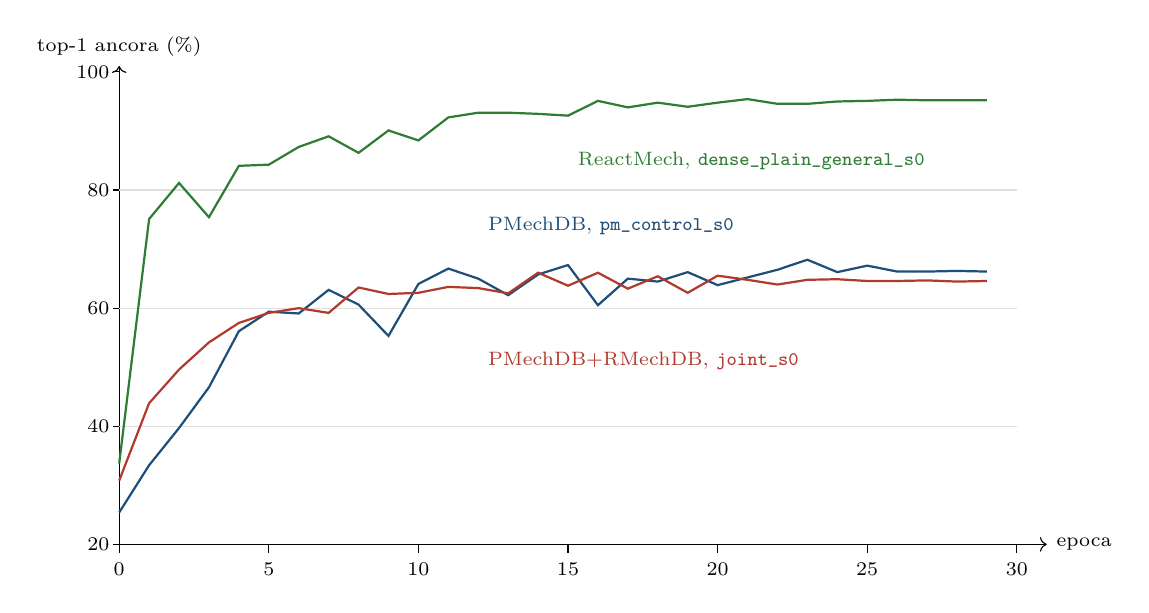
\begin{tikzpicture}[x=0.38cm,y=0.075cm]
  % assi top-1
  \draw[->] (0,20) -- (31,20) node[right,font=\scriptsize]{epoca};
  \draw[->] (0,20) -- (0,101) node[above,font=\scriptsize]{top-1 ancora (\%)};
  \foreach \y in {20,40,60,80,100} {\draw (-0.2,\y) -- (0,\y) node[left,font=\scriptsize]{\y};}
  \foreach \x in {0,5,10,15,20,25,30} {\draw (\x,20) -- (\x,18.5) node[below,font=\scriptsize]{\x};}
  \foreach \y in {40,60,80} {\draw[gray!25] (0,\y) -- (30,\y);}
  \draw[ksblu,thick] plot coordinates {(0,25.4) (1,33.4) (2,39.7) (3,46.6) (4,56.1) (5,59.4) (6,59.1) (7,63.1) (8,60.6) (9,55.3) (10,64.1) (11,66.7) (12,65.0) (13,62.2) (14,65.7) (15,67.3) (16,60.5) (17,65.0) (18,64.5) (19,66.1) (20,63.9) (21,65.2) (22,66.5) (23,68.2) (24,66.1) (25,67.2) (26,66.2) (27,66.2) (28,66.3) (29,66.2)};
  \draw[ksrosso,thick] plot coordinates {(0,30.8) (1,43.9) (2,49.6) (3,54.2) (4,57.5) (5,59.2) (6,60.0) (7,59.2) (8,63.5) (9,62.4) (10,62.6) (11,63.6) (12,63.4) (13,62.5) (14,66.0) (15,63.8) (16,66.0) (17,63.3) (18,65.4) (19,62.6) (20,65.5) (21,64.8) (22,64.0) (23,64.8) (24,64.9) (25,64.6) (26,64.6) (27,64.7) (28,64.5) (29,64.6)};
  \draw[ksverde,thick] plot coordinates {(0,33.7) (1,75.1) (2,81.2) (3,75.4) (4,84.1) (5,84.3) (6,87.3) (7,89.1) (8,86.3) (9,90.1) (10,88.4) (11,92.3) (12,93.1) (13,93.1) (14,92.9) (15,92.6) (16,95.1) (17,94.0) (18,94.8) (19,94.1) (20,94.8) (21,95.4) (22,94.6) (23,94.6) (24,95.0) (25,95.1) (26,95.3) (27,95.2) (28,95.2) (29,95.2)};
  \node[font=\scriptsize,ksverde,anchor=west] at (15,85) {ReactMech, \code{dense_plain_general_s0}};
  \node[font=\scriptsize,ksblu,anchor=west] at (12,74) {PMechDB, \code{pm_control_s0}};
  \node[font=\scriptsize,ksrosso,anchor=west] at (12,51) {PMechDB+RMechDB, \code{joint_s0}};
\end{tikzpicture}

\medskip
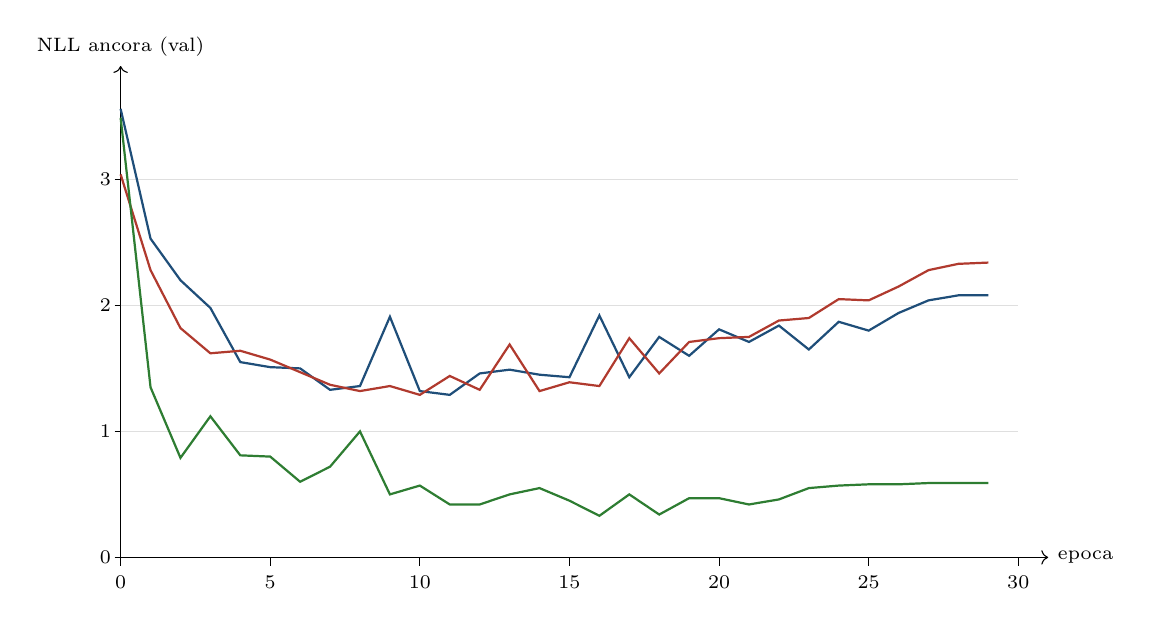
\begin{tikzpicture}[x=0.38cm,y=1.6cm]
  \draw[->] (0,0) -- (31,0) node[right,font=\scriptsize]{epoca};
  \draw[->] (0,0) -- (0,3.9) node[above,font=\scriptsize]{NLL ancora (val)};
  \foreach \y in {0,1,2,3} {\draw (-0.2,\y) -- (0,\y) node[left,font=\scriptsize]{\y};}
  \foreach \x in {0,5,10,15,20,25,30} {\draw (\x,0) -- (\x,-0.07) node[below,font=\scriptsize]{\x};}
  \foreach \y in {1,2,3} {\draw[gray!25] (0,\y) -- (30,\y);}
  \draw[ksblu,thick] plot coordinates {(0,3.56) (1,2.53) (2,2.20) (3,1.98) (4,1.55) (5,1.51) (6,1.50) (7,1.33) (8,1.36) (9,1.91) (10,1.32) (11,1.29) (12,1.46) (13,1.49) (14,1.45) (15,1.43) (16,1.92) (17,1.43) (18,1.75) (19,1.60) (20,1.81) (21,1.71) (22,1.84) (23,1.65) (24,1.87) (25,1.80) (26,1.94) (27,2.04) (28,2.08) (29,2.08)};
  \draw[ksrosso,thick] plot coordinates {(0,3.04) (1,2.28) (2,1.82) (3,1.62) (4,1.64) (5,1.57) (6,1.47) (7,1.37) (8,1.32) (9,1.36) (10,1.29) (11,1.44) (12,1.33) (13,1.69) (14,1.32) (15,1.39) (16,1.36) (17,1.74) (18,1.46) (19,1.71) (20,1.74) (21,1.75) (22,1.88) (23,1.90) (24,2.05) (25,2.04) (26,2.15) (27,2.28) (28,2.33) (29,2.34)};
  \draw[ksverde,thick] plot coordinates {(0,3.49) (1,1.35) (2,0.79) (3,1.12) (4,0.81) (5,0.80) (6,0.60) (7,0.72) (8,1.00) (9,0.50) (10,0.57) (11,0.42) (12,0.42) (13,0.50) (14,0.55) (15,0.45) (16,0.33) (17,0.50) (18,0.34) (19,0.47) (20,0.47) (21,0.42) (22,0.46) (23,0.55) (24,0.57) (25,0.58) (26,0.58) (27,0.59) (28,0.59) (29,0.59)};
\end{tikzpicture}
\caption{Validazione per epoca. Sopra: top-1 dell'ancora. Sotto: NLL dell'ancora. Blu:
\code{pm_control_s0}; rosso: \code{joint_s0} (validazione congiunta PMechDB \code{closed_base} + RC);
verde: ReactMech \code{dense_plain_general_s0}.}
\label{fig:curve}
\end{figure}

\scoperta{sovra-confidenza dopo l'epoca 10--14}{La loss di training scende fino a circa 0{,}05
(PMechDB) mentre la NLL dell'ancora in validazione tocca il minimo tra le epoche 8 e 14 (circa
1{,}3) e poi risale fino a 2{,}1--2{,}3 alla trentesima epoca, mentre il top-1 resta su un plateau
attorno al 65\%. Il modello continua a ordinare bene ma diventa sovra-confidente sugli errori. La
selezione di \code{best.pt} sul top-1 dell'ancora (non sulla NLL) protegge l'accuratezza, ma
probabilità calibrate (necessarie per la ricerca su reti di reazione) richiederanno early stopping
sulla NLL, regolarizzazione o calibrazione a posteriori.}

% ---------------------------------------------------------------------
\section{Importanza per permutazione degli input}
\label{sec:ris-importance}
\code{ksmech-eval importance} (9 novembre) permuta ciascuna colonna di input dei token (e blocchi di
colonne correlate) tra i token dello stesso tipo della parte valutata, e misura l'aumento della NLL
dell'ancora e la caduta di top-1/3 rispetto al baseline; le feature di coppia non sono toccate. Run
\code{pm_v19_s0}, PMechDB molecule val, 1\,241 campioni, baseline top-1 dell'ancora 65{,}8\%,
NLL 1{,}24, 3 ripetizioni.

\begin{table}[H]
\centering
\caption{Importanza per permutazione (\code{pm_v19_s0}): caduta di top-1 dell'ancora in punti
percentuali e aumento della NLL dell'ancora, ordinati per effetto.}
\label{tab:importance}
\begin{tabular}{@{}llrr@{}}
\toprule
Gruppo & Tipo & $\Delta$ top-1 (pt) & $\Delta$ NLL\\
\midrule
elemento ($Z$) & atomo, categorico & $-43{,}6$ & $+4{,}57$\\
carica formale & atomo, categorico & $-30{,}2$ & $+1{,}98$\\
blocco Fukui ($f^+$, $f^-$, duale) & atomo & $-18{,}3$ & $+0{,}79$\\
carica di Mulliken & atomo & $-13{,}9$ & $+0{,}71$\\
$V^{\mathrm{bur}}$ & atomo & $-5{,}3$ & $+0{,}37$\\
$f^-$ (orbitali congelati) & atomo & $-5{,}3$ & $+0{,}21$\\
$f^+$ (orbitali congelati) & atomo & $-5{,}1$ & $+0{,}16$\\
blocco pesi di frontiera (HOMO$-1$\dots LUMO$+1$) & atomo & $-4{,}3$ & $+0{,}19$\\
descrittore duale & atomo & $-3{,}9$ & $+0{,}12$\\
peso LUMO & atomo & $-2{,}6$ & $+0{,}10$\\
peso LUMO$+1$ & atomo & $-1{,}2$ & $+0{,}06$\\
peso HOMO$-1$ & atomo & $-0{,}9$ & $+0{,}04$\\
energia $E_r$ e frazione conservata & orbitale & $0{,}0$ & $+0{,}002$\\
insieme spettrale & orbitale & $-0{,}1$ & $-0{,}03$\\
ogni altro descrittore orbitale & orbitale & $|\Delta|<0{,}6$ & $|\Delta|<0{,}03$\\
segno di chiralità & atomo & $0{,}0$ & $0{,}0$\\
\bottomrule
\end{tabular}
\end{table}

\scoperta{gli input orbitali hanno poca importanza marginale}{Elemento e carica formale dominano,
seguiti dai descrittori di reattività per atomo (Fukui, Mulliken, $V^{\mathrm{bur}}$, pesi di
frontiera), che insieme valgono decine di punti. I descrittori propri dei token orbitali (pesi sui
centri, quote $s/p/d$, coseni, popolazione di sovrapposizione, insieme spettrale) valgono ciascuno meno
di mezzo punto. Due cautele: l'importanza per permutazione sottostima le feature ridondanti (un token
orbitale eredita gli embedding dei suoi atomi attraverso i pesi sui centri, quindi gran parte della sua
informazione è già presente), e la fisica orbitale entra soprattutto attraverso le feature di coppia
($G$, $g_2$), che questo esperimento non permuta. La misura dice quindi che, nella forma attuale, i
token orbitali agiscono soprattutto come supporto delle feature di coppia, non come portatori
autonomi di informazione.}

% ---------------------------------------------------------------------
\section{Ablazione dei token orbitali (10 novembre)}
\label{sec:ris-ablazione-orb}
L'importanza per permutazione non distingue un input ridondante da uno inutile: un modello riaddestrato
può spostare il lavoro su un altro input. Per questo l'ablazione è stata addestrata. Quattro bracci, 3 seed
ciascuno, split per molecola, preset general, encoder denso, senza augmentation di risonanza, 30 epoche,
selezione su \code{closed_base} val: (a) come \code{pm_v19_s0}; (b) senza le 25 colonne orbitali
(\code{--drop-token-features orbital}, occupazione inclusa); (c) come (b) e senza insieme spettrale; (d)
come (c) e senza embedding ereditati. Un solo pod vast.ai con una RTX 5090 (torch 2.14.1+cu130, codice
\code{79a402f}), 3 fit per GPU, circa 80 minuti ciascuno; il braccio (a) è stato riaddestrato lì perché
un riferimento deve girare sulla stessa GPU e la stessa torch dei suoi bracci (la lezione del passo 9 di
P9). Il riferimento coincide con quello locale: \code{orb_a_s0} 63{,}2/81{,}2/86{,}5 contro i
62{,}4/81{,}4/86{,}0 di \code{pm_v19_s0}. Decodifica con beam 5, caps legacy, \code{DECODE_VERSION} 5.

\begin{table}[H]
\centering
\caption{Ablazione orbitale, full-R top-1/3/5 per seed e media (\%). PMechDB \code{closed_base} val
($n=1\,238$) e ReactMech molecule val fuori distribuzione ($n=911$, i checkpoint PMechDB decodificati sui
campioni ReactMech). \enquote{any}: un esito registrato qualsiasi.}
\label{tab:ablazione-orb}
\small
\begin{tabular}{@{}lllrr@{}}
\toprule
Braccio & Set & seed 0 / 1 / 2 (top-1/3/5) & media top-1 / 3 & top-1 any\\
\midrule
a & PMechDB & 63{,}2/81{,}2/86{,}5; 65{,}8/82{,}3/86{,}3; 66{,}2/85{,}1/87{,}9 & 65{,}05 / 82{,}88 & 67{,}56\\
b & PMechDB & 66{,}6/85{,}6/89{,}5; 63{,}4/84{,}9/88{,}2; 61{,}5/84{,}1/86{,}6 & 63{,}81 / 84{,}87 & 66{,}48\\
c & PMechDB & 63{,}7/80{,}5/86{,}1; 63{,}0/80{,}5/86{,}0; 66{,}5/81{,}9/84{,}2 & 64{,}38 / 80{,}96 & 67{,}29\\
d & PMechDB & 63{,}9/83{,}2/86{,}8; 65{,}2/84{,}0/88{,}8; 67{,}4/85{,}5/87{,}9 & 65{,}48 / 84{,}22 & 68{,}09\\
\midrule
a & ReactMech & 54{,}1/71{,}0/73{,}7; 52{,}3/72{,}8/75{,}7; 49{,}6/69{,}6/72{,}0 & 51{,}99 / 71{,}13 & 53{,}71\\
b & ReactMech & 49{,}2/71{,}2/74{,}0; 51{,}4/69{,}8/72{,}4; 52{,}6/69{,}0/73{,}4 & 51{,}04 / 70{,}03 & 52{,}58\\
c & ReactMech & 56{,}5/73{,}8/76{,}9; 46{,}7/69{,}2/73{,}1; 49{,}2/67{,}4/70{,}8 & 50{,}79 / 70{,}11 & 51{,}99\\
d & ReactMech & 54{,}8/71{,}7/74{,}3; 48{,}7/70{,}3/73{,}8; 53{,}6/69{,}0/71{,}4 & 52{,}36 / 70{,}33 & 53{,}82\\
\bottomrule
\end{tabular}
\end{table}

\begin{table}[H]
\centering
\caption{Confronti appaiati con il braccio (a) (\code{ksmech-eval compare}): differenza delle medie in
punti, tra parentesi il $p$ di McNemar unilaterale \enquote{il braccio è peggiore} quando è sotto 0{,}25.
Nessun braccio supera la tolleranza della regola U20.}
\label{tab:ablazione-orb-cmp}
\small
\begin{tabular}{@{}llrrrrl@{}}
\toprule
Set & Braccio & top-1 own & top-1 any & top-3 own & top-3 any & tolleranza\\
\midrule
PMechDB & b & $-1{,}24$ (0{,}11) & $-1{,}08$ (0{,}17) & $+1{,}99$ & $+1{,}67$ & 3{,}0--4{,}3\\
PMechDB & c & $-0{,}67$ & $-0{,}27$ & $-1{,}91$ (0{,}053) & $-1{,}83$ (0{,}036) & 2{,}9--3{,}4\\
PMechDB & d & $+0{,}43$ & $+0{,}54$ & $+1{,}35$ & $+1{,}32$ & 3{,}3--3{,}4\\
\midrule
ReactMech & b & $-0{,}95$ (0{,}050) & $-1{,}13$ (0{,}054) & $-1{,}10$ (0{,}13) & $-1{,}61$ (0{,}030) & 2{,}5--4{,}0\\
ReactMech & c & $-1{,}21$ (0{,}063) & $-1{,}72$ (0{,}040) & $-1{,}02$ (0{,}013) & $-1{,}61$ (0{,}003) & 5{,}2--8{,}2\\
ReactMech & d & $+0{,}37$ & $+0{,}11$ & $-0{,}80$ (0{,}24) & $-1{,}10$ (0{,}22) & 2{,}7--5{,}5\\
\bottomrule
\end{tabular}
\end{table}

\paragraph{Importanza a blocchi dei tre \code{orb_a}.} Su PMechDB il blocco Fukui costa 19--22 punti di
top-1 e i pesi di frontiera 4--7; ogni blocco orbitale sposta il top-1 al più di 1{,}6 punti e la NLL tra
$-0{,}12$ e $+0{,}05$. Su ReactMech il blocco Fukui costa 13--17 punti, e le quote $s/p/d$, le quote $p$, le
quote $d$ e i pesi sui centri alzano la NLL in tutti i 12 casi blocco-seed (top-1 fino a $-2{,}0$); i
blocchi energia, coppia di centri e quota $s$ restano a circa 0. Sui cinque casi da manuale il seed
sposta i ranghi quanto il braccio, e nessun braccio trova l'addizione 1,4 del cianuro all'acroleina.

\scoperta{le colonne orbitali servono fuori distribuzione}{Alla lettera della regola nessun braccio
fallisce, quindi le colonne sarebbero ridondanti. Ma la regola non vede un effetto sotto circa 3 punti
(deviazione standard tra seed 1{,}4--2{,}1, per (c) fino a 4 su ReactMech), e due misure indipendenti
concordano fuori distribuzione: i bracci senza colonne perdono 1--1{,}7 punti su ReactMech, e il modello
completo legge proprio i blocchi di forma (quote $s/p/d$, pesi sui centri) su ReactMech mentre li ignora
su PMechDB. Le colonne portano un piccolo pezzo di ciò che si trasferisce a molecole nuove, come il token
orbitale della specifica intende. \textbf{Decisione dell'utente (10 novembre)}: il token orbitale tiene
le sue 25 colonne per ora; quali togliere si decide più avanti.}

\scoperta{i pesi di frontiera si trasferiscono male}{Su ReactMech permutare i pesi di frontiera degli
atomi \emph{alza} il top-1 in due seed su tre ($+5{,}5$ e $+3{,}8$ punti), mentre su PMechDB costa 4--7
punti: il modello impara da quei pesi una regola che vale nel dominio di training e non fuori.}

% ---------------------------------------------------------------------
\section{Il modello all'indietro (10 novembre)}
\label{sec:ris-backward}
\code{bwd_s0}--\code{bwd_s2}: sullo stesso pod e con lo stesso codice, \code{--direction backward} con
le opzioni del braccio (a). Lo store all'indietro è stato costruito in locale (un pod non ha i record QM,
e ogni file di token verifica il suo record: costruito sul pod lo store aveva 0 campioni); i token del
lato prodotto non presenti nello store 19 (3\,565) sono stati spediti prima dei fit.

\begin{table}[H]
\centering
\caption{Modello all'indietro su \code{closed_base} val dei campioni all'indietro ($n=1\,233$), full-R
(\%). \enquote{any}: un qualsiasi pool padre registrato.}
\label{tab:backward}
\begin{tabular}{@{}lrrrrr@{}}
\toprule
Run & top-1 & top-3 & top-5 & top-1 any & top-3 any\\
\midrule
\code{bwd_s0} & 61{,}4 & 78{,}8 & 82{,}3 & 63{,}0 & 80{,}8\\
\code{bwd_s1} & 57{,}8 & 74{,}9 & 80{,}0 & 59{,}9 & 78{,}2\\
\code{bwd_s2} & 59{,}0 & 77{,}9 & 80{,}9 & 61{,}2 & 80{,}3\\
\midrule
media & 59{,}4 & 77{,}2 & 81{,}1 & 61{,}4 & 79{,}8\\
\bottomrule
\end{tabular}
\end{table}

Il passo precedente è predetto quasi bene quanto il successivo: il braccio (a) in avanti fa 63{,}2--66{,}2
al top-1 sulla propria \code{closed_base} val, il modello all'indietro 57{,}8--61{,}4, con la stessa
architettura e gli stessi input. La migliore epoca per l'ancora è la 24 (\code{bwd_s0}, top-1
dell'ancora 63{,}2\%) contro la 26 di \code{orb_a_s0} (65{,}3\%). Il modello all'indietro è l'espansore
della retrosintesi e il secondo termine del riordinatore per andata e ritorno (sezione~\ref{sec:roundtrip}),
la cui valutazione è il passo successivo.
% =====================================================================
\chapter{Scoperte e lezioni}
\label{ch:scoperte}
% =====================================================================
Questo capitolo raccoglie, in ordine tematico, le scoperte principali fatte durante lo sviluppo; i
capitoli precedenti ne danno il contesto e i numeri.

\section{Sulla fisica}
\begin{enumerate}
\item \textbf{La geometria di contatto peggiora il ranking.} Ogni tentativo di valutare l'accoppiamento
  di Klopman--Salem a una geometria di contatto (tabella di van der Waals, MLP, kernel orientato
  analitico, lobi sul sito) ha classificato la prima freccia peggio del solo fattore di gap $G$ (test
  top-1: testa congelata $\sim$3\%, $\mathrm{KS}_3+\mathrm{KS}_2$ 14{,}3\%, $G$ 20{,}4\%). La tabella di
  contatto favorisce sistematicamente gli H e gli shell $s$; il lobo di un orbitale di legame punta al
  partner. L'avvicinamento non è una proprietà dei reagenti: è stato tolto dal modello (spec v9).
\item \textbf{$G$ va calcolato sugli spettri canonici completi.} Le energie diagonali degli LMO non
  rispettano neppure l'ordine $\sigma^*$(C--Cl) $>$ $\sigma^*$(C--Br) $>$ $\sigma^*$(C--I); i pesi
  spettrali sì. Troncare lo spettro a 8 voci cambia $G$ fino al 21{,}8\%.
\item \textbf{La fisica da sola porta l'ancora al primo posto una volta su sei} (floor 15{,}6\% su
  PMechDB), contro circa 65\% del modello addestrato; il ranker GBDT sulle sole feature geometry-free
  arriva al 48\% sulla prima freccia. La fisica è un segnale reale ma non sufficiente.
\item \textbf{$g_2$ conta sui radicali}: sul floor dei passi radicalici il gap a due livelli migliora il
  top-1 (13{,}5\% contro 11{,}7\%) e nella suite radicalica sposta i ranghi attesi, ma nelle ablazioni
  addestrate né $G$ né $g_2$ da soli sono peggiori dell'altro.
\item \textbf{Gli input orbitali hanno poca importanza marginale.} L'importanza per permutazione mostra
  che il modello si appoggia a elemento, carica formale e descrittori di reattività per atomo; ogni
  descrittore orbitale vale meno di mezzo punto. Ipotesi: ridondanza con le feature di coppia e con gli
  embedding ereditati dagli atomi; da verificare con un'ablazione (capitolo~\ref{ch:futuro}).
\end{enumerate}

\section{Sui dati e sulle etichette}
\begin{enumerate}[resume]
\item \textbf{Le frecce non sono un bersaglio ben posto.} Un orbitale localizzato non distingue il
  doppietto dal legame ionico (Mitsunobu, O--Li); dopo molte regole il round trip si fermava al
  99{,}67\%. Prevedere $\vb R$ ha risolto il problema alla radice (copertura dal 92\% al 99{,}6\%).
\item \textbf{Il plateau del 60\% era in parte simmetria}: nel 21{,}5\% della validazione l'etichetta
  sceglie uno di più atomi equivalenti, e i pareggi in bf16 contavano come hit. La chiusura per
  simmetria ha portato \code{flex_first} da 55{,}9\% a 63{,}9\% senza riaddestrarlo.
\item \textbf{RDKit non è un oracolo di risonanza}: la chiave enumerata concorda tra le forme di un
  prodotto solo nel 59\% dei casi; RDKit raggiunge il prodotto disegnato in 147 delle 471 coppie di
  risonanza; restituisce forme con H rigenerati e radicali spuri. La chiave sigma (senza enumerazione) è
  esatta.
\item \textbf{Il rumore delle etichette ReactMech valeva 6 punti}: ridisegnare il prodotto nella
  struttura di Kekulé più vicina al reagente ha portato la validazione ReactMech da 85\% a 91\% senza
  riaddestrare.
\item \textbf{Le regole di cancellazione toglievano proprio i segnali utili}: la regola \enquote{tipo
  $d$} rimuoveva più di metà del peso sull'ancora annotata nel 15{,}2\% dei passi; renderle canali ha
  dato una configurazione (GENERAL) non peggiore.
\item \textbf{Gli esclusi non erano radicali}: nessuno dei 290 passi esclusi da PMechDB e dal pilota
  ReactMech era un passo radicalico; quasi tutti erano errori di disegno (metili senza H, catalizzatori
  senza leganti, fosfine di Pd(0) disegnate come fosfonio su un metallo neutro).
\item \textbf{Lo split per molecola deve guardare anche i prodotti}: con i soli reagenti il 32\% dei
  collegamenti tra passi attraversava le parti; i reagenti comuni legano il 78\% dei passi in un gruppo,
  quindi validazione e test sono fuori distribuzione per costruzione.
\item \textbf{Il test ReactMech per molecola è sbilanciato} su famiglie mai viste (Swern, cromo):
  top-1 da $\sim$91\% a $\sim$72\%.
\item \textbf{Il punto di sella lineare dei carbeni}: ETKDG disegna CCl$_2$ lineare; da lì il
  tripletto sembra più basso; da una partenza spostata il singoletto vince di 1\,eV. Da qui le leggi delle
  due partenze e di \code{BOND_FORMED}.
\end{enumerate}

\section{Sul training e sulla valutazione}
\begin{enumerate}[resume]
\item \textbf{GENERAL non costa accuratezza}: leggere tutte le celle con i flag e gli extra orbitali dà
  65{,}6\% contro 64{,}5\% (entro il rumore): le esclusioni a mano non servono al modello.
\item \textbf{Le sorgenti si trasferiscono in modo asimmetrico}: PMechDB$\to$ReactMech 52\%,
  ReactMech$\to$PMechDB 28\%. ReactMech è facile ma stretto.
\item \textbf{L'addestramento congiunto con i radicali costa circa 2 punti sui passi polari}
  (\code{joint} 63{,}1\% contro \code{pm_control} 65{,}2\%, McNemar $p=0{,}085$, 5 coppie di seed su 9
  significative), mentre i passi polari aiutano i radicalici (69{,}7\% congiunto contro 63{,}1\% solo
  RMechDB).
\item \textbf{Sovra-confidenza}: la NLL di validazione tocca il minimo tra le epoche 8 e 14 e poi
  risale, mentre il top-1 resta su un plateau; il modello non ha dropout. La selezione per top-1
  protegge l'accuratezza ma non la calibrazione.
\item \textbf{Il confondimento hardware}: nove ablazioni addestrate su RTX 5090/cu130 confrontate con
  un riferimento su RTX 3090/cu126 si spostano tutte nella stessa direzione; non sono interpretabili
  finché il riferimento non è rieseguito sulla stessa macchina.
\item \textbf{Il determinismo dipende dai thread}: gli alberi di LightGBM cambiano con il numero di
  thread (deterministico solo a numero di thread fisso); il beam decoder cambia un campione su un
  quasi-pareggio tra 3 e 4 thread di torch.
\item \textbf{NaN può sembrare perfezione}: una run fp16 diventata NaN segnava top-1 1{,}000 e aveva
  sovrascritto \code{best.pt}; da qui le regole di arresto sui valori non finiti.
\item \textbf{Due metriche diverse}: il top-1 full-R della decodifica supera il top-1 dell'ancora del
  training perché valuta l'intera classe e cinque ancore.
\item \textbf{I token orbitali contano fuori distribuzione, non dentro}: tolte le 25 colonne orbitali
  nessun braccio peggiora su PMechDB, ma su ReactMech si perdono 1--1{,}7 punti (McNemar
  $p=0{,}003$--$0{,}06$) e il modello completo legge lì le quote $s/p/d$ e i pesi sui centri. La regola di
  tolleranza non vede effetti sotto circa 3 punti: per un input fisico serve anche un set fuori
  distribuzione.
\item \textbf{Il passo precedente è imparabile quasi quanto il successivo}: stesso modello, 59\% contro
  65\% al top-1 full-R.
\item \textbf{Un riferimento va rieseguito sulla macchina dei bracci}: rifatto sulla 5090, il braccio (a)
  dell'ablazione orbitale coincide con il riferimento locale (63{,}2 contro 62{,}4), e i confronti
  diventano leggibili.
\end{enumerate}

\section{Sulla rete di reazione e sulla termochimica}
\begin{enumerate}[resume]
\item \textbf{Una chiave che azzera le cariche unisce prodotti diversi}: le due eterolisi di un legame
  avevano la stessa chiave di pool nel decoder, che ne teneva una sola; lo ha rivelato il modello
  all'indietro, per cui ogni inversa di un'addizione catione--anione è un'eterolisi.
\item \textbf{Un fallimento di featurizzazione non è chimica}: un pool senza token prendeva l'88\% della
  massa come vicolo cieco; ora è \code{EXPAND_FAILED} e la sua massa conta come incertezza.
\item \textbf{L'ordine dei frammenti cambia la previsione}: lo stesso pool scritto in due ordini dà
  $\log P$ diverse di 3{,}5 unità; la rete ordina i frammenti per chiave, il training no.
\item \textbf{Alcuni record QM sono selle}: ottimi L-BFGS-B partiti da geometrie simmetriche restano su
  torsioni metiliche immaginarie; seguire il modo abbassa $G$ fino a 1{,}8\,kcal/mol e toglie i salti della
  regola di xtb.
\item \textbf{ALPB dipende dall'orientazione}: 0{,}02--0{,}15\,kcal/mol su $G-E_{\mathrm{el}}$, irrilevante
  rispetto all'errore di GFN2 ma visibile nei test.
\item \textbf{Il benchmark umano condivide il disegno di PMechDB, non i suoi passi}: 326 specie in comune
  per chiave, ma solo 11 pathway su 350 con ogni passo nel training.
\item \textbf{RDKit perde l'E/Z dei doppi legami d'anello} quando toglie idrogeni espliciti: la correzione
  alla radice non ha spostato nessuna chiave su 126\,068 frammenti.
\end{enumerate}

\section{Sull'ingegneria}
\begin{enumerate}[resume]
\item \textbf{Provenienza come vincolo, non come documentazione}: ogni artefatto porta i suoi input, i
  loader rifiutano gli obsoleti, training e valutazione rifiutano gli alberi sporchi; una modifica di un
  file tracciato durante una build ne invalida gli output.
\item \textbf{Instabilità hardware}: i riavvii sotto carico erano BIOS e RAM, non il software; un
  worker senza limite ai thread BLAS bastava però a saturare la macchina.
\item \textbf{La CPU e il QM}: l'ottimizzazione domina il tempo; OpenBLAS nei worker (1{,}5--2{,}7$\times$)
  e l'ottimizzatore ANC/RFO ($3{,}1\times$) sono pronti, il secondo non ancora di default perché
  richiederebbe il ricalcolo completo della cache.
\end{enumerate}
% =====================================================================
\chapter{Applicazione web ChemRho, client e server MCP}
\label{ch:serve}
% =====================================================================
L'app web (\code{ksmech.serve}) è un componente aggiuntivo: il motore non la importa mai (lo verifica
\code{tests/test_engine_boundary.py}) e le sue dipendenze sono un gruppo separato (FastAPI 0.142.2,
uvicorn 0.54.0, SQLModel, pydantic 2.13.5, markdown-it-py). Il marchio dell'interfaccia è
\textbf{ChemRho}; il codice resta \code{ksmech}.

\section{Struttura a strati}
113 moduli e 26\,101 righe in 17 sotto-pacchetti, in un monolite modulare a un processo. Le
fondamenta sono una catena, \code{core} $\to$ \code{compute} $\to$ \code{chem} $\to$ \code{science}
$\to$ \code{predict} $\to$ \code{runtime}, dove ogni strato importa solo quelli precedenti;
\code{depiction} poggia su \code{core}; i pacchetti funzionali (\code{pool}, \code{workbench},
\code{embedding}, \code{browse}, \code{curate}, \code{ml}, \code{accounts}, \code{ocr}, \code{content})
importano le fondamenta ma mai l'uno l'altro; \code{app} collega tutto. Un test analizza gli import con
l'AST e verifica che il grafo consentito sia aciclico. Una route è sottile: controlla gli id, chiama una
funzione di servizio e ne restituisce il valore.

\begin{table}[H]
\centering
\caption{Sotto-pacchetti dell'app web (righe).}
\label{tab:serve}
\small
\begin{tabular}{@{}lrp{10.6cm}@{}}
\toprule
Pacchetto & Righe & Contenuto\\
\midrule
\code{core} & 4\,187 & impostazioni, errori, DB di curation, chiavi, versioni e fingerprint, capability e profili, autenticazione, audit, schemi (1\,693 righe, rispecchiati in TypeScript)\\
\code{chem} & 3\,353 & normalizzazione, featurizzazione (tre modi), pool, geometrie dei metalli (860), base STO-$n$G, cubi, Hückel esteso sintetico\\
\code{predict} & 3\,353 & predittori, rete di reazione (849), espansione, job (730)\\
\code{depiction} & 2\,244 & depiction 2D lato server con RDKit, template prospettici\\
\code{workbench} & 1\,852 & molecola, insiemi orbitali, densità, proprietà, simmetria\\
\code{browse} & 1\,460 & indice e ricerca di PMechDB e dei passi curati\\
\code{app} & 1\,345 & cablaggio FastAPI, CLI\\
\code{science} & 1\,305 & $G^{\mathrm{atom}}$, lettura delle frecce, analisi, applicazione dei passi\\
\code{accounts} & 1\,251 & utenti, sessioni, password, OIDC, quote\\
\code{curate} & 1\,223 & curation, ricontrollo, esportazione\\
\code{ocr} & 1\,145 & motore OCR (MolScribe), installazione\\
altri & 3\,378 & \code{compute} (worker), \code{runtime}, \code{pool}, \code{ml}, \code{embedding}, \code{content} (wiki)\\
\bottomrule
\end{tabular}
\end{table}

\section{Calcolo, chimica e predittori}
\paragraph{Worker di calcolo.} Uno scheduler a processi (\code{ProcessScheduler}) con 1--2 worker
\emph{spawned}, coda a priorità (interattivo $<$ job $<$ background) con deduplicazione per chiave,
deadline con SIGKILL (\code{WORKER_TIMEOUT}), interruttore dopo più di 5 timeout o crash in 600\,s
(\code{WORKER_UNSTABLE}, 503), riciclo del worker dopo 500 task o 2\,048\,MB. Una richiesta interattiva
attende al più 15\,s e poi restituisce 202 \emph{Pending}.

\paragraph{Modi della chimica.} \code{real}: cache condivise in sola lettura, poi \code{data/serve}; una
mancanza esegue GFN2-xTB nel worker. \code{cached}: solo cache (\code{FEATURIZATION_DISABLED}).
\code{synthetic}: Hückel esteso iterato sulla carica nella base di valenza GFN2 (veicolo di test,
\enquote{mai un'affermazione chimica}). I metalli di transizione usano geometrie iniziali con template di
coordinazione (metodo \code{+metal-geom-v1}): su 33 complessi, da 19 corretti a 27 corretti.

\paragraph{Predittori.} \code{floor} (ancore per $|G^{\mathrm{atom}}|$, completate dai canali dominanti;
punteggio in 1/eV, non una probabilità), \code{gbdt} (il ranker LightGBM sulle coppie di orbitali),
\code{network} (un checkpoint locale di \code{ksmech-train} con il decoder del motore, su CPU; punteggi
$\log P(\vb R)$; la testa di stop non è letta), \code{user} (pseudo-predittore per le correzioni).
L'espansione applica ogni candidato come $\vb B+\vb R$ e raggruppa i prodotti per chiave di pool; la
rete di reazione (\code{ksmech-serve/network-v2}) ha nodi per id di pool, archi per (stato, $\vb R$),
cammini ordinati per peso, motivi terminali (\code{NO_CANDIDATES}, \code{TURNOVER}, \code{MAX_STEPS},
\code{NODE_BUDGET}); parametri di default: beam 5, 8 passi, 200 nodi.

\paragraph{Predict e Correct sulle matrici di reazione.} Il contratto (\code{docs/serve_v9_contract.md})
scambia $\vb R$ come \texttt{\{bonds: [i,j,delta], lone: [i,delta]\}}, l'ancora, la lettura in frecce
(decomposizione in mosse di coppie come \emph{perfect matching} che massimizza il $|G|$ diretto) e la
lettura orbitale (coppia di token, $G$, coppia canonica dominante con le energie). Correct è un editor di
$\vb R$ (strumenti legame, doppietto, freccia, gomma).

\section{Funzioni dell'interfaccia}
Frontend React 19 + TypeScript 6 + Vite 8, RDKit.js e 3Dmol (184 file, 21\,488 righe; pacchetto di
visualizzazione \code{@ksmech/viz} di 90 file e 12\,723 righe, solo props, formato di scena JSON
versionato). Quattro sezioni:
\begin{description}[style=nextline]
\item[ChemPtah (\texttt{\#/workbench})] sketcher 2D con scorciatoie in stile ChemDraw, lunghezze e
  angoli fissi, template, CIP; esportazione SVG/PNG/PDF/LaTeX (chemfig) con stile ACS; importazione da
  immagine via OCR; vista 3D con superfici orbitali (valutazione separabile della base GTO: da 2{,}8--3{,}9\,s
  a 0{,}02\,s per orbitale), diagramma dei livelli, proprietà, gruppo puntuale.
\item[ClotoMech (\texttt{\#/predict}, \texttt{\#/correct}, \texttt{\#/curate})] previsione di reti con viste
  Scheme e Pathways e viste del passo (Textbook, Animated, Orbitals); correzione; curation dei meccanismi
  (stati predicted, validated, corrected, rejected; esportazione come record PMechDB grezzi, mai dati di
  training).
\item[ChemThot (\texttt{\#/browse})] ricerca esatta (sotto-multiinsieme di chiavi di specie) e per
  sottostruttura su PMechDB e sui passi curati.
\item[Wiki (\texttt{\#/wiki})] pagine Markdown con front matter TOML renderizzate dal server
  (\code{index}, \code{reaction-matrix}, \code{orbital-tokens}, \code{klopman-salem},
  \code{sn2-example}) e \code{llms.txt}.
\end{description}
Altre funzioni: traccia degli embedding di un pool attraverso un checkpoint (job \enquote{trace});
account con password locali (scrypt) o OIDC (ORCID, Google), sessioni in cookie HttpOnly, ruoli reader
$<$ user $<$ curator $<$ admin, quote (user 100 al giorno e 10 al minuto); profili \code{lab} e
\code{public} (il profilo pubblico disabilita browse, curate, export, embedding e ml: i dati di PMechDB
non devono mai essere raggiungibili online, e un test percorre ogni route dell'app pubblica); log di audit
di ogni richiesta che modifica; OCR con MolScribe 1.1.1 in un ambiente isolato (\code{tools/ocr}, torch
CPU 2.5.1, timeout 60\,s). Test end-to-end: Playwright con il Chrome di sistema, 10 file di specifiche, 30
test.

\section{Client HTTP e server MCP}
\code{ksmech} è una CLI sopra \code{KsmechClient} (header \code{X-Ksmech-Via: cli}; comandi
\code{health}, \code{meta}, \code{predict}, \code{jobs}, \code{check}, \code{pool}, \code{molecule},
\code{depict2d}, \code{ocr}, \code{ml}, \code{embedding}, \code{curate}, \code{browse}; exit 0/1/2).
\code{ksmech-mcp} (FastMCP, \code{mcp==1.30.0}) espone 20 strumenti sopra lo stesso client, registrati in
base alle capability di \code{/api/meta}; tutti in sola lettura tranne \code{predict_mechanism}. L'API
HTTP è l'unico contratto.
% =====================================================================
\chapter{Lavoro futuro e questioni aperte}
\label{ch:futuro}
% =====================================================================

\section{Questioni aperte immediate}
\begin{itemize}
\item \textbf{Rieseguire \code{joint} sulla RTX 5090} (\code{ONLY=joint_r}, circa 2 ore) per decidere i
  nove bracci addestrati del passo 9 di P9.
\item Il braccio con la maschera dei metalli $d$ (iv) e i flag delle soglie (xi: $\tau_{\mathrm{atom}}$,
  fusione spettrale), che richiedono ricostruzioni dello store o dei token.
\item Il costo di circa 2 punti dell'addestramento congiunto; \code{pm_v19} a un solo seed.
\item Le parti di test di \code{closed_base} (per le configurazioni open-shell) e di RC non ancora lette.
\item Casi di dominio lasciati all'utente: l'addotto Et$_3$B--O$_2$ (\code{SPIN_NOT_CONSERVED}), la legge
  per i singoletti che collassano (non carbeni), le esclusioni di ozono e persolfato, il costo
  dell'etichetta di \code{reactmech-7172766faa0ff062}, l'estensione dello snapshot ReactMech per molecola
  (224 ritorni di P5 sono \code{SPLIT_CONFLICT}), uno split ReactMech per classi.
\item Calibrazione: early stopping o regolarizzazione sulla NLL (sovra-confidenza dopo l'epoca
  10--14); il modello non ha dropout.
\item Infrastruttura: caricare i checkpoint dei passi 8 e 9 sul dataset privato, pubblicare \code{main}
  (deciso dall'utente il 10 novembre, solo codice, dopo il controllo \code{tests/test_p8_no_flower_lines.py}),
  decidere se passare a \code{tblite-anc} come ottimizzatore di default (ricalcolo completo del QM),
  regola dei plateau anche per i gusci chiusi, un arbitro DFT per gli stati di spin.
\item Differiti dal piano open-shell: D1 (il CSV ufficiale di RMechDB), D2 (spGFN2 per $u>0$, ablazione
  dopo P9), D3 (catene radicaliche USPTO di FlowER e una testa \code{END_MECH} addestrata: oggi nessuna
  sorgente produce \code{stop_label}); le fasi
  dell'app web S1--S3.
\item Pre-addestramento dell'encoder su QMugs: dati in preparazione, obiettivo non ancora definito dalla
  specifica.
\end{itemize}

\section[Quali colonne orbitali togliere]{Quali colonne orbitali togliere (\texttt{docs/todo.md})}
L'ablazione (sezione~\ref{sec:ris-ablazione-orb}) ha tenuto le 25 colonne. I blocchi energia, coppia di
centri e quota $s$ non mostrano uso su nessuno dei due set; le quote $s/p/d$ e i pesi sui centri servono
su ReactMech. Prossimo passo: un braccio con solo le colonne scelte tolte (\code{--drop-token-features
NOME...}), 3 seed, giudicato su ReactMech val oltre che su \code{closed_base} val, con la regola di
tolleranza e con McNemar.

\section{La rete di reazione: ciò che resta}
Il codice di ogni elemento del piano (A--L) è in \code{main} con test e voci del registro; resta calcolo,
dati e calibrazione:
\begin{itemize}
\item la termochimica delle specie che una rete raggiunge (\code{ksmech-qm thermo}, su richiesta);
\item QM e token per i 17\,595 passi di catena ReactMech fuori dal pilota, perché i benchmark della
  sezione 5 del piano possano girare (le specie del benchmark umano sono fatte: 1\,056 su 1\,072);
\item la valutazione del riordinatore per andata e ritorno: QM delle specie figlie del beam, griglia di
  $\lambda$ su entrambi i set di val; poi la ricerca bidirezionale (I1);
\item la calibrazione dei parametri (\code{step_cost}, $\varepsilon$ e margine, budget di salita,
  tolleranza di massa: nessuna reazione registrata deve essere un falso pozzo) e le misure del
  \enquote{fatto quando} del piano, tra cui i nodi espansi dal grafo delle specie contro quello dei pool;
\item questioni lasciate aperte: se un turnover resta assorbente una volta che le energie libere esistono;
  se una classe all'indietro debba ammettere anche i membri in avanti negati (l'unione); il costo esatto
  dei passi con due prodotti usati (iper-flusso intero); un atom mapper per i bersagli non mappati; un
  valore appreso alla Retro*, proof-number search o MCTS; l'invarianza del modello all'ordine dei
  frammenti come augmentation di training; i lettori a valle per un solvente diverso dall'acqua; se
  ingerire le catene ReactMech in \code{steps.parquet} (cambierebbe lo split).
\end{itemize}

\paragraph{Note di ricerca.} Una rassegna dell'utente (\code{reports/Deep learning ricerca
combinatoria.md}, 8 novembre) su deep learning e ottimizzazione combinatoria conclude che, per \ksm, il
floor non addestrato del fattore di gap è il controllo che il modello appreso deve battere \emph{dentro
la stessa ricerca} a parità di calcolo, che una ricerca best-first alla Levin è un'alternativa garantita
al beam, e che conviene un training consapevole della ricerca (LaSO, DAgger).
% =====================================================================
\appendix
\chapter{Codici di motivo}
\label{app:codici}
% =====================================================================
Ogni passo o molecola esclusi sono contati sotto un codice. Elenco dei principali.

\begin{longtable}{@{}p{6.2cm}p{9.6cm}@{}}
\caption{Codici di motivo per livello.}\label{tab:codici}\\
\toprule
Codice & Significato\\
\midrule
\endfirsthead
\toprule Codice & Significato\\ \midrule
\endhead
\multicolumn{2}{@{}l}{\emph{Ingest e validazione}}\\
\code{SANITIZE_FAILED} & valenze non valide per RDKit (complessi ate ipervalenti)\\
\code{UNBALANCED}, \code{MAP_NOT_BIJECTIVE} & atomi pesanti non bilanciati; mappe non biiettive\\
\code{BOND_NOT_FOUND}, \code{ARROWS_MISMATCH} & legame sorgente assente; le frecce non riproducono i prodotti\\
\code{RADICAL_ARROW} & freccia a un elettrone in una sorgente polare (0 casi)\\
\code{DUPLICATE_STEP} & riga FlowER con la stessa reazione canonica (553)\\
\midrule
\multicolumn{2}{@{}l}{\emph{Dominio}}\\
\code{RESONANCE_STEP} & interconversione di risonanza (diventa coppia di risonanza)\\
\code{NULL_STEP}, \code{NONCONJUGATED_SHIFT} & lati identici; stessa chiave senza flusso bilanciato\\
\code{METAL_PLACEHOLDER} & metallo disegnato senza leganti\\
\code{CHARGE_UNREPAIRED} & errore di carica che nessuna legge ripara\\
\code{RADICAL_DRAWN} & atomo radicalico in un passo polare fuori dalle leggi dei gusci aperti\\
\code{MULTIPLICITY_UNTABULATED}, \code{_AMBIGUOUS} & nessun conteggio di spin dalle tabelle\\
\code{SPIN_NOT_CONSERVED} & $u$ non conservato dal passo\\
\code{NOT_ELEMENTARY} & voce atomica dispari in un passo polare, o classe non elementare\\
\code{SOMO_NOT_INTEGRAL} & SOMO non intera (smearing) in un frammento a guscio aperto\\
\code{MULTI_RADICAL_SPECIES} & specie non metallica con $u\ge2$ che non è un caso di Hund\\
\code{SPIN_CENSUS_REFUSED} & specie che il censimento di spin tiene fuori dal QM\\
\code{SET_STEP}, \code{DISSOCIATIVE_ET_STEP} & trasferimento di singolo elettrone; trasferimento dissociativo\\
\code{SPLIT_CONFLICT} & passo nuovo che unisce gruppi congelati in parti diverse\\
\code{LEAK_GUARD} & passo rmechdb con una specie della validazione/test PMechDB (run congiunte)\\
\midrule
\multicolumn{2}{@{}l}{\emph{Classi di dominio (ammesse, contate)}}\\
\code{REPAIRED_DATIVE}, \code{_V1}, \code{_A1}, \code{_BL} & riparazioni conservate\\
\code{METAL_SUSPECT} & metallo 3d lasciato d$^1$--d$^9$ in un frammento pari (flag)\\
\code{PAIRED_DRAWING}, \code{HIGH_SPIN_DRAWING} & ridisegni di spin\\
\code{RADICAL_SPECTATOR}, \code{RADICAL_REACTIVE} & passi polari con un radicale ammesso\\
\code{CARBENE_SINGLET}, \code{OSM_CU2}, \code{OSM_FE3} & carbeni di singoletto; Cu(II) e Fe(III) a guscio aperto\\
\midrule
\multicolumn{2}{@{}l}{\emph{QM}}\\
\code{OPT_NOT_CONVERGED}, \code{SCF_NOT_CONVERGED} & limiti di iterazione (500/250, retry 2\,000/1\,000)\\
\code{TIMEOUT}, \code{EMBED_FAILED} & oltre 900\,s (retry 3\,600); embedding impossibile\\
\code{CONNECTIVITY_CHANGED}, \code{RESTRAINED_GEOM} & legame rotto oltre $1{,}3\times$; geometria con vincoli (avviso)\\
\code{SPIN_PARITY}, \code{BOND_FORMED} & numero di elettroni incompatibile; l'ottimo forma un legame\\
\code{WORKER_CRASH}, \code{FUKUI_SCF_FAIL} & crash del worker; SCF a $N\pm1$ fallito (avviso)\\
\midrule
\multicolumn{2}{@{}l}{\emph{Campioni, training, decodifica}}\\
\code{MISSING_TOKENS}, \code{NO_BOND_INDEX} & token o indici di Wiberg mancanti\\
\code{STALE_ARTIFACT} & artefatto obsoleto o da albero sporco\\
\code{TOO_LARGE} & più di 1\,024 token\\
\code{DROPPED_DOMAIN_CLASS} & classe tolta per ablazione\\
\code{NONFINITE} & run fermata per valori non finiti (exit 3)\\
\code{DECODE_DROPPED:*} & \code{CHARGE_NOT_CONSERVED}, \code{OCTET_EXCEEDED}, \code{FORMAL_CHARGE_RANGE},
  \code{ODD_OFF_BROKEN_BOND}, \code{CLOSED_MINUS1}, \code{RESONANCE_ONLY_STEP}\dots\\
\code{DECODE_MERGED}, \code{DECODE_ANCHOR_UNCOMPLETED} & completazione già trovata; ancora senza completazione\\
\code{OWN_KEY_MISMATCH}, \code{SIBLING_KEY_FAILED} & hit proprio con chiave diversa; passo illeggibile per i fratelli\\
\code{CHILD_INVALID} & figlio illeggibile da RDKit nel riordinamento per andata e ritorno\\
\midrule
\multicolumn{2}{@{}l}{\emph{Termochimica}}\\
\code{IMAGINARY_INVERTED}, \code{_DROPPED} & regola di xtb sui modi immaginari residui (avvisi)\\
\code{IMAGINARY_REOPTIMIZED}, \code{_PERSISTENT} & ri-ottimizzazione riuscita; modo rimasto\\
\code{REOPT_ROUNDS}, \code{REOPT_NO_LOWER_MINIMUM}, \code{REOPT_BUDGET} & motivi di stop della ri-ottimizzazione\\
\code{HESSIAN_ASYMMETRIC}, \code{SYMMETRY_FAILED} & $|H-H^T|>10^{-2}$; gruppo puntuale non trovato ($\sigma=1$)\\
\code{UNKNOWN_METHOD}, \code{RECORD_KEY_MISMATCH} & metodo senza solvente; SMILES del record diverso dalla chiave\\
\midrule
\multicolumn{2}{@{}l}{\emph{Rete di reazione}}\\
\code{DEPTH_CUT}, \code{CYCLE}, \code{EXPANSION_BUDGET}, \code{POP_BUDGET} & tagli della ricerca\\
\code{MAPPING_FAILED} & bersaglio non mappato sull'inizio: ricerca a costo uniforme\\
\code{SINK_AT_T}, \code{TURNOVER}, \code{NO_OUTGOING_STEP}, \code{EXPAND_FAILED} & stati assorbenti\\
\code{UNEXPLORED}, \code{CLIMB_CUT}, \code{EQUILIBRIUM} & massa inesplorata; oltre il budget di salita; classe senza assorbimento\\
\code{ONE_WAY}, \code{REVERSE_MISSING}, \code{NO_FREE_ENERGY} & arco senza inverso; inverso non valutabile; pool senza $G$\\
\code{NO_NET_REACTION}, \code{START_IS_GOAL} & nessuna reazione netta; bersaglio già nel pool iniziale\\
\code{SELF_LOOP}, \code{PARTNER_ONLY}, \code{MASS_DIVERGED} & grafo delle specie: scambio degenere; passo dei soli partner; massa infinita\\
\code{NOT_USING_BYPRODUCT} & retrosintesi: passo che non tocca il sottoprodotto\\
\bottomrule
\end{longtable}

% =====================================================================
\chapter{Versioni}
\label{app:versioni}
% =====================================================================
\begin{table}[H]
\centering
\caption{Costanti di versione nel codice attuale.}
\label{tab:versioni}
\small
\begin{tabular}{@{}p{4.4cm}p{3.6cm}p{7.6cm}@{}}
\toprule
Costante & Valore & Storia\\
\midrule
specifica & v10.1 & v3 $\to$ v7.2 (IBO) $\to$ v8 ($\vb R$) $\to$ v8.1 (chiave sigma) $\to$ v9 (niente stage B) $\to$ v9.1/9.2 $\to$ v10 $\to$ v10.1 (rete di reazione)\\
\code{SAMPLE_VERSION} & 19 & tabella~\ref{tab:sampleversion}\\
token \code{SCHEMA_VERSION} & 10 & 7$\to$8 (degeneri), 9 (IBO), 10 (extra, P0a)\\
record QM \code{SCHEMA_VERSION} & 1 & invariato\\
\code{FLOOR_VERSION} & 4 & 2 (P0), 3 (celle), 4 (\code{own_break})\\
\code{DECODE_VERSION} & 5 & 2 (P0), 3 (caps), 4 (schermo), 5 (\code{rank_any}, chiave di pool)\\
\code{FROZEN_SPLIT_SCHEMA} & 1 & \\
indice QM \code{INDEX_VERSION} & 3 & 2 dal P4 (spin), 3 (sidecar termici)\\
\code{THERMO_VERSION} & 1 & la ri-ottimizzazione aggiunge chiavi alla configurazione, non cambia la versione\\
\code{network_predict} & 1 & formato JSON di \code{ksmech-network predict --out}\\
\code{SPIN_RULE_VERSION} & \code{spin-rule-v2} & \\
tabelle di spin & \code{spin_table_v2}, \code{spin_theory_v2}, \code{metal_v1} & \\
\code{OPEN_SHELL_RULE} & \code{occ-plateau-v1} & P2b\\
\code{LGBM_VERSION}, \code{TRAIN_VERSION}, \code{IMPORTANCE_VERSION} & 1, 1, 1 & \\
\bottomrule
\end{tabular}
\end{table}

% =====================================================================
\chapter{Comandi tipici}
\label{app:comandi}
% =====================================================================
\begin{verbatim}
uv sync                                   # ambiente (torch ROCm)
uv sync --no-group rocm --group cuda      # host NVIDIA; poi export UV_NO_SYNC=1
uv run pytest -n 14 -m "not realdata"     # test di unita'
uv run pytest -m realdata                 # test su dati reali

uv run ksmech-data ingest --source pmechdb
uv run ksmech-qm run --source pmechdb --workers 8
uv run ksmech-qm bond-index
uv run ksmech-orbitals build --source pmechdb --workers 4
uv run ksmech-arrows samples --source pmechdb --workers 8
uv run ksmech-physics gbdt --source pmechdb --split molecule
uv run ksmech-eval floor --source pmechdb --split molecule

HSA_OVERRIDE_GFX_VERSION=10.3.0 uv run ksmech-train fit --run NOME \
    --preset general --no-resonance-draws --seed 0
uv run ksmech-train fit --run joint_s0 --preset open_shell \
    --source pmechdb+rmechdb --split pmechdb=molecule,rmechdb=rc_molecule \
    --val-cohort pmechdb=closed_base --no-resonance-draws

uv run ksmech-eval decode --run NOME --part val --beam 5 --cohort closed_base
uv run ksmech-eval compare --a A_s*/decode_hits_*.json --b B_s*/decode_hits_*.json
uv run ksmech-eval importance --run NOME --part val
uv run ksmech-serve --port 8000

uv run ksmech-arrows samples --source pmechdb --direction backward --workers 8
uv run ksmech-train fit --run bwd_s0 --direction backward --preset general
uv run ksmech-eval roundtrip --run orb_a_s0 --backward-run bwd_s0
uv run ksmech-qm run --species-from \
    data/processed/human_benchmark/qm_species.json
uv run ksmech-qm thermo --reopt-threshold -10 --reopt-rounds 3
uv run ksmech-network search --run NOME \
    --start 'CC(C)=O.C[O-]' --target 'CC(C)(O)OC'
uv run ksmech-network predict --run NOME \
    --start 'CC(C)=O.C[O-]' --free-energy qm
uv run ksmech-network retro-eval --run bwd_s0 --set human_benchmark
\end{verbatim}

% =====================================================================
\chapter{Glossario}
\label{app:glossario}
% =====================================================================
\begin{description}[style=nextline]
\item[Ancora] la voce di $\vb R$ attorno a cui è fattorizzata la previsione: un legame che si forma
  ($+1$) o, se nessuno, uno che si rompe ($-1$).
\item[Classe parsimoniosa] l'insieme delle matrici di reazione equivalenti (modulo risonanza e
  simmetria) con meno cariche formali e meno voci: l'etichetta di un passo.
\item[\code{closed_base}] la coorte di riferimento a guscio chiuso (PMechDB, split per molecola).
\item[Coppia di risonanza] un passo che interconverte due disegni della stessa specie, escluso dal
  bersaglio e conservato come esempio di equivalenza.
\item[Chiave di pool] le chiavi d'identità v2 dei frammenti di un pool, ordinate e unite da
  \enquote{.}: l'identità con cui decoder, rete e app web uniscono i pool.
\item[EXACT / SKELETON] i due livelli di arrivo della ricerca: le specie del bersaglio, oppure i loro
  scheletri pesanti con gli ordini di legame (a meno di protoni).
\item[Floor fisico] l'ordinamento delle ancore per $|G^{\mathrm{atom}}|$ senza parametri appresi.
\item[full-R top-$k$] frazione di campioni per cui una delle prime $k$ completazioni del beam è una
  variante della classe di etichette.
\item[Iper-cammino] un insieme di passi del grafo delle specie che produce il bersaglio da specie
  iniziali; un meccanismo a meno dell'ordine dei passi indipendenti.
\item[GENERAL / LEGACY] preset del modello: tutte le celle con flag ed extra orbitali, oppure gli
  input della v17.
\item[Modello all'indietro] lo stesso modello addestrato a predire $-\vb R$ dal pool figlio: il passo
  precedente.
\item[Lacuna (hole)] il gemello virtuale di un token a guscio aperto, che fa da accettore.
\item[Pool] il multiinsieme di tutte le specie presenti, scritto come una matrice $\vb B$.
\item[Release A / B] gli insiemi di fasi P1--P5 e P6--P8 (+P9) del piano open-shell.
\item[U20] la regola di tolleranza dei confronti appaiati.
\end{description}

\end{document}
